\ifdefined\isdraft
   \documentclass[25pt, landscape, draft]{foils}
\else
   \documentclass[25pt, landscape, final]{foils}
\fi

\usepackage{geometry}
\usepackage{graphicx}
\usepackage[usenames,dvipsnames,svgnames]{xcolor}
\usepackage{amsmath,amssymb,amsfonts} % Typical maths resource packages
\usepackage{multirow}
\usepackage[colorlinks=false,bookmarks=false,pageanchor=true]{hyperref}
\usepackage{authblk}
\usepackage{pstricks}
\usepackage{pst-node}

% Requires \documentclass{foils} in the preamble
\newcommand{\myfoilhead}[2]{\foilhead[#1]{\textcolor{blueDark}{\boldmath #2}}}

% Basic commonly used commands
\renewcommand\labelitemi{\textcolor{redDark}{$\bullet$}}
\renewcommand\labelitemii{\textcolor{greenDark}{$\bullet$}}
\renewcommand\labelitemiii{\textcolor{blueDark}{$\bullet$}}

\newcommand\arabicitemii{\textcolor{greenDark}{\textbf{\arabic{listcounter}.}}}

% Requires color package
% \usepackage{color}

\definecolor{redDark}{rgb}{0.8,0,0}
\definecolor{blueDark}{rgb}{0,0,0.5}
\definecolor{blueLight}{rgb}{0.5, 0.4, 1.0}
\definecolor{blue1}{rgb}{0.8, 0.8, 1.0}
\definecolor{greenDark}{rgb}{0, .5, 0}
\definecolor{greenDark2}{rgb}{0, .4, 0}
\definecolor{greenLight}{rgb}{.8, 1.0, .8}
\definecolor{yellowDark}{rgb}{.6, .6, 0}
\definecolor{black}{rgb}{0, 0, 0}
\definecolor{yellow}{rgb}{1.0, 1.0, 0.0}
\definecolor{bgColor}{rgb}{1,1,1}
\definecolor{pink}{rgb}{1.0,0.9,0.9}
\definecolor{greyLight}{rgb}{0.8,0.8,0.8}
\definecolor{greyDark}{rgb}{0.4,0.4,0.4}


\AtBeginDocument{\color{blueDark}}

% Common paper sizes: A4 210x297, Letter 279.4x215.9
\geometry{a4paper, landscape, includeall=true,
          centering=true, nomarginpar, headsep=0mm, headheight=0mm,
          tmargin=1mm, bmargin=1mm, lmargin=1mm, rmargin=1mm}

\hypersetup {
   pdfauthor={Dmitri Smirnov <d.s@plexoos.com>}
}


\MyLogo{}
\leftheader{}
\rightheader{\footnotesize \thepage/\pageref*{slide:last}}
\rightfooter{ 
\includegraphics[height=1.5\unitlength]{graphics/logo_doe} 
\includegraphics[height=1.5\unitlength]{graphics/logo_star} }
\Restriction{\footnotesize CHEP 2016 -- Dmitri Smirnov}

\setlength{\unitlength}{0.02\textwidth}
\psset{unit=\unitlength}
\psset{framearc=.1,fillcolor=blueDark!10,linecolor=blueDark,linewidth=0.1,fillstyle=solid,arrowscale=3}


\title{\vspace{20mm} \Huge Vertex Reconstruction at STAR\\[10mm]
\parbox{\textwidth}{\centering \small aka ``Primary Vertex finding in the RHIC high precision measurement era\\
enhancement and experience in STAR''}
}

\author{\quad\\[3mm]
Dmitri~Smirnov\\[3mm]
J.~Lauret, V.~Perevoztchikov, G.~Van~Buren, J.~Webb}

\affil{Brookhaven National Laboratory}

\date{\small October 13, 2016}


%===============================================================================
\begin{document}

\maketitle
\addtocounter{page}{1}

\small


%===============================================================================
\myfoilhead{-30mm}{Tracking with STAR Detector at RHIC}
%{{{

\noindent
\begin{pspicture}(0,0)(\textwidth,\textheight)


\rput[lt](0.03\textwidth,0.95\textheight){ 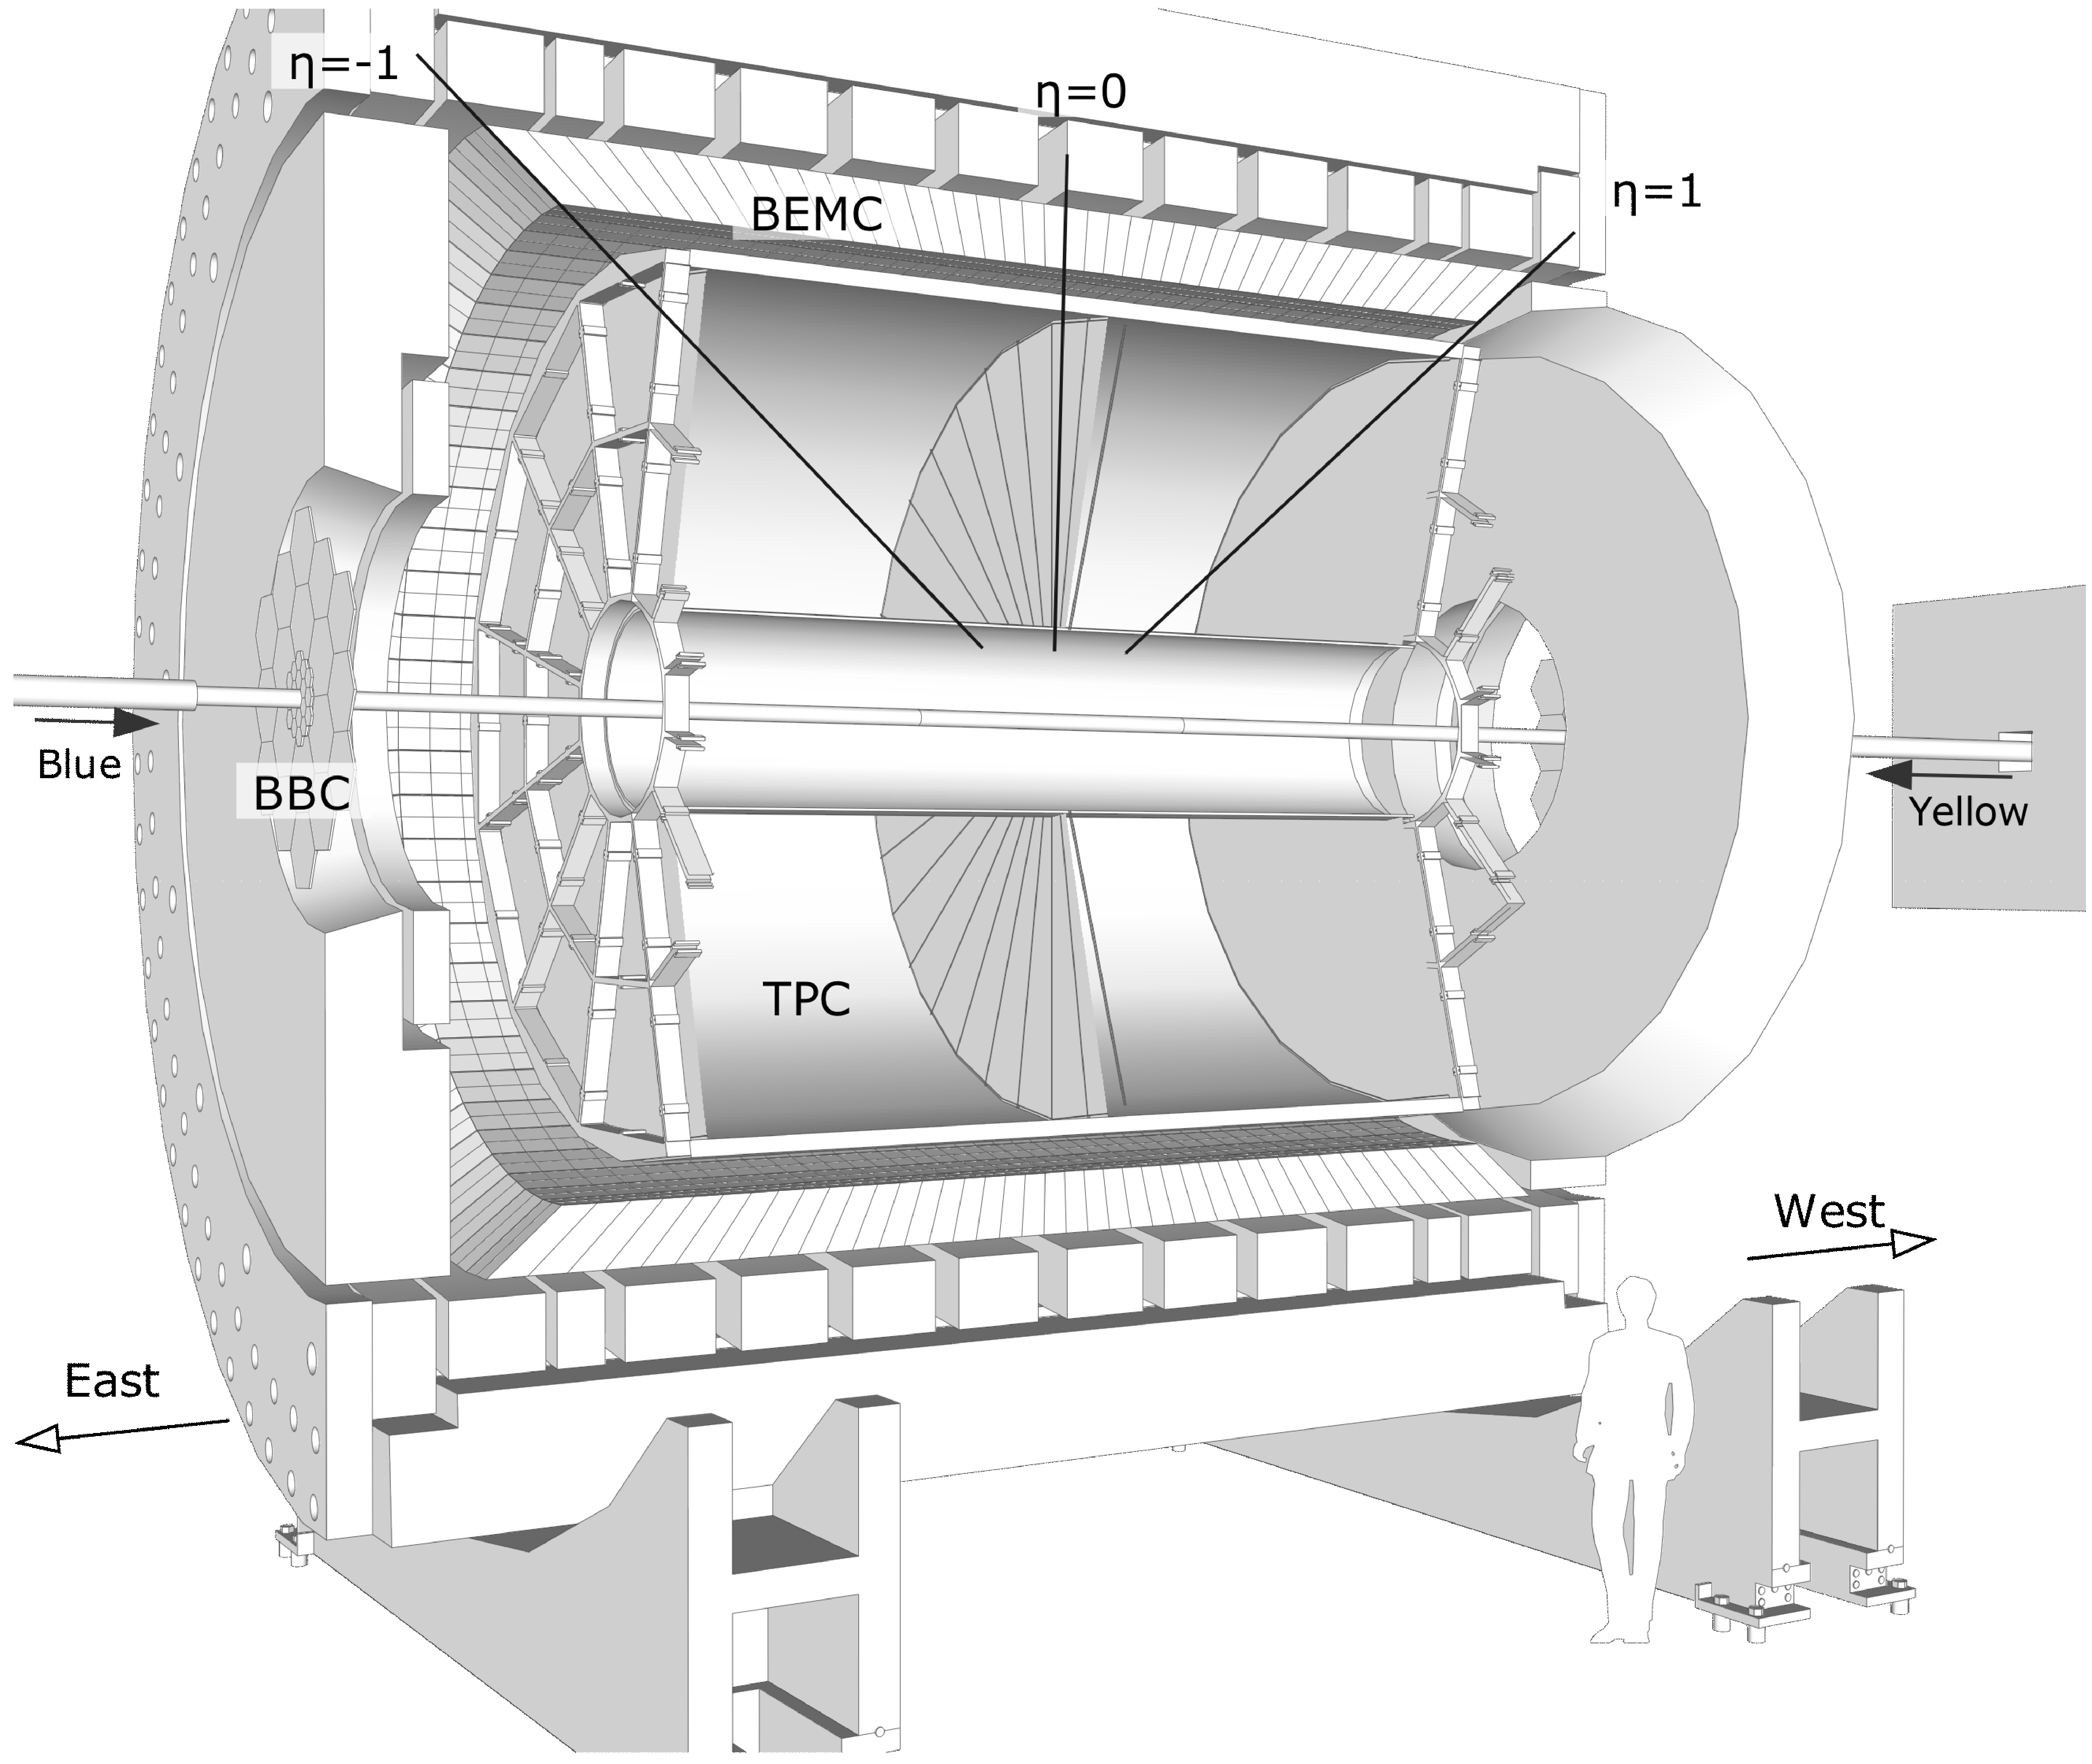
\includegraphics[height=0.5\textheight]{graphics/star_sectioncut_02} }
\rput[lt](0.48\textwidth,0.45\textheight){ 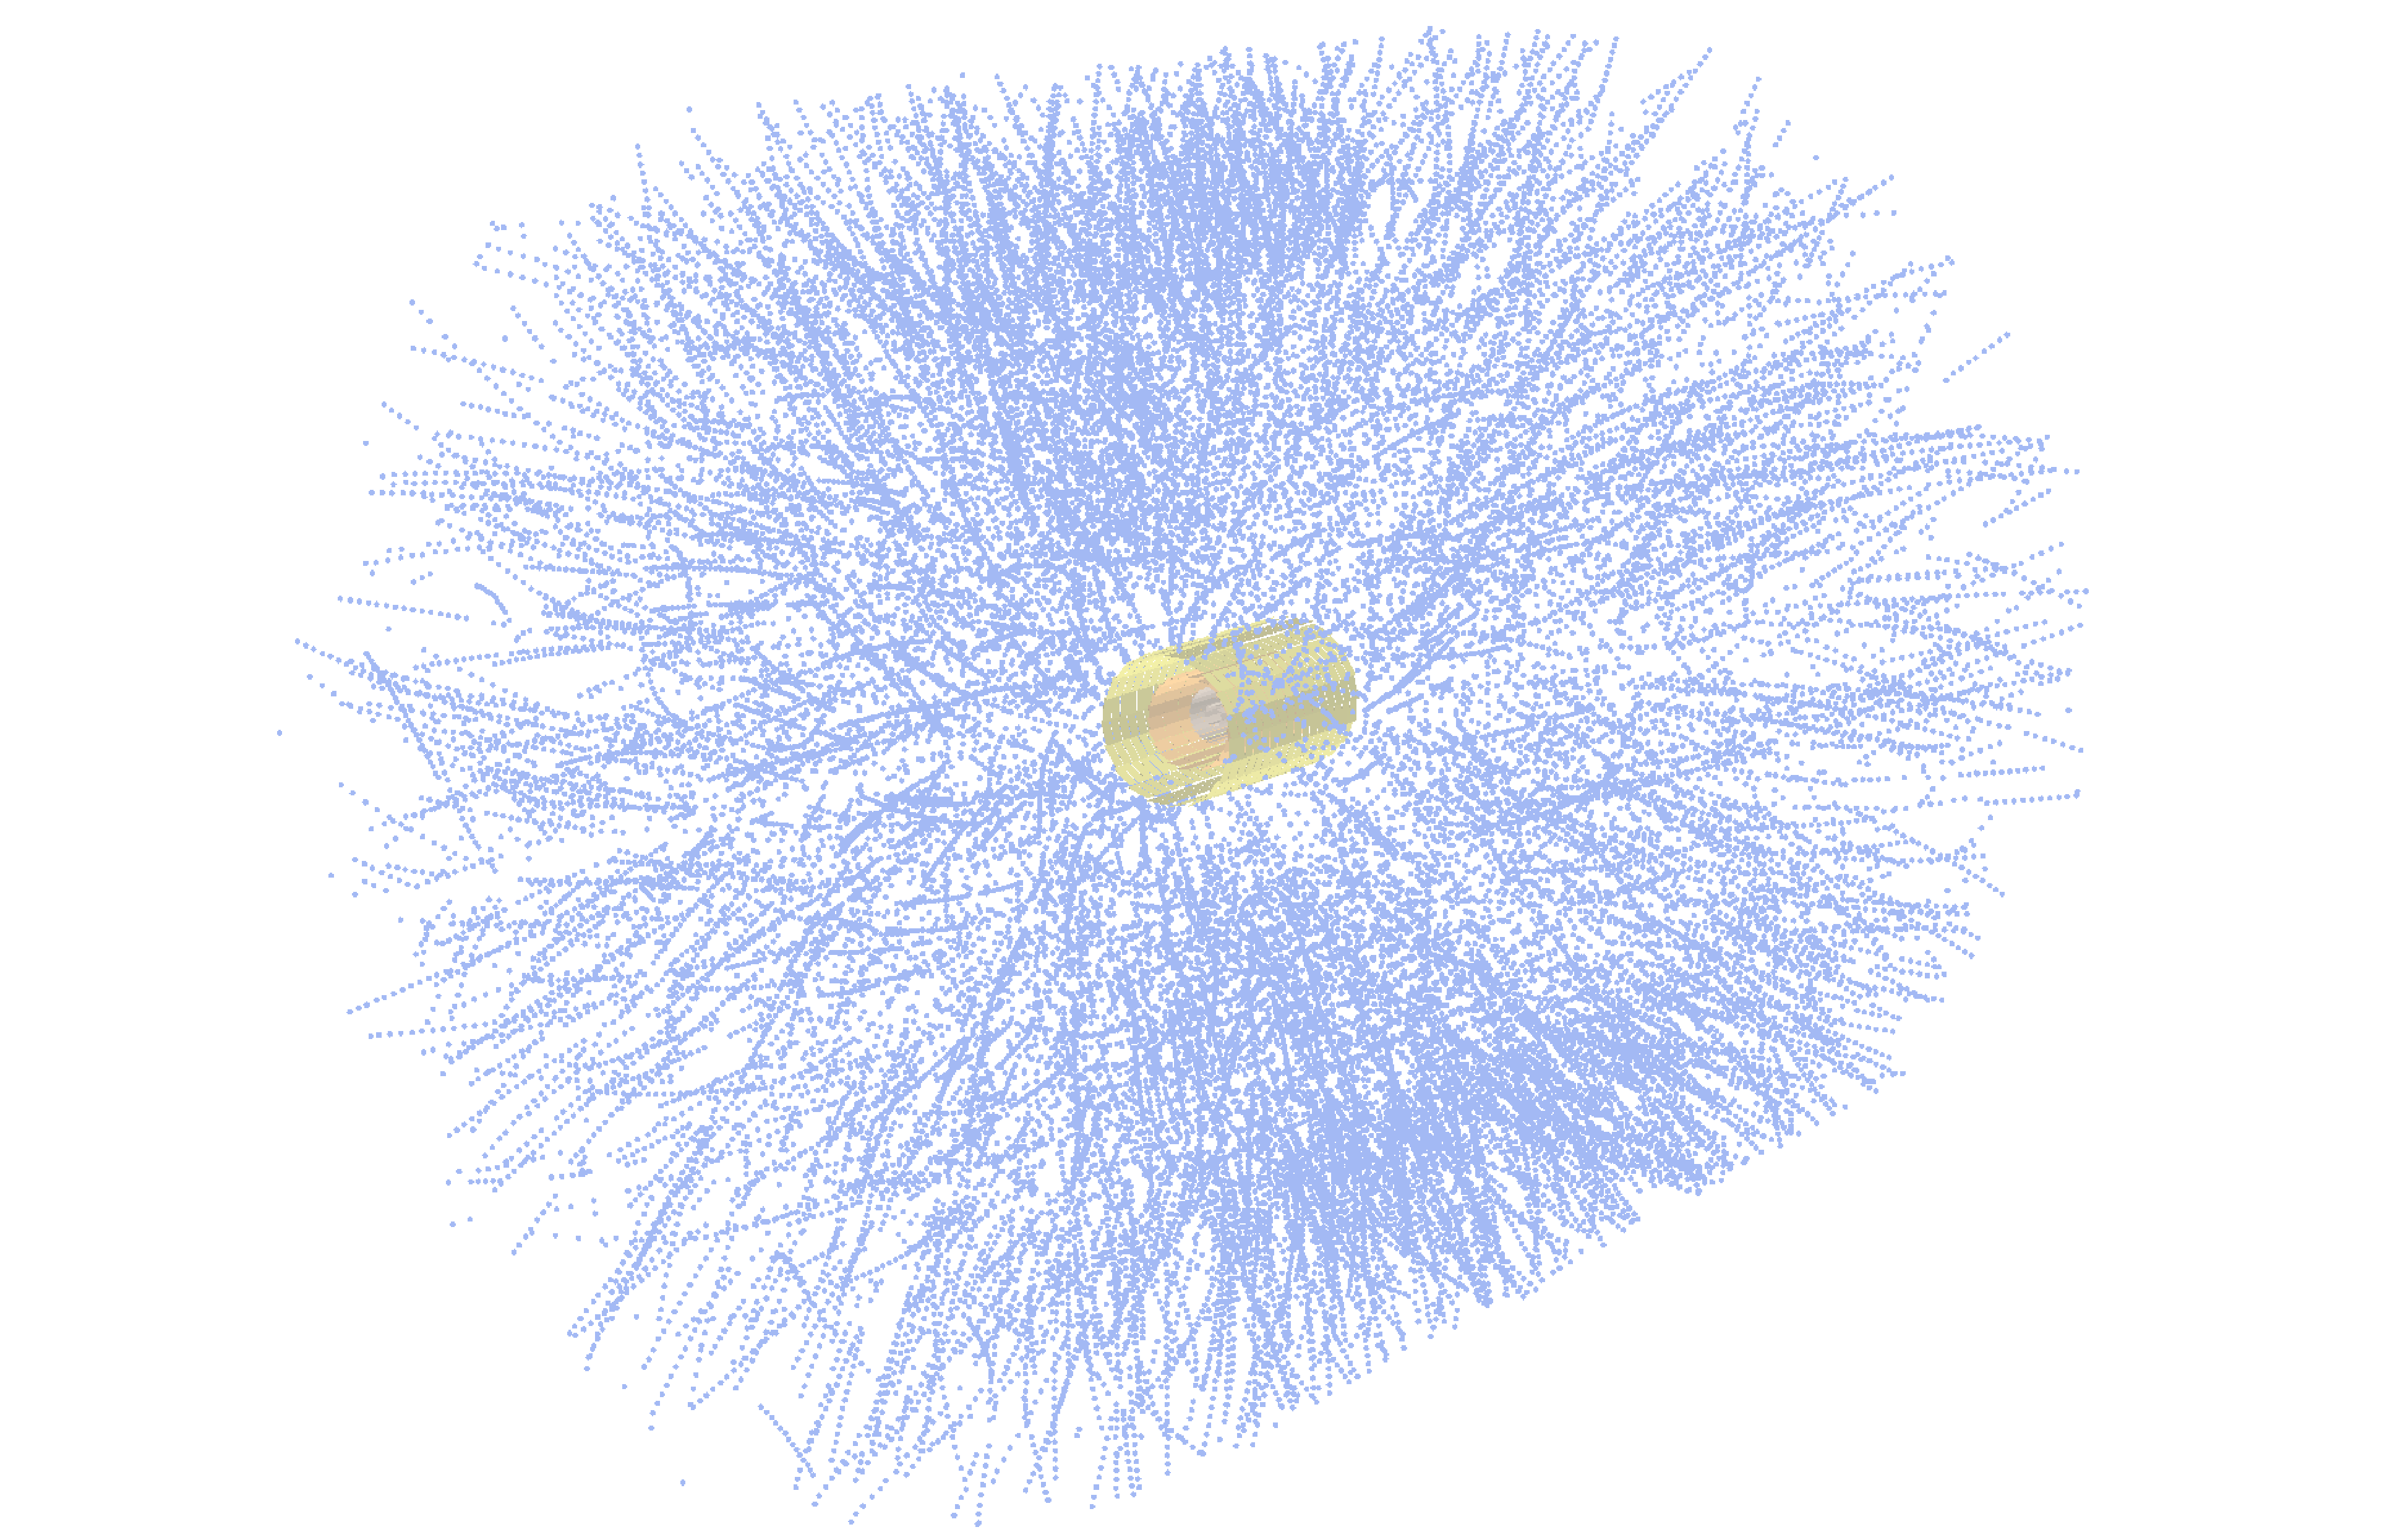
\includegraphics[height=0.5\textheight]{graphics/hijing_hits_light2} }


\rput[l](0.45\textwidth,0.70\textheight) {%
\begin{minipage}{0.55\textwidth}

\raggedright

\begin{list}{\labelitemi}{\setlength{\itemsep}{-2mm}
                          \setlength{\topsep}{0mm}}

   \item \textbf{STAR} is a versatile collider detector capable of detecting products of hadronic interactions

   \item \textbf{RHIC} provides polarized $\mathbf{pp}$ and unpolarized \textbf{heavy ion} (Au-Au, d-Au, Cu-Au, U-U, \dots) beams with $\sqrt{s}_{NN}$ up to 510~GeV

   \item \textbf{Rich physics program:} quark-gluon plasma, spin asymmetries, strange and
   charm particle decays

   \item Tracking at STAR is done by means of \textbf{Time Projection Chamber} (TPC)

\end{list}

\end{minipage}
}


\rput[rt](0.5\textwidth,0.37\textheight) {%
\begin{minipage}{0.45\textwidth}

\raggedright

\begin{list}{\labelitemi}{\setlength{\itemsep}{0mm}
                          \setlength{\topsep}{0mm}}

   \item STAR tracking delivered quality results for over a decade

   \begin{list}{\labelitemii}{\setlength{\itemsep}{0mm}
                              \setlength{\topsep}{-2mm}}

      \item STAR tracking is a robust deterministic algorithm consisting of seed finding stage followed by KF-based fitting

   \end{list}


   \item For STAR tracking details see talk by Jason~Webb (contribution \#286)

\end{list}

\end{minipage}
}


%\psgrid[gridlabels=0.7,subgriddiv=0, griddots=3](1,-1)(0,-3)(\textwidth,\textheight)

\end{pspicture}
%}}}



%===============================================================================
\myfoilhead{-30mm}{Precision Tracking with Heavy Flavor Tracker}
%{{{

\noindent
\begin{pspicture}(0,0)(\textwidth,\textheight)

\rput[rb](0.5\textwidth,0.35\textheight){ 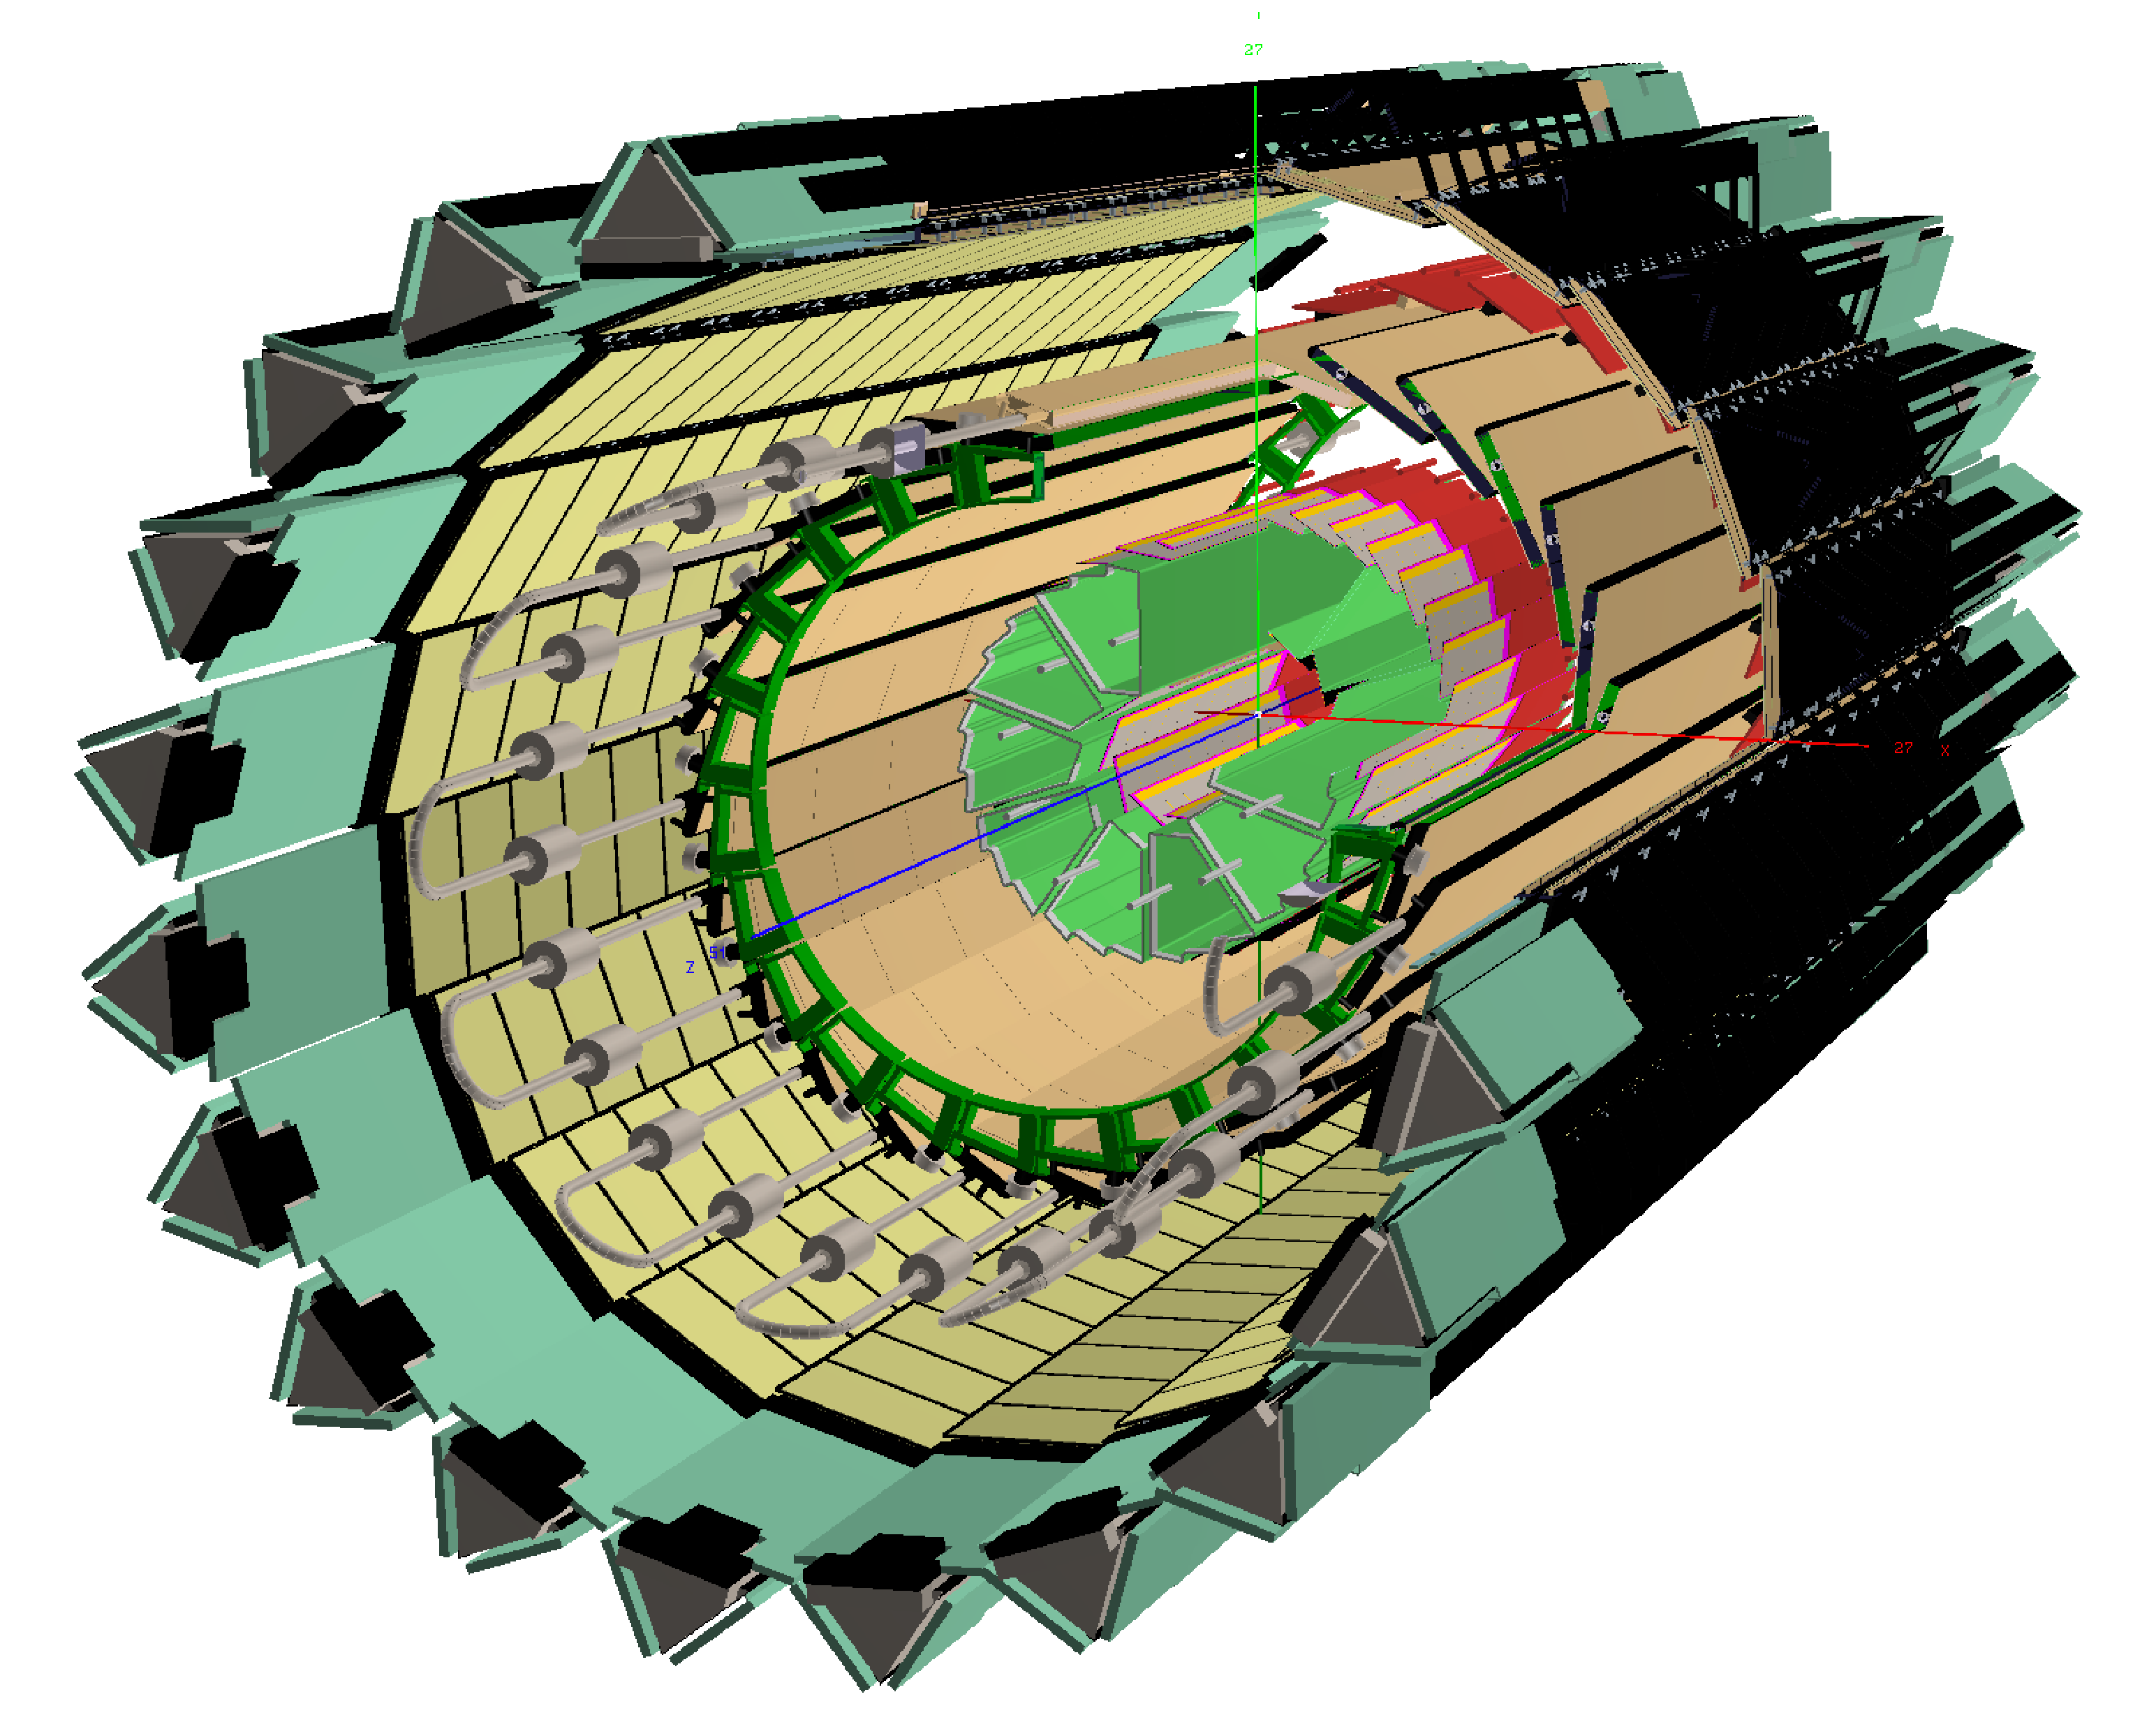
\includegraphics[width=0.5\textwidth]{graphics/hft_cut_away} }

% Labels for hft_cut_away
\rput(5,30){ \rnode{from}{\psframebox{\textbf{SST}, R=22~cm} } }
\rput(5,27){ \pnode{to} }
\ncline[linewidth=0.3,linecolor=redDark,arrowscale=2]{->}{from}{to}

\rput(5,13){ \rnode{from}{\psframebox{\textbf{IST}, R=14~cm} } }
\rput(10,19){ \pnode{to} }
\ncline[linewidth=0.3,linecolor=redDark,arrowscale=2]{->}{from}{to}

\rput(18,14){ \rnode{from}{\psframebox{\textbf{PXL}, R=3~and~8~cm} } }
\rput(14,21){ \pnode{to} }
\ncline[linewidth=0.3,linecolor=redDark,arrowscale=2]{->}{from}{to}


\rput[lb](0.52\textwidth,-0.03\textheight){ 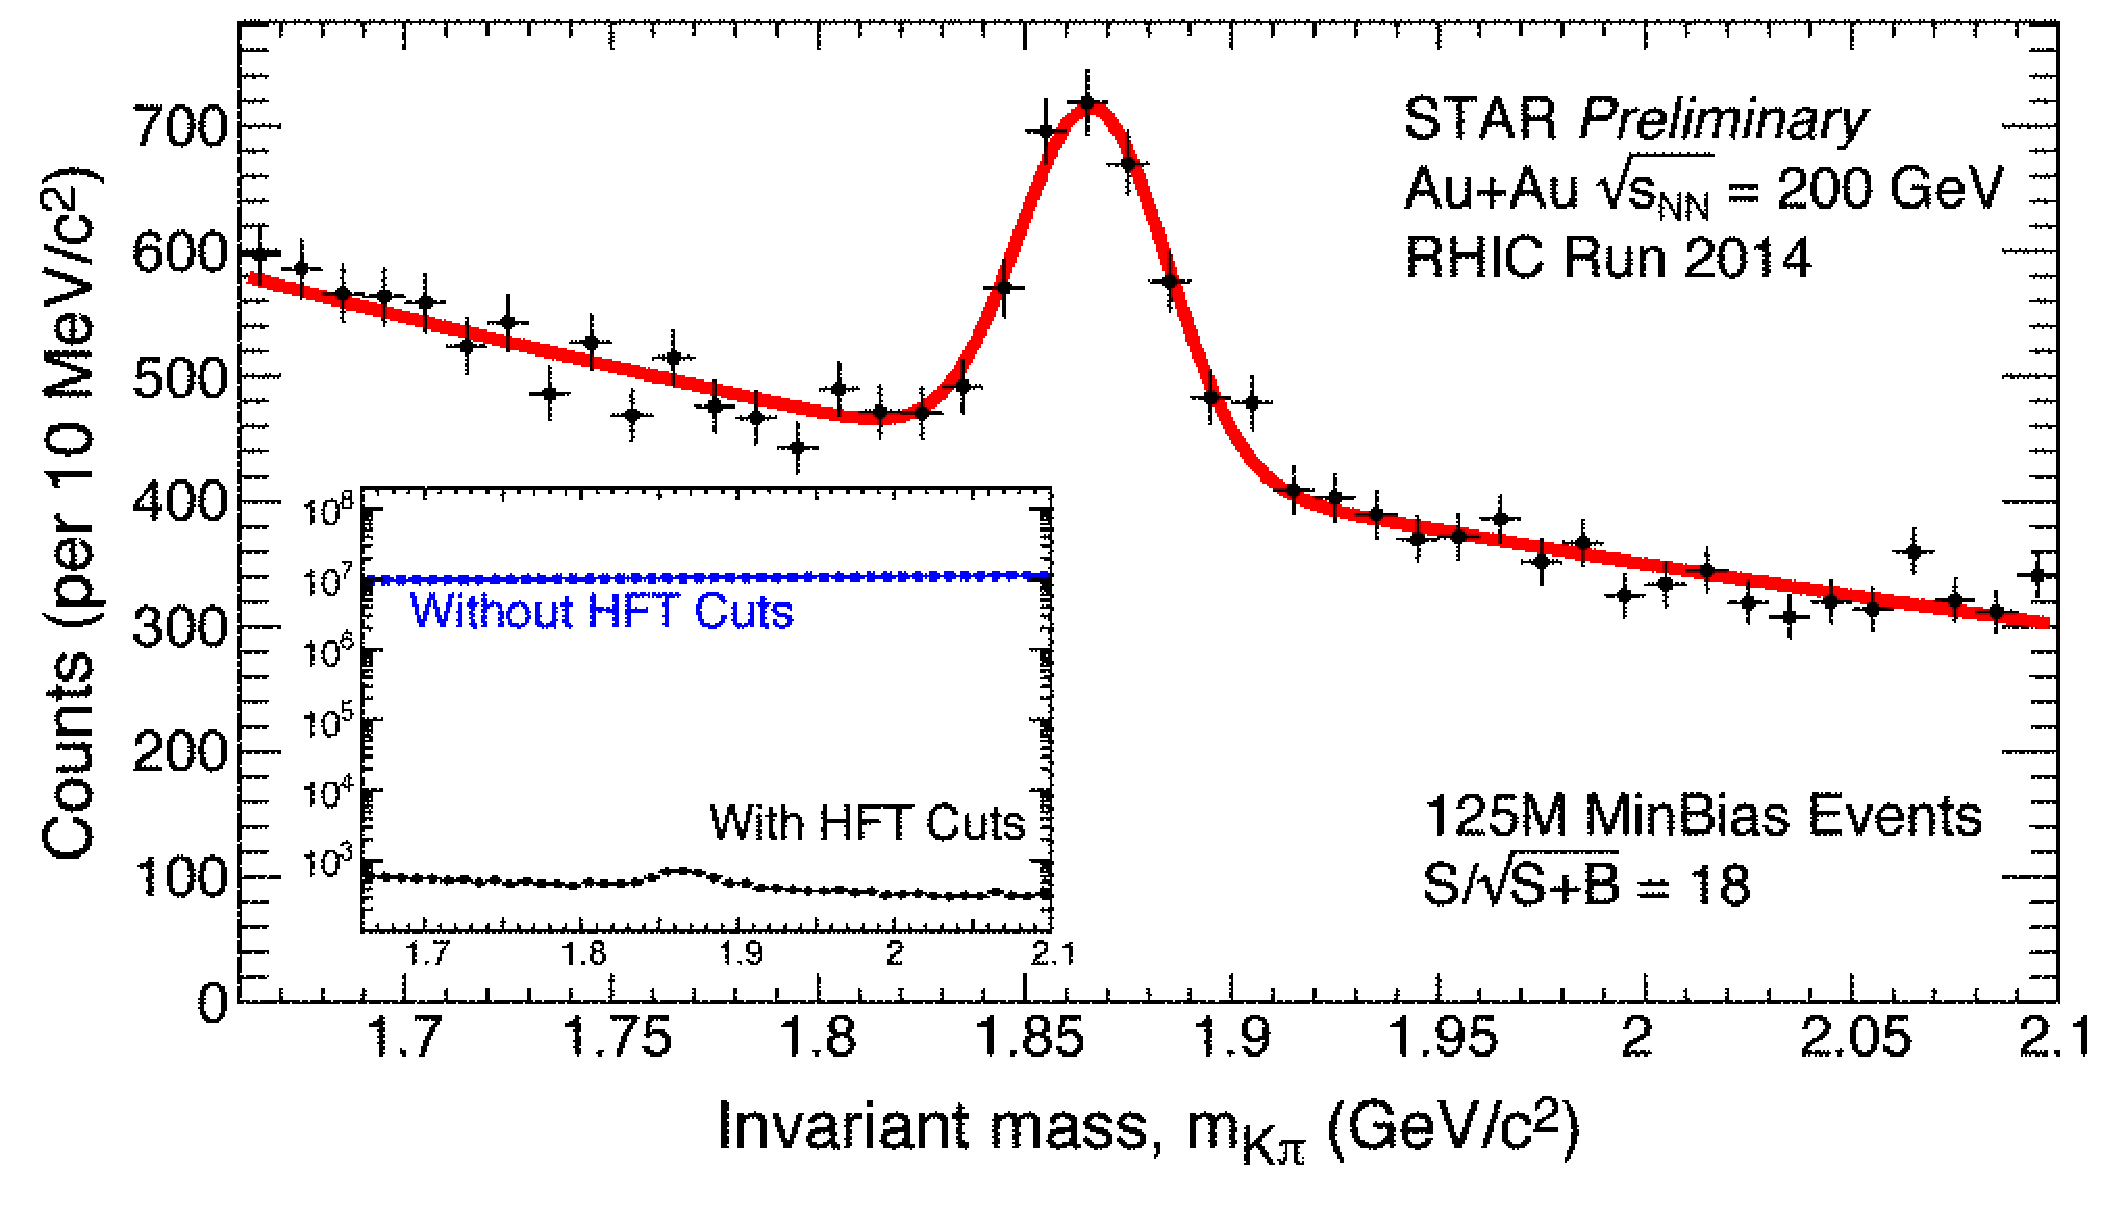
\includegraphics[width=0.45\textwidth]{graphics/PR_D0_official} }

\rput[rb](1.0\textwidth,0.35\textheight){ 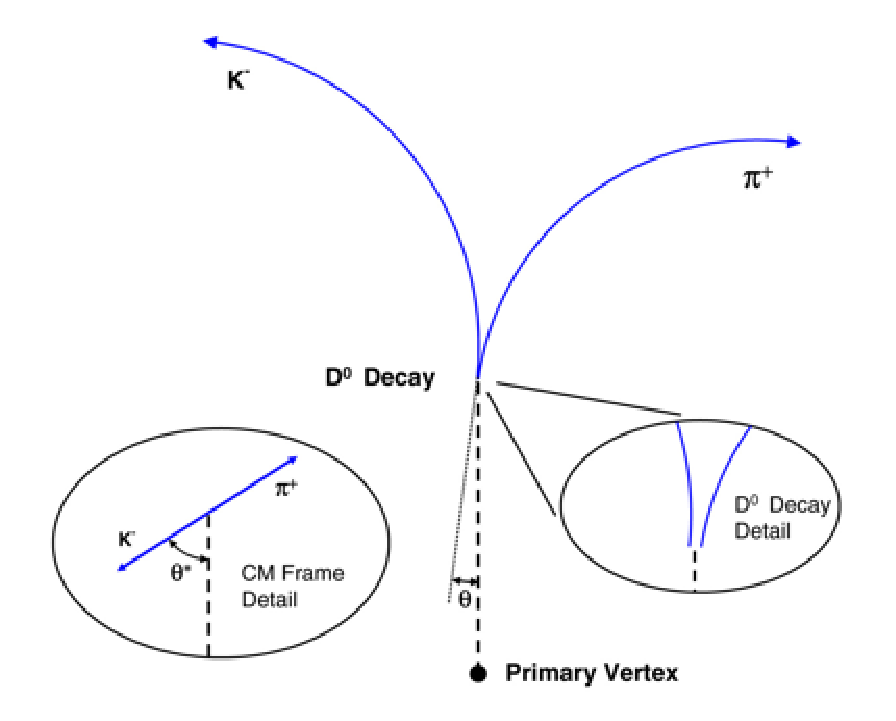
\includegraphics[width=0.2\textwidth]{graphics/D0_decay} }


\rput[l](0.50\textwidth,0.65\textheight) {%
\begin{minipage}{0.50\textwidth}

\raggedright

\begin{list}{\labelitemi}{\setlength{\itemsep}{0mm}
                          \setlength{\topsep}{0mm}}

   \item \textbf{HFT} includes three silicon detecors:\\
		SST, IST, and two layers of PXL

   \item \textbf{HFT} was installed to detect charm decays such as $D^0 \to K \pi$ with small decay length

   \item Direct topological reconstruction of $D$ mesons is done by resolving displaced vertices (50--100~$\mu m$)

   \item \parbox[t]{0.6\linewidth}{\raggedright \textbf{HFT} recorded physics data during three RHIC runs since 2014}

\end{list}

\end{minipage}
}


\rput[r](0.50\textwidth,0.16\textheight) {%
\begin{minipage}{0.48\textwidth}

\raggedright

\begin{list}{\labelitemi}{\setlength{\itemsep}{0mm}
                          \setlength{\topsep}{0mm}}

   \item HFT hits significantly improve resolution of TPC track projections to beam from 1--2~mm to $\sim 30~\mu\text{m}$

   \item \textbf{High precision tracking with HFT prompted us to revisit STAR tracking and vertexing algorithms}

\end{list}

\end{minipage}
}


%\psgrid[gridlabels=0.7,subgriddiv=0, griddots=3](1,-1)(0,-3)(\textwidth,\textheight)

\end{pspicture}
%}}}



%===============================================================================
\myfoilhead{-30mm}{Vertex Reconstruction Algorithms at STAR}
%{{{

\noindent
\begin{pspicture}(0,0)(\textwidth,\textheight)


\rput[lb](0.52\textwidth,0.55\textheight){ 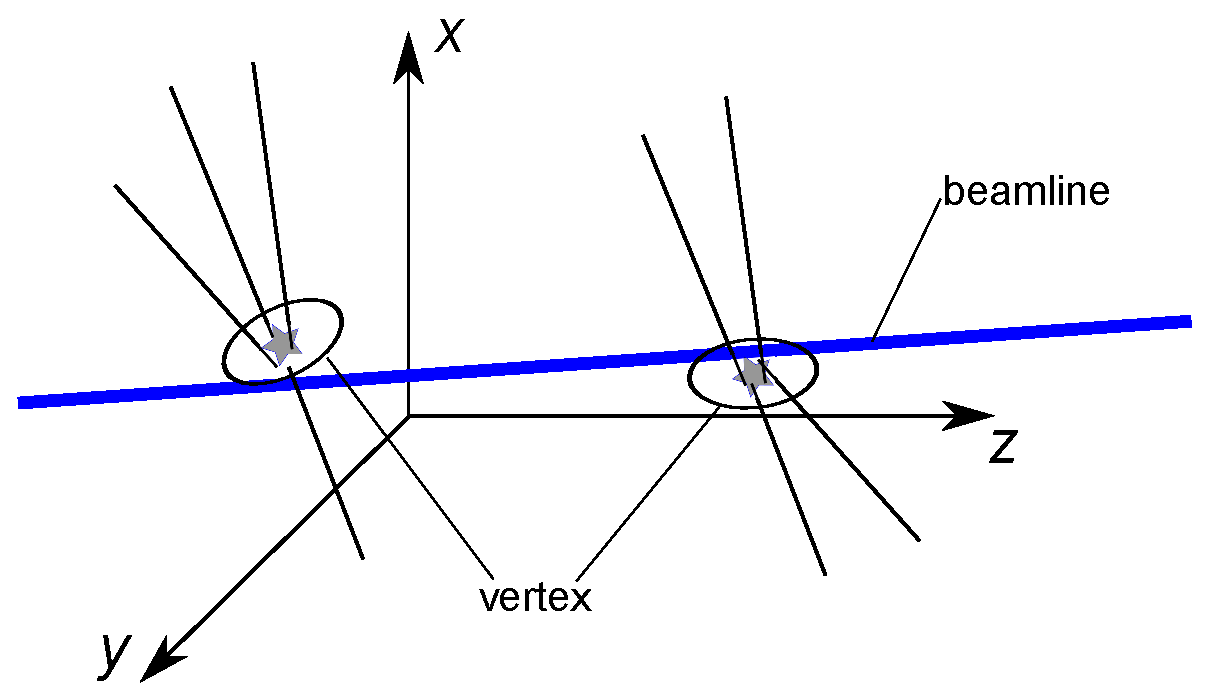
\includegraphics[width=0.45\textwidth]{graphics/beamline_vertex_3d} }
\rput[t](0.75\textwidth,0.54\textheight){ 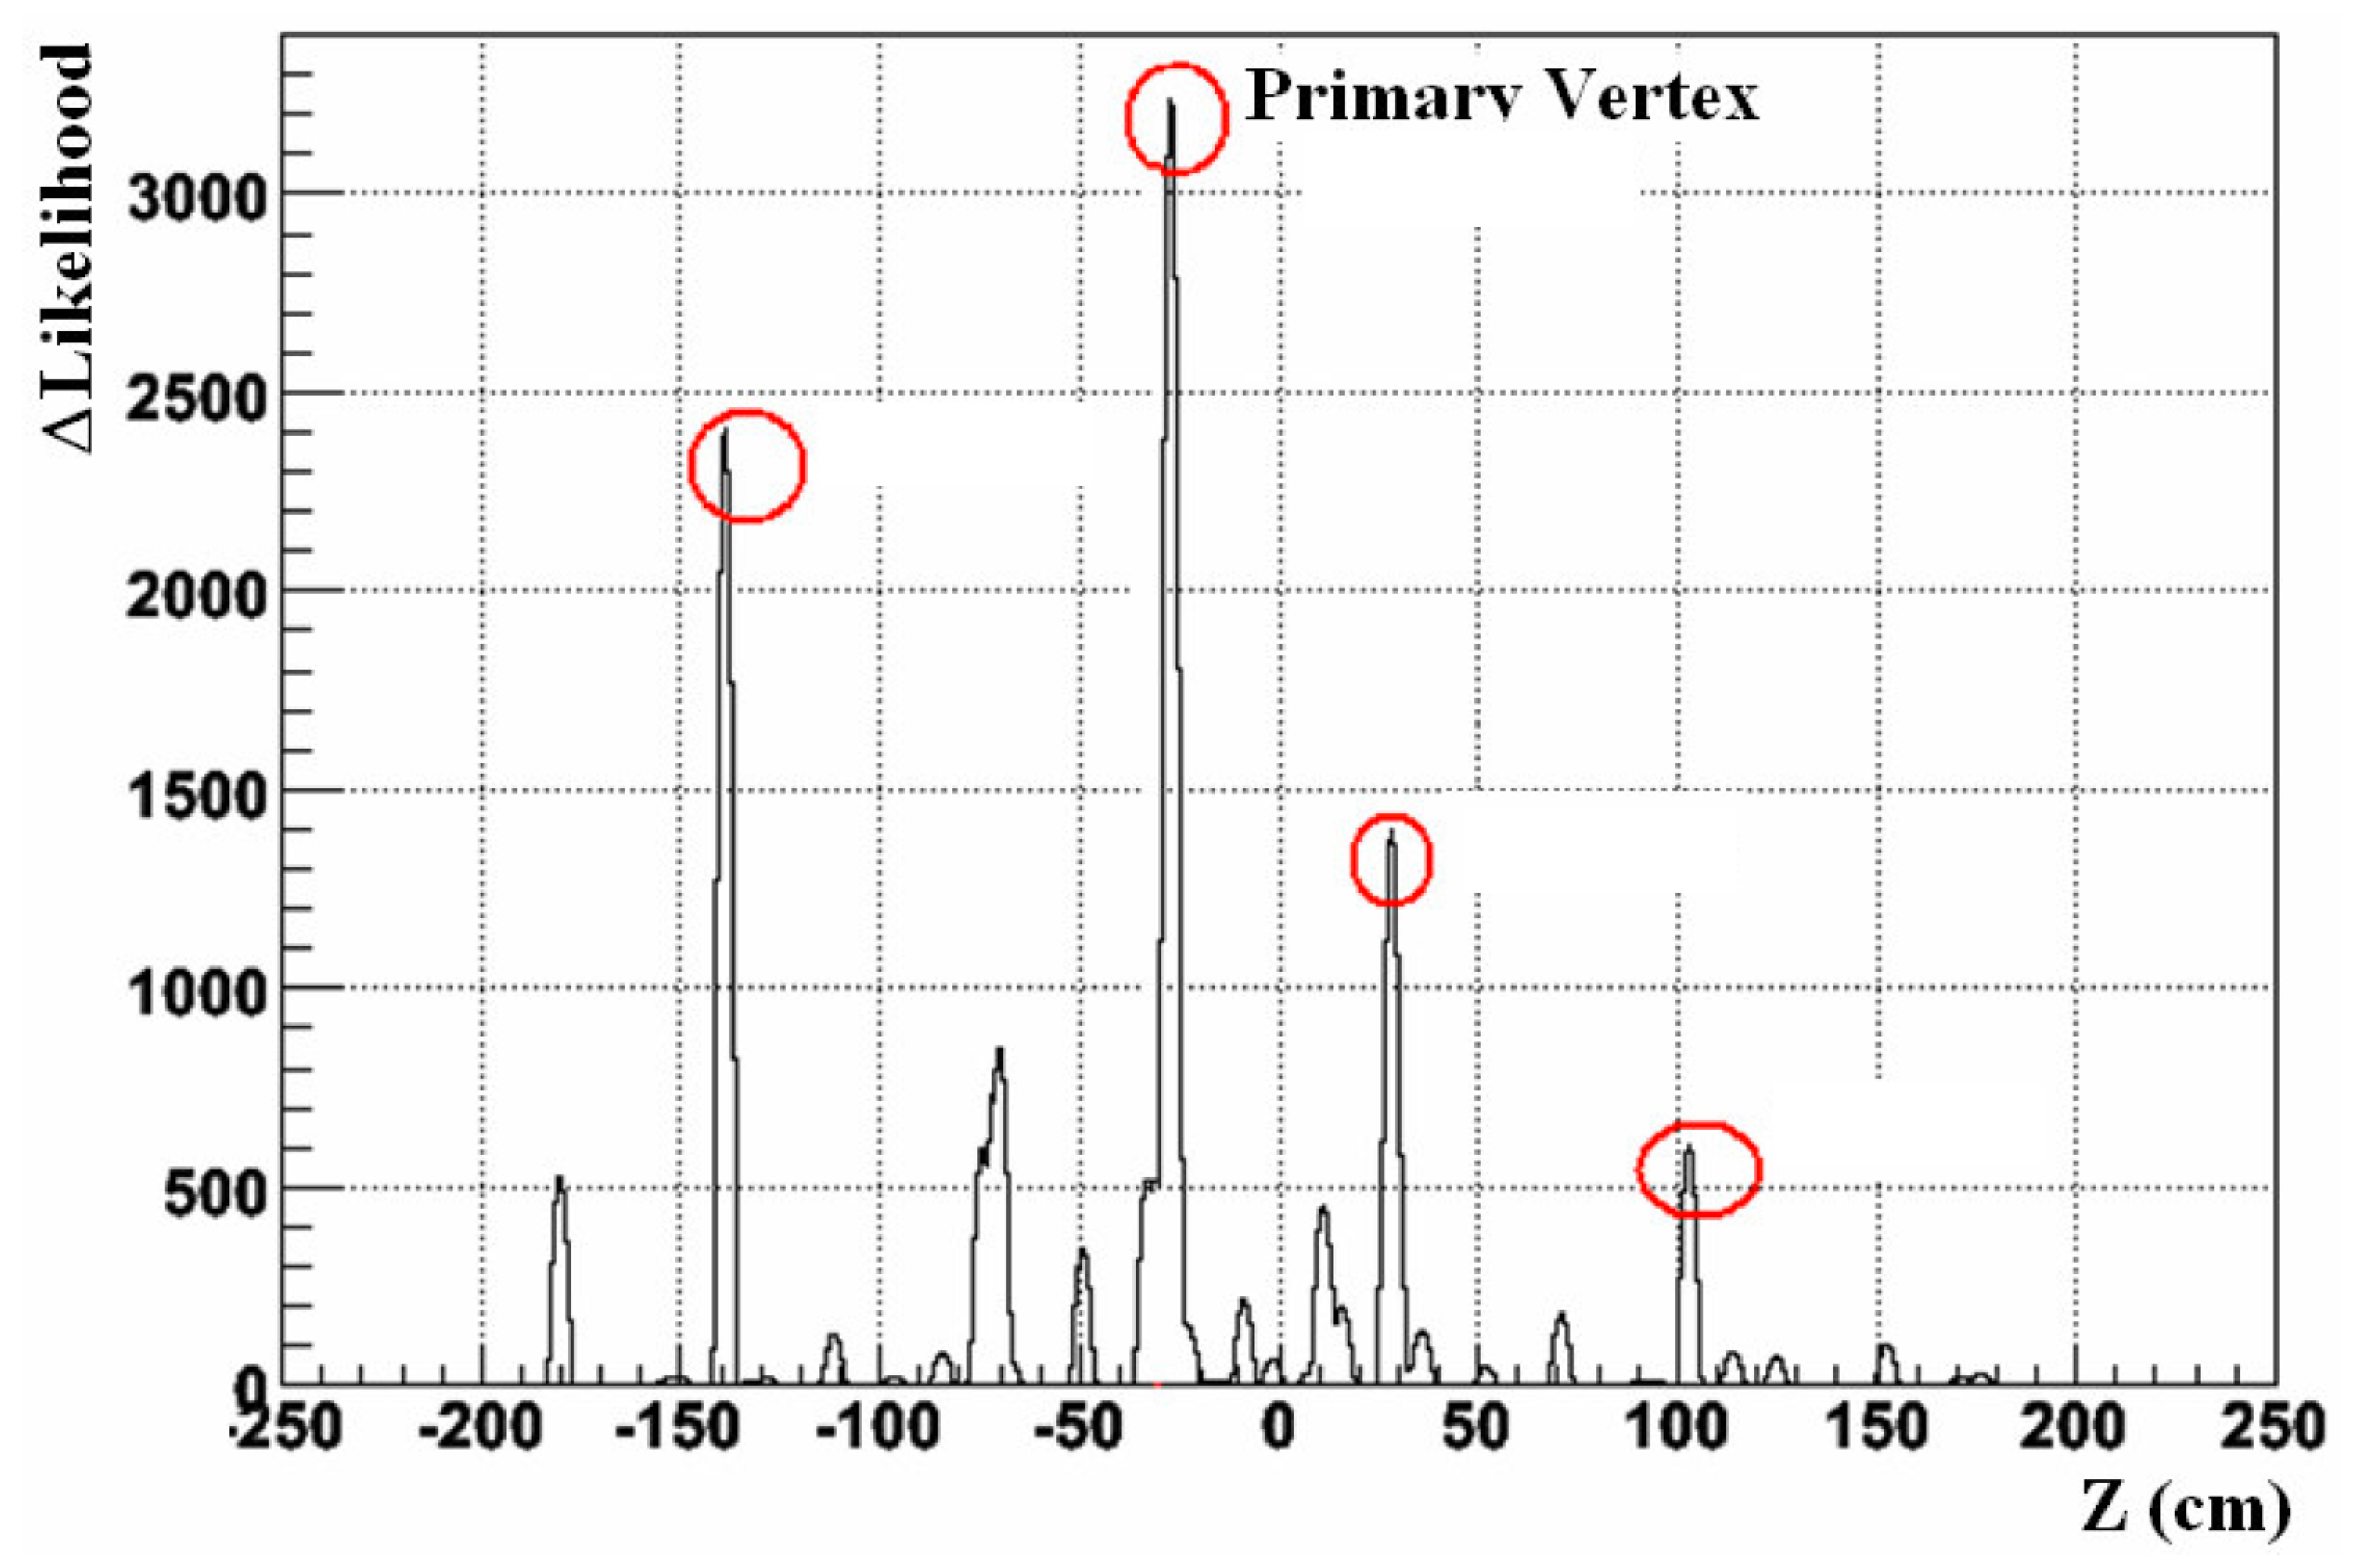
\includegraphics[width=0.40\textwidth]{graphics/ppv_likelihood} }


\rput[rt](0.52\textwidth,0.90\textheight) {%
\begin{minipage}{0.50\textwidth}

\raggedright

\begin{list}{\labelitemi}{\setlength{\itemsep}{0mm}
                          \setlength{\topsep}{0mm}}

   \item Two vertex reconstruction algorithms:\\
      \textbf{Pile-up Proof Vertexer} (PPV)\\
      \textbf{Minuit-based Vertex Finder} (MinuitVF)

   \begin{list}{\labelitemii}{\setlength{\itemsep}{0mm}
                              \setlength{\topsep}{0mm}}

      \item {\footnotesize STAR is also evaluating an adaptive vertexer, KFV, based on Kalman Filter}

   \end{list}

   \small


   \item \textbf{PPV} and \textbf{MinuitVF} are traditional algorithms with dominating seeding/finding stage

   \begin{list}{\labelitemii}{\setlength{\itemsep}{2mm}
                              \setlength{\topsep}{0mm}}

      \item Rely on similar track preselection

      \item Seeding performed in 1D along the beam with predetermined initial binning

      \item \textbf{PPV} and \textbf{MinuitVF} reconstruct different
      event topologies: $\mathbf{pp}$ and \textbf{heavy ion} collisions respectively

   \end{list}

\end{list}

\end{minipage}
}

\rput[b](0.48\textwidth,-1.2\unitlength) {%
\begin{minipage}{0.60\textwidth}

\raggedright

\begin{list}{\labelitemi}{\setlength{\itemsep}{0mm}
                          \setlength{\topsep}{0mm}}

   \item A few areas for improvements have been identified:

   \begin{list}{\labelitemii}{\setlength{\itemsep}{0mm}
                              \setlength{\topsep}{-5mm}}

      \item \textbf{PPV} is lacking the final fitting stage

      \item No beamline uncertainties utilized by either vertexer

   \end{list}

\end{list}

\end{minipage}
}


%\psgrid[gridlabels=0.7,subgriddiv=0, griddots=3](1,-1)(0,-3)(\textwidth,\textheight)

\end{pspicture}
%}}}



%===============================================================================
\myfoilhead{-30mm}{Dealing with Pile-up Tracks: Vertex Ranking}
%{{{

\noindent
\begin{pspicture}(0,0)(\textwidth,\textheight)

\rput[l](0.01\textwidth,0.75\textheight){ 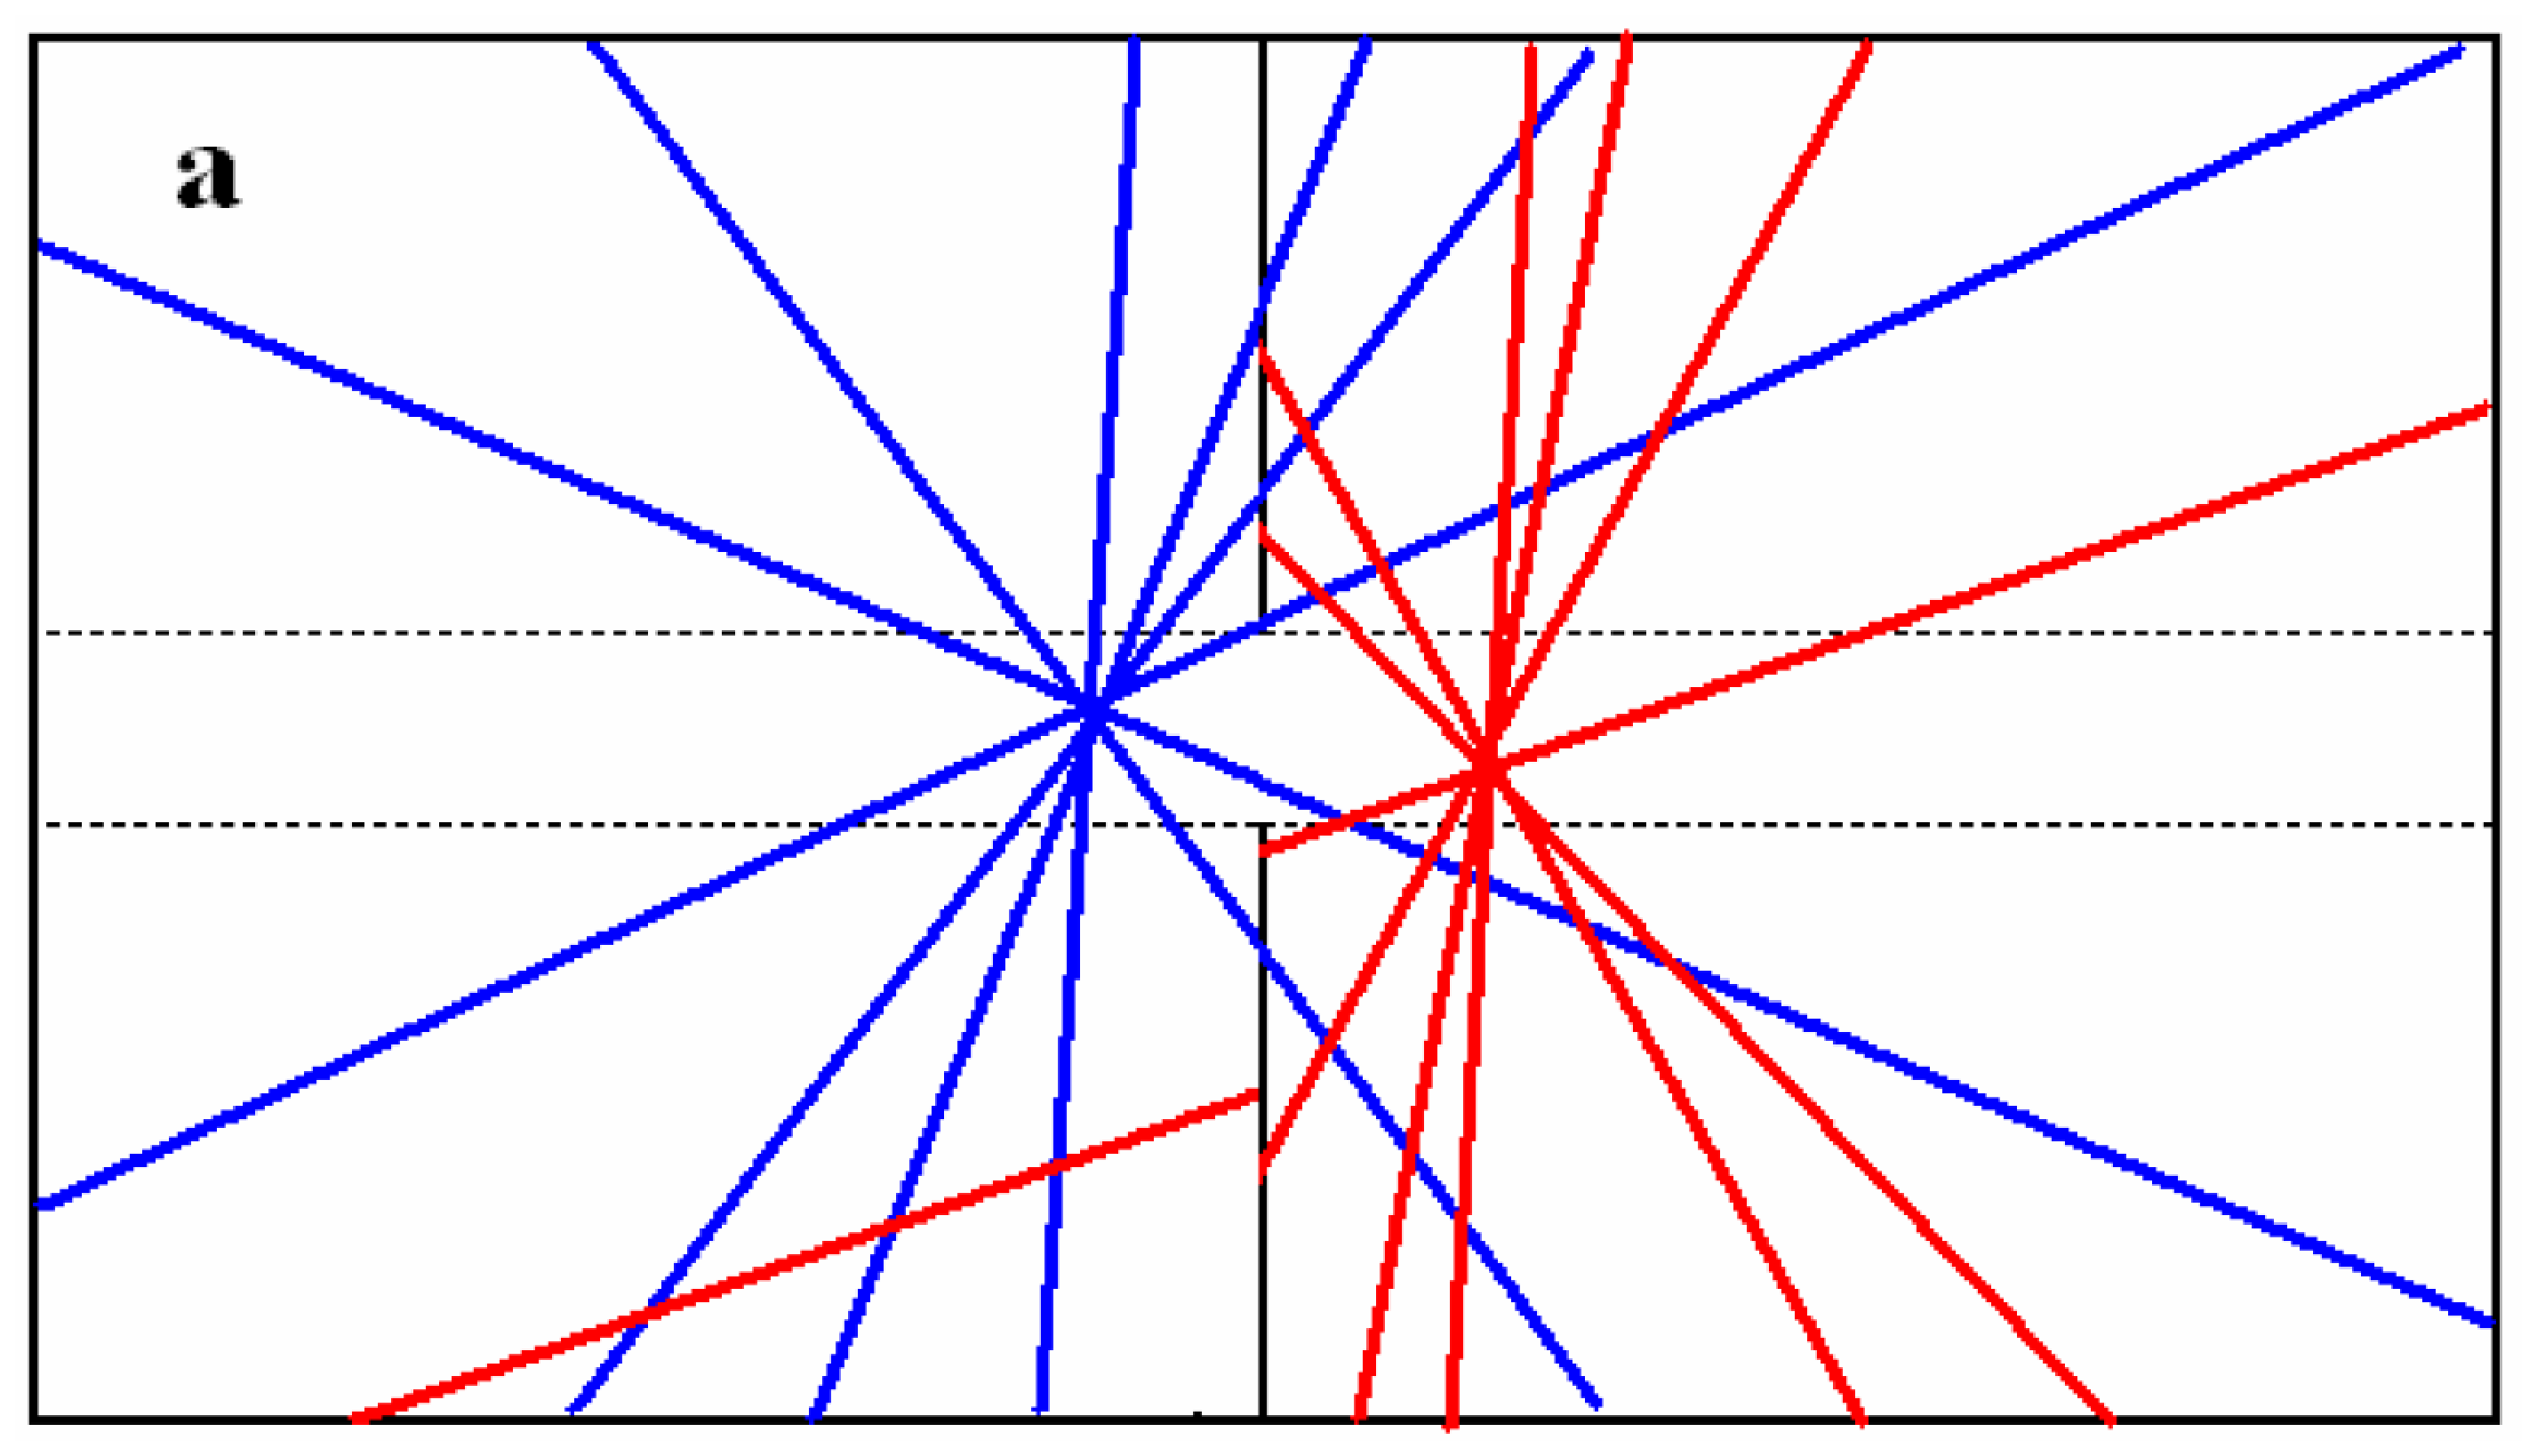
\includegraphics[height=0.25\textheight]{graphics/split_tracks_a} }
\rput[l](0.01\textwidth,0.48\textheight){ 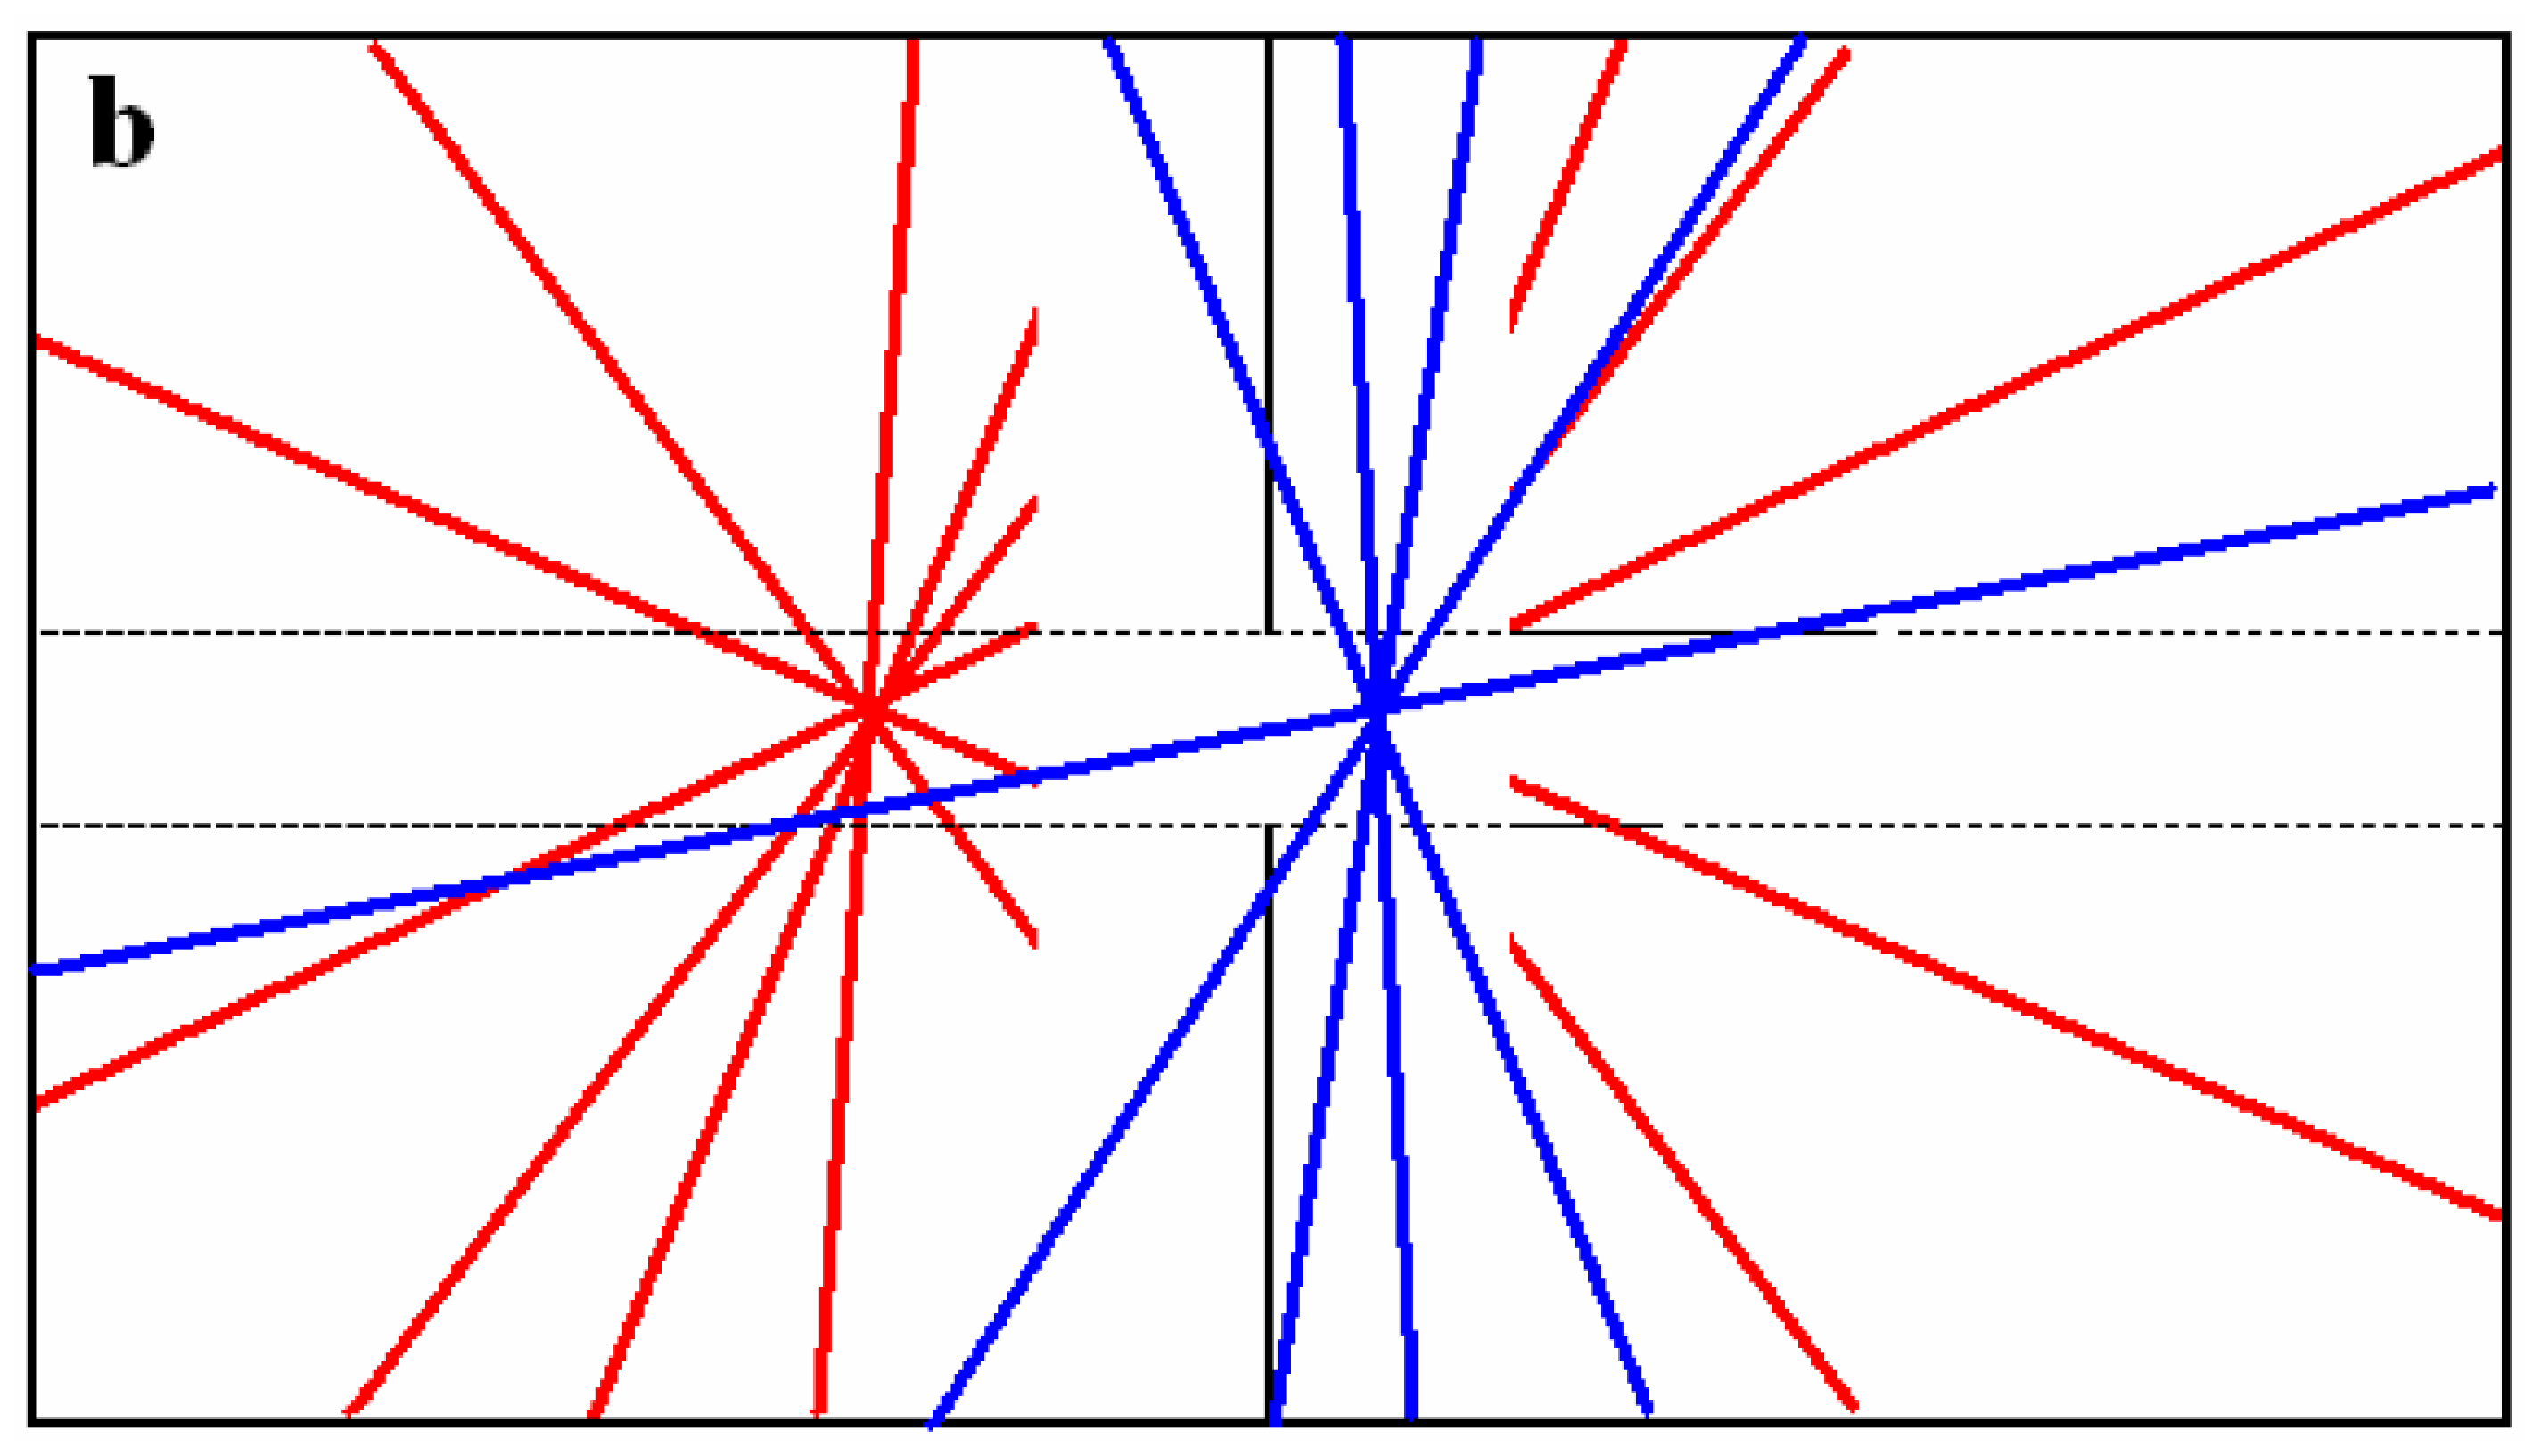
\includegraphics[height=0.25\textheight]{graphics/split_tracks_b} }
\rput[l](0.01\textwidth,0.21\textheight){ 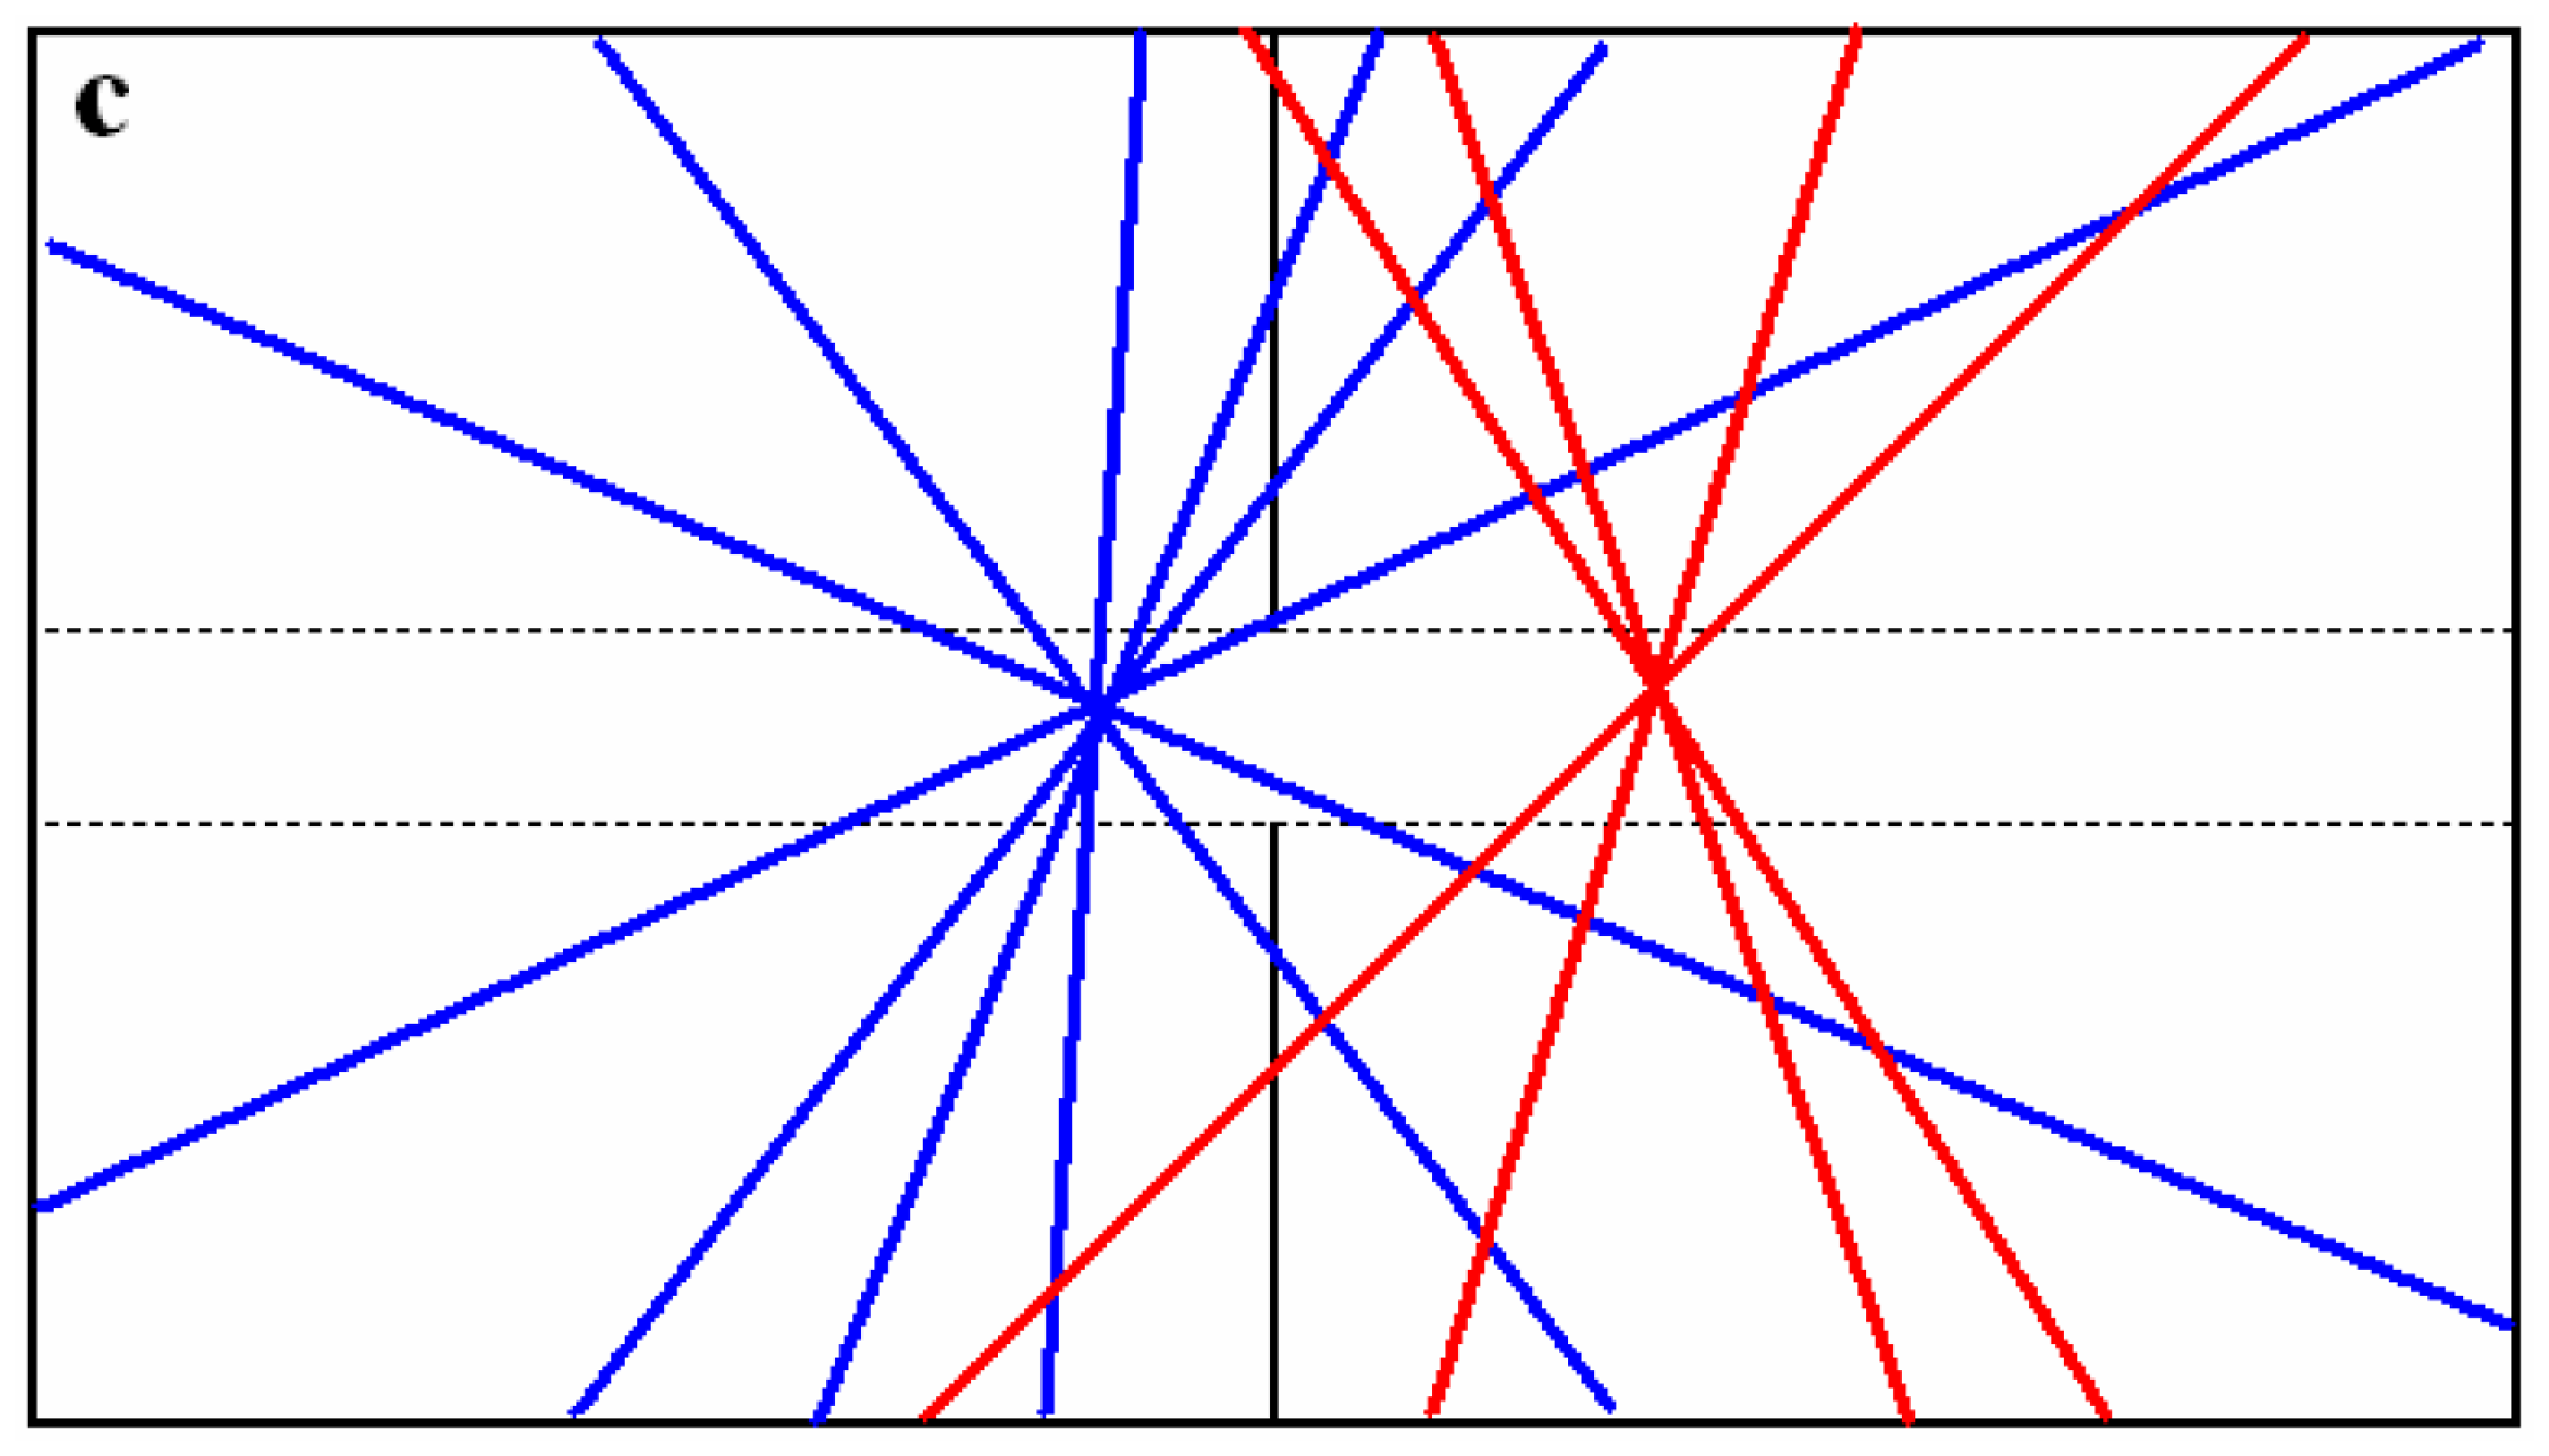
\includegraphics[height=0.25\textheight]{graphics/split_tracks_c} }

\rput[r](1\textwidth,0.38\textheight){ 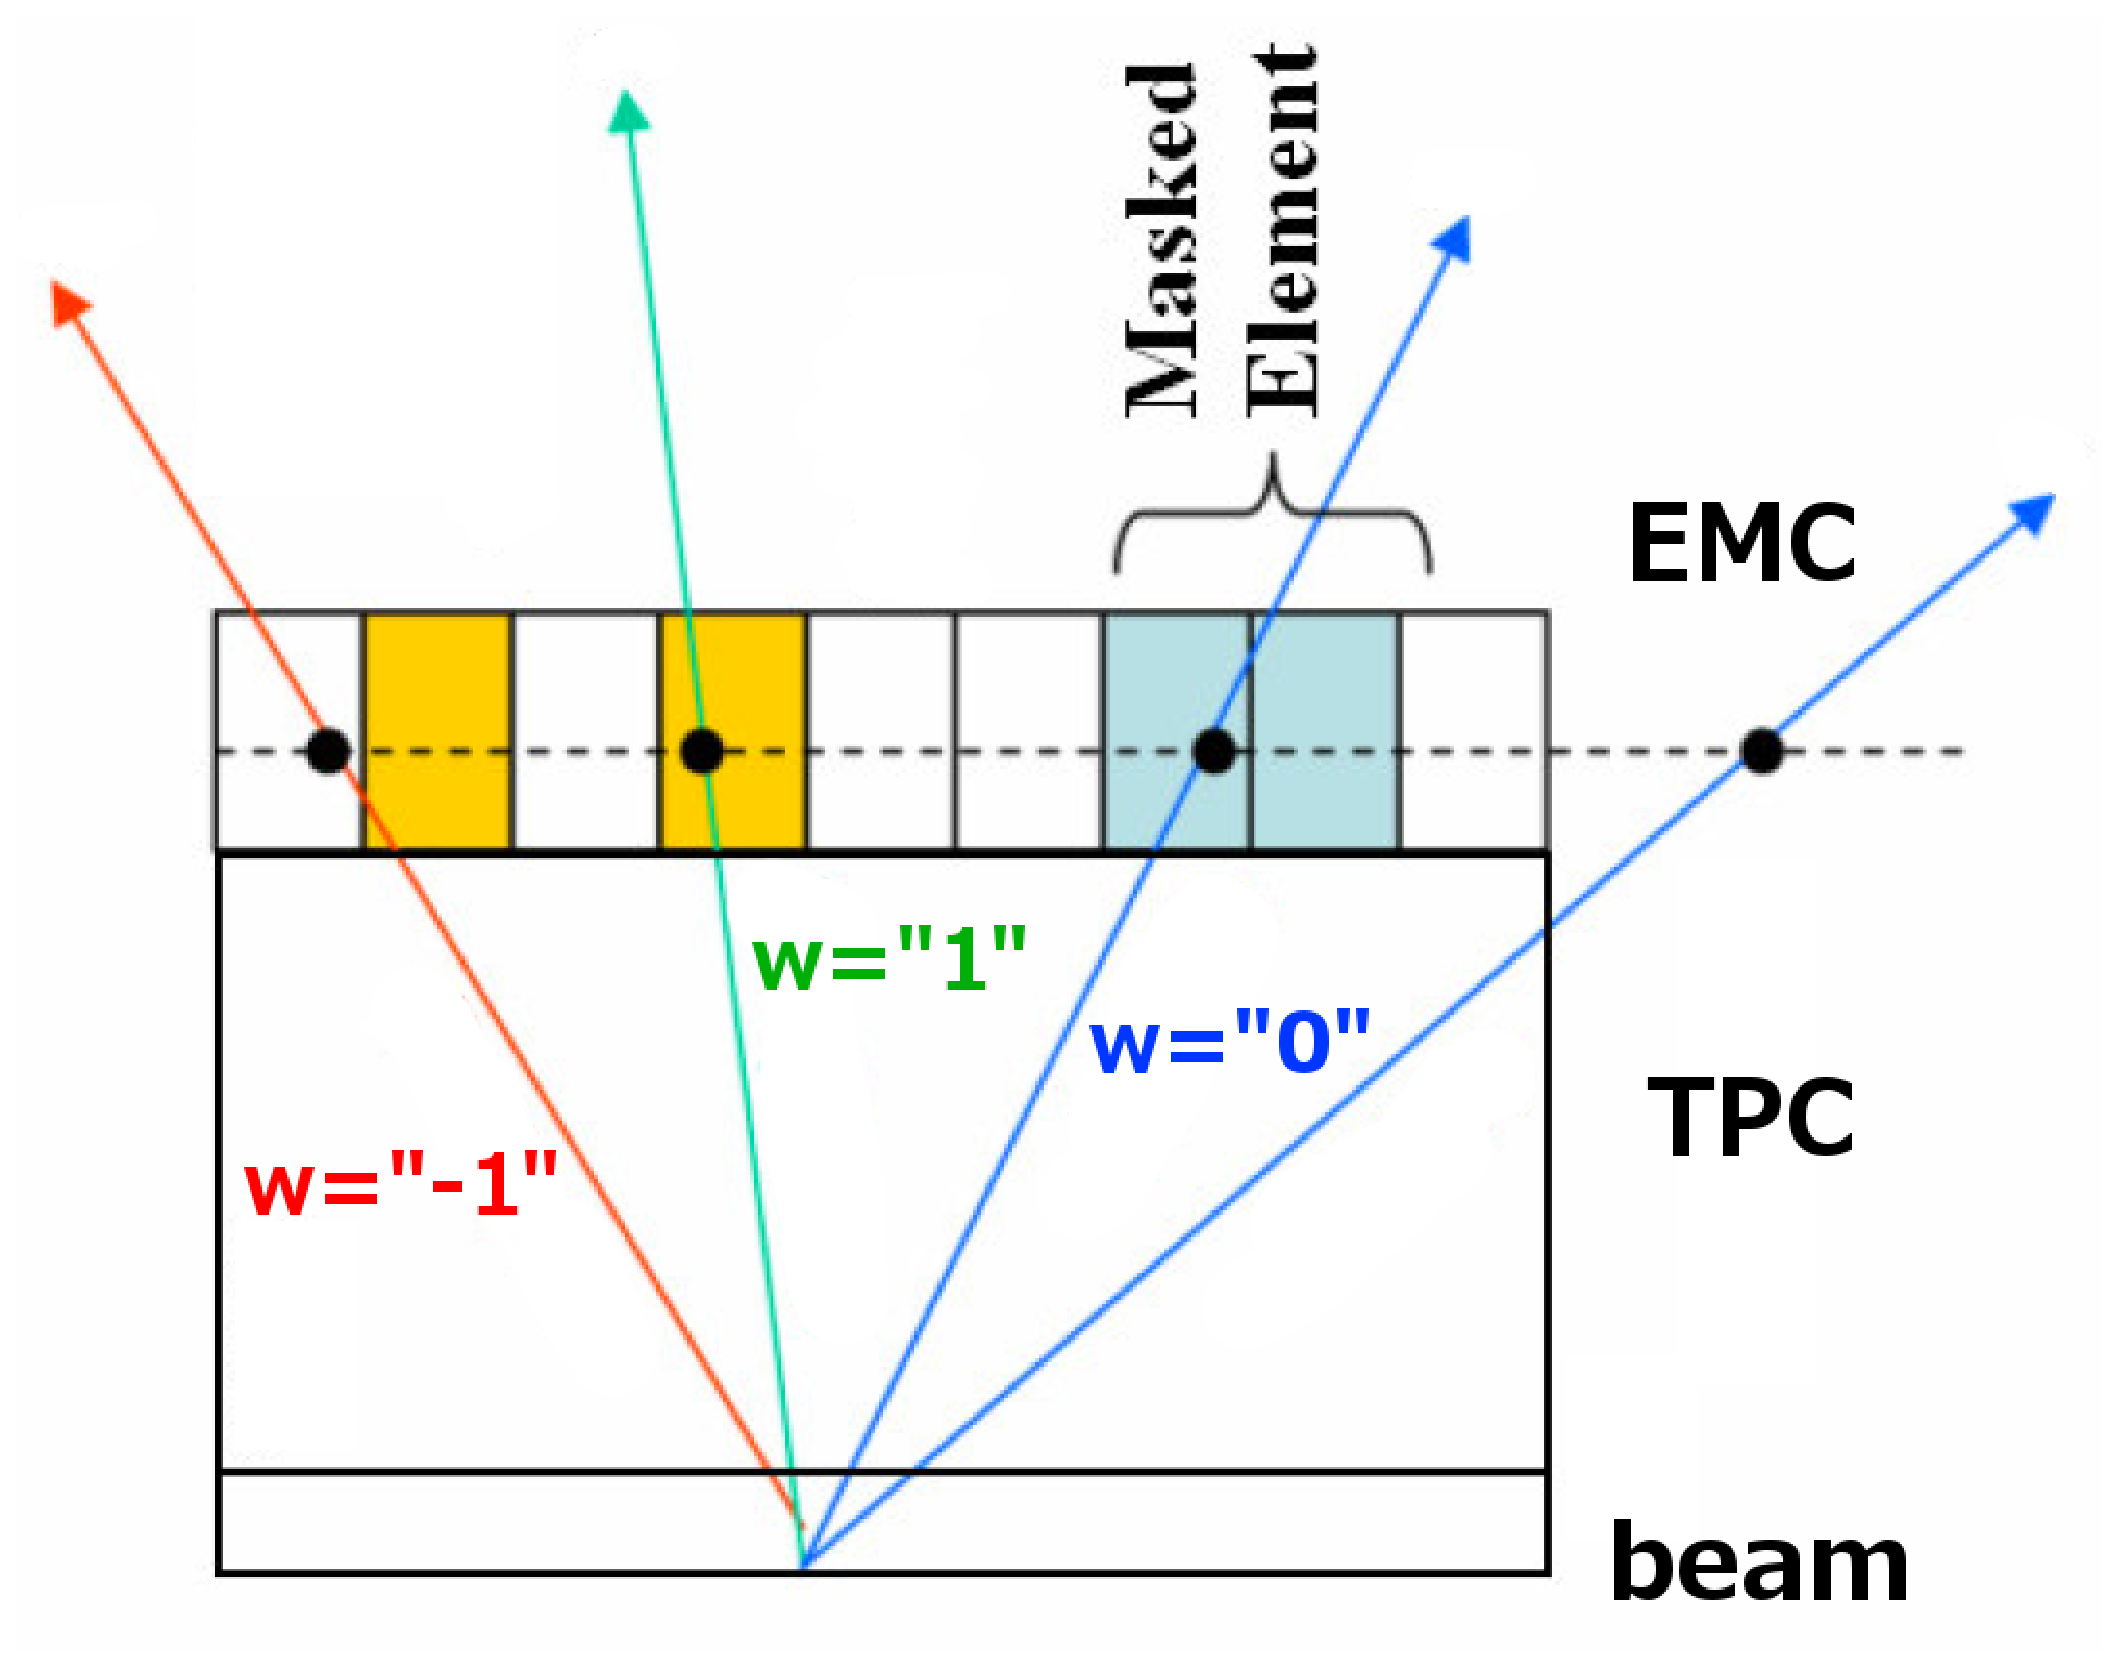
\includegraphics[width=0.35\textwidth]{graphics/ppv_vertex_track_weights} }


\rput[l](0.32\textwidth,0.48\textheight) {%
\begin{minipage}{0.67\textwidth}

\raggedright

\begin{list}{\labelitemi}{\setlength{\itemsep}{3mm}
                          \setlength{\topsep}{0mm}}

   \item 400 bunch crossings per acquired STAR TPC event\\
      $\mathbf{\Rightarrow}$ pile-up tracks

   \item When pile-up collisions occur before or after the triggered event the tracks in STAR TPC appear to be split

   \item Tracks are given weights based on the probability that they originated in the collision firing the trigger

   \parbox{0.44\textwidth}{
   \raggedright
   \begin{list}{\labelitemii}{\setlength{\itemsep}{3mm}
                              \setlength{\topsep}{0mm}}

      \item Fast non-tracking detectors, e.g. EM calorimeter and Time of Flight detector, employed to mitigate the effect

      \item Total weight is used in ranking tracks and vertices

   \end{list}
   }

   \item Identification of pile-up vertices produced in the same bunch crossing
   as the triggered one is left to analyzers 

\end{list}

\end{minipage}
}


\rput(0.50\textwidth,-1\unitlength){ \psframebox{\footnotesize CHEP 2009 proceedings, J. Phys. conf. Ser. 219 032020} }


%\psgrid[gridlabels=0.7,subgriddiv=0, griddots=3](1,-1)(0,-3)(\textwidth,\textheight)

\end{pspicture}
%}}}



%===============================================================================
\myfoilhead{-30mm}{Dealing with Pile-up Tracks: Robust Potential}
%{{{

\noindent
\begin{pspicture}(0,0)(\textwidth,\textheight)

\rput[r](0.95\textwidth,0.82\textheight){ 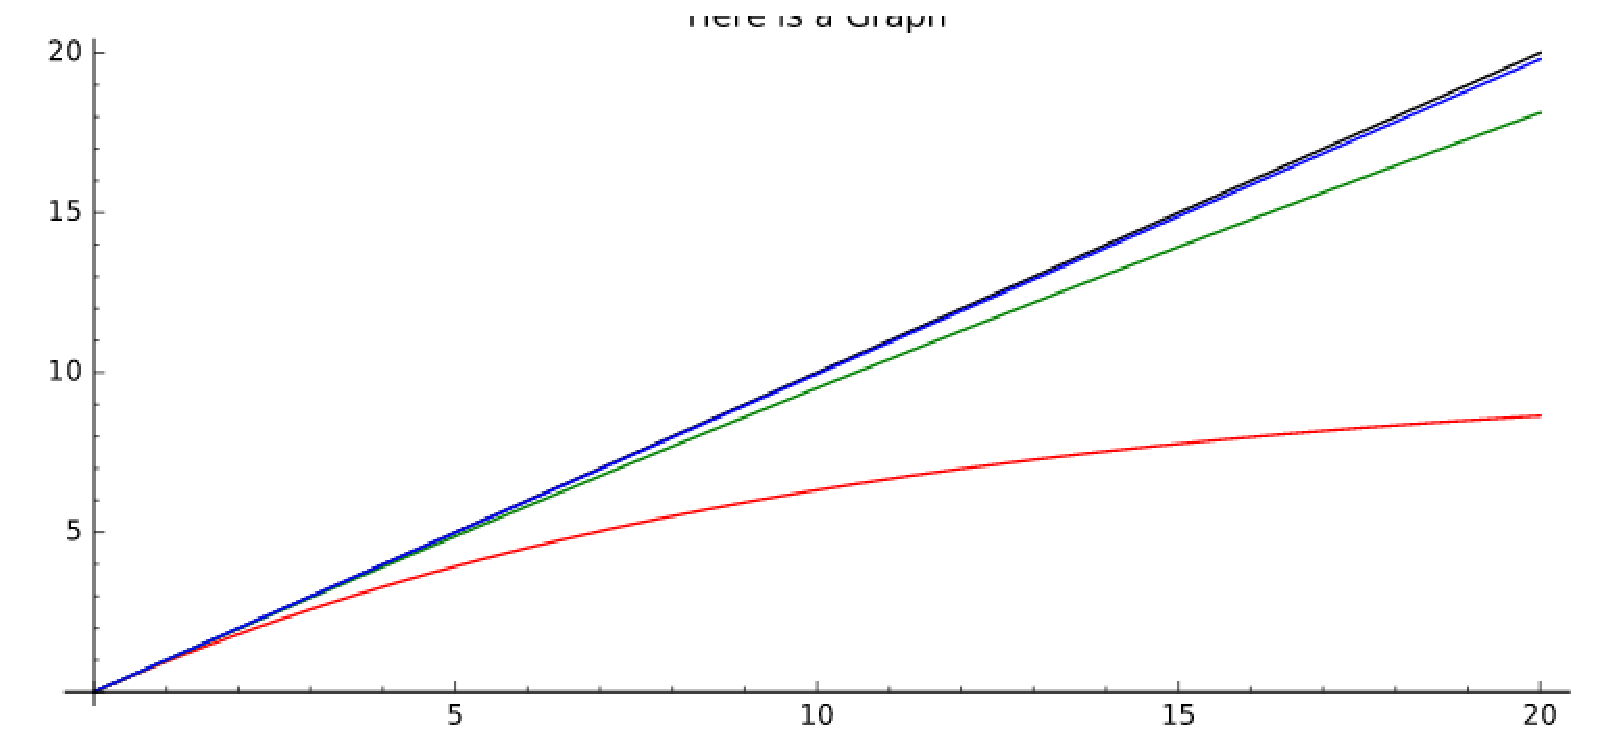
\includegraphics[height=0.20\textheight]{graphics/robust_potential} }
\rput[r](1\textwidth,0.60\textheight){ 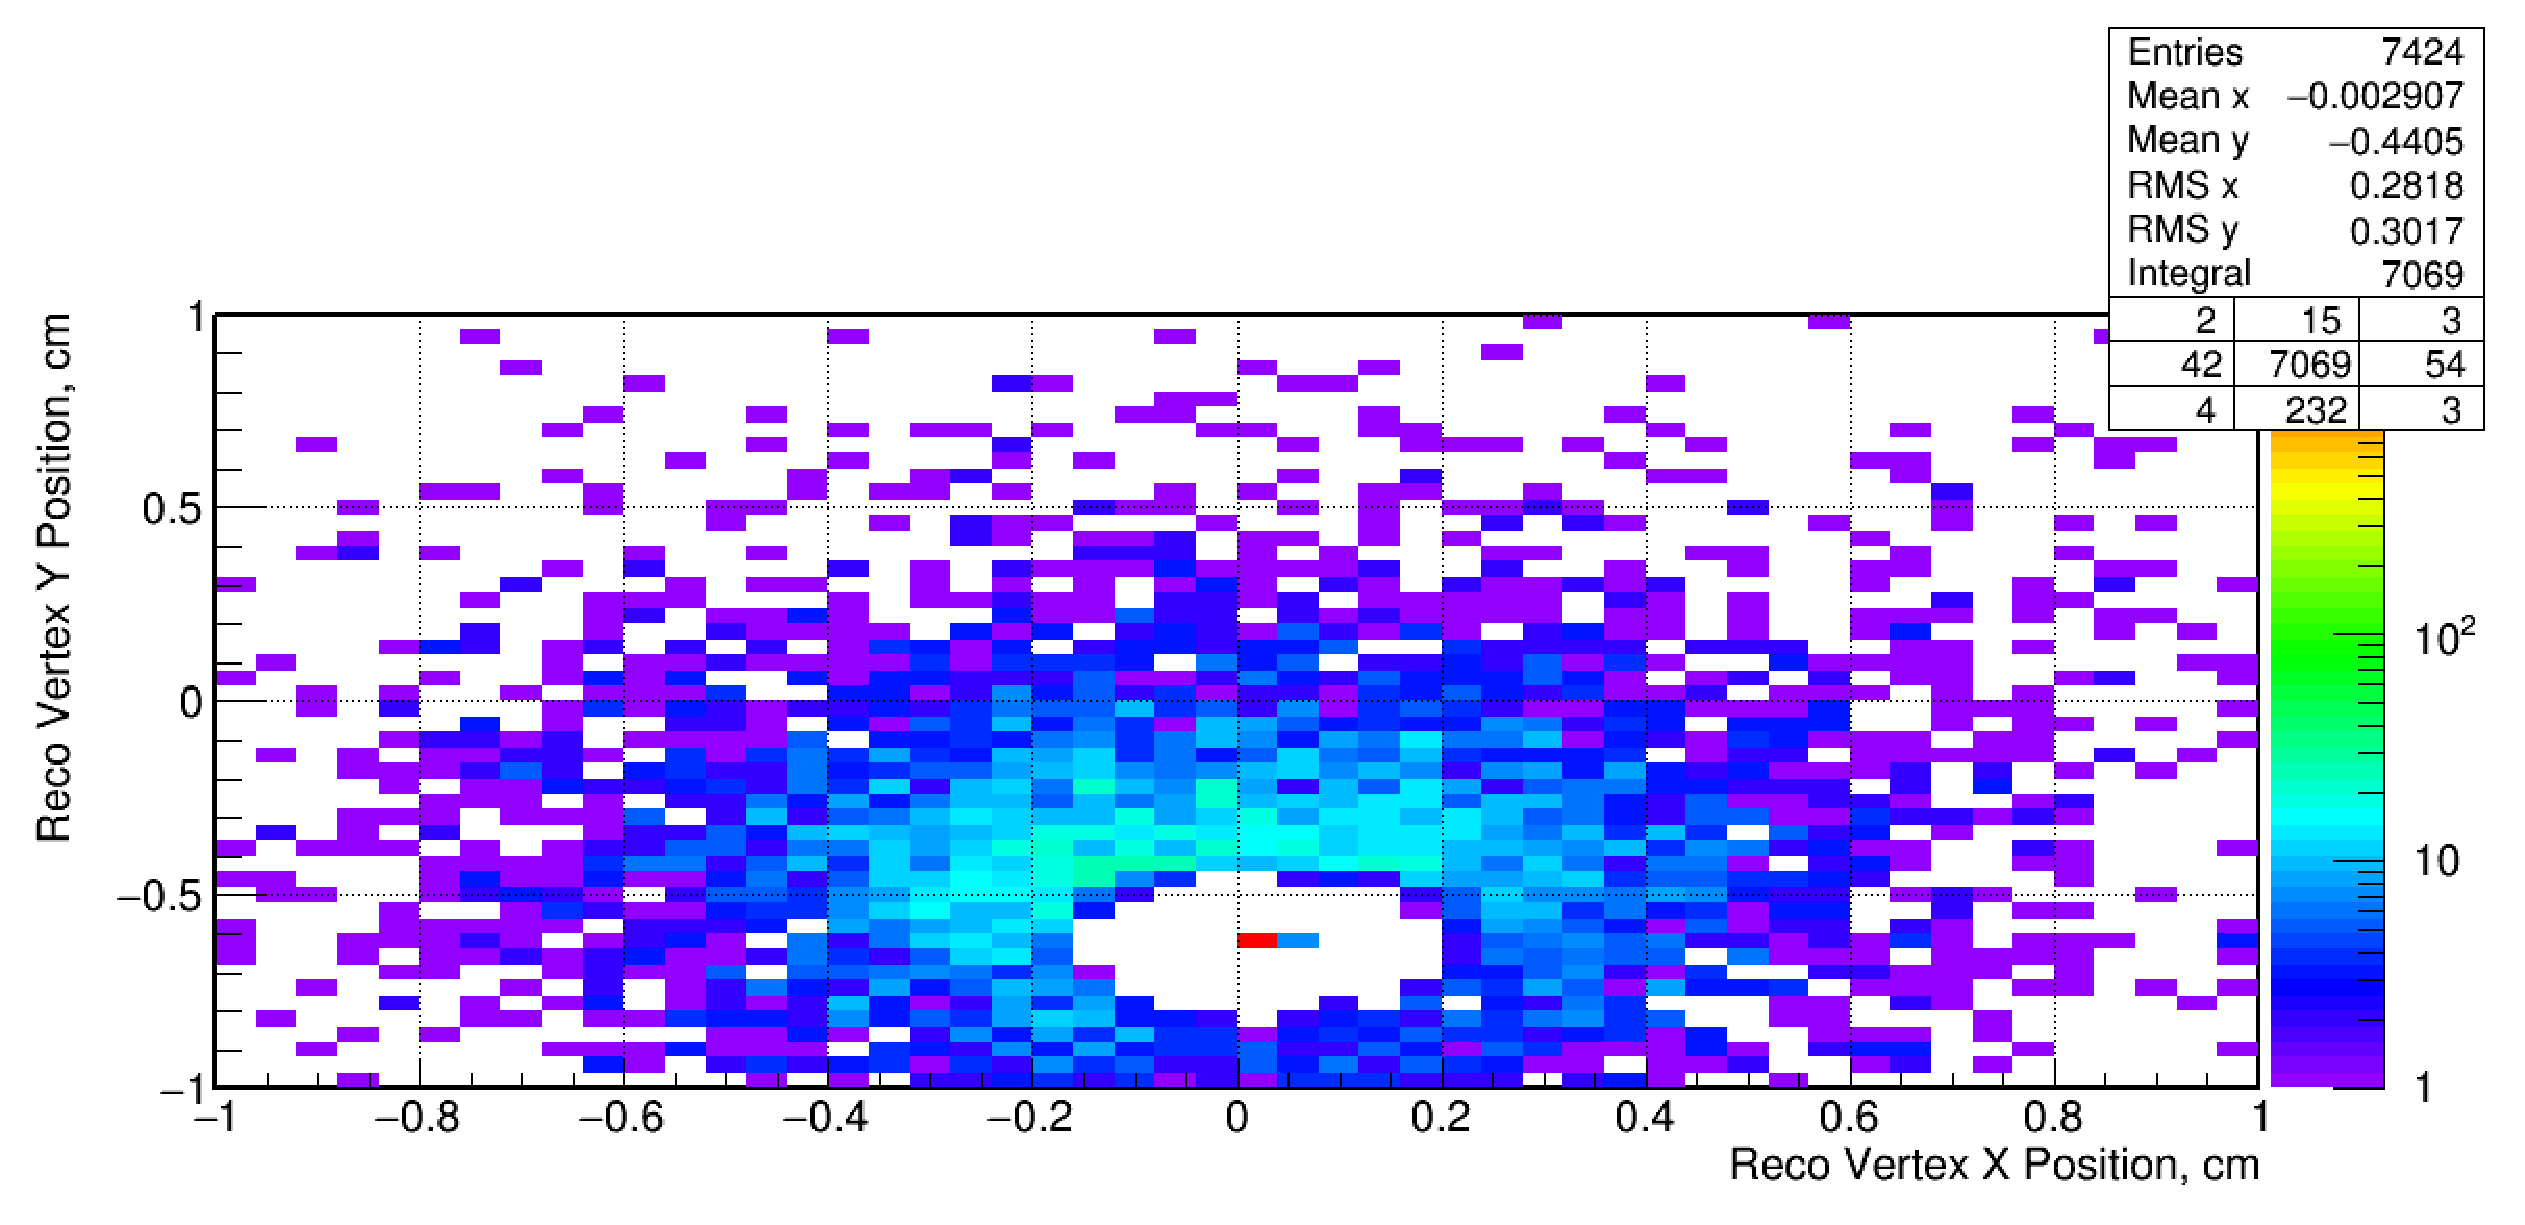
\includegraphics[height=0.25\textheight]{graphics/wemb_PPV_bl3D_s50_hVertexXvY} }
\rput[r](1\textwidth,0.35\textheight){ 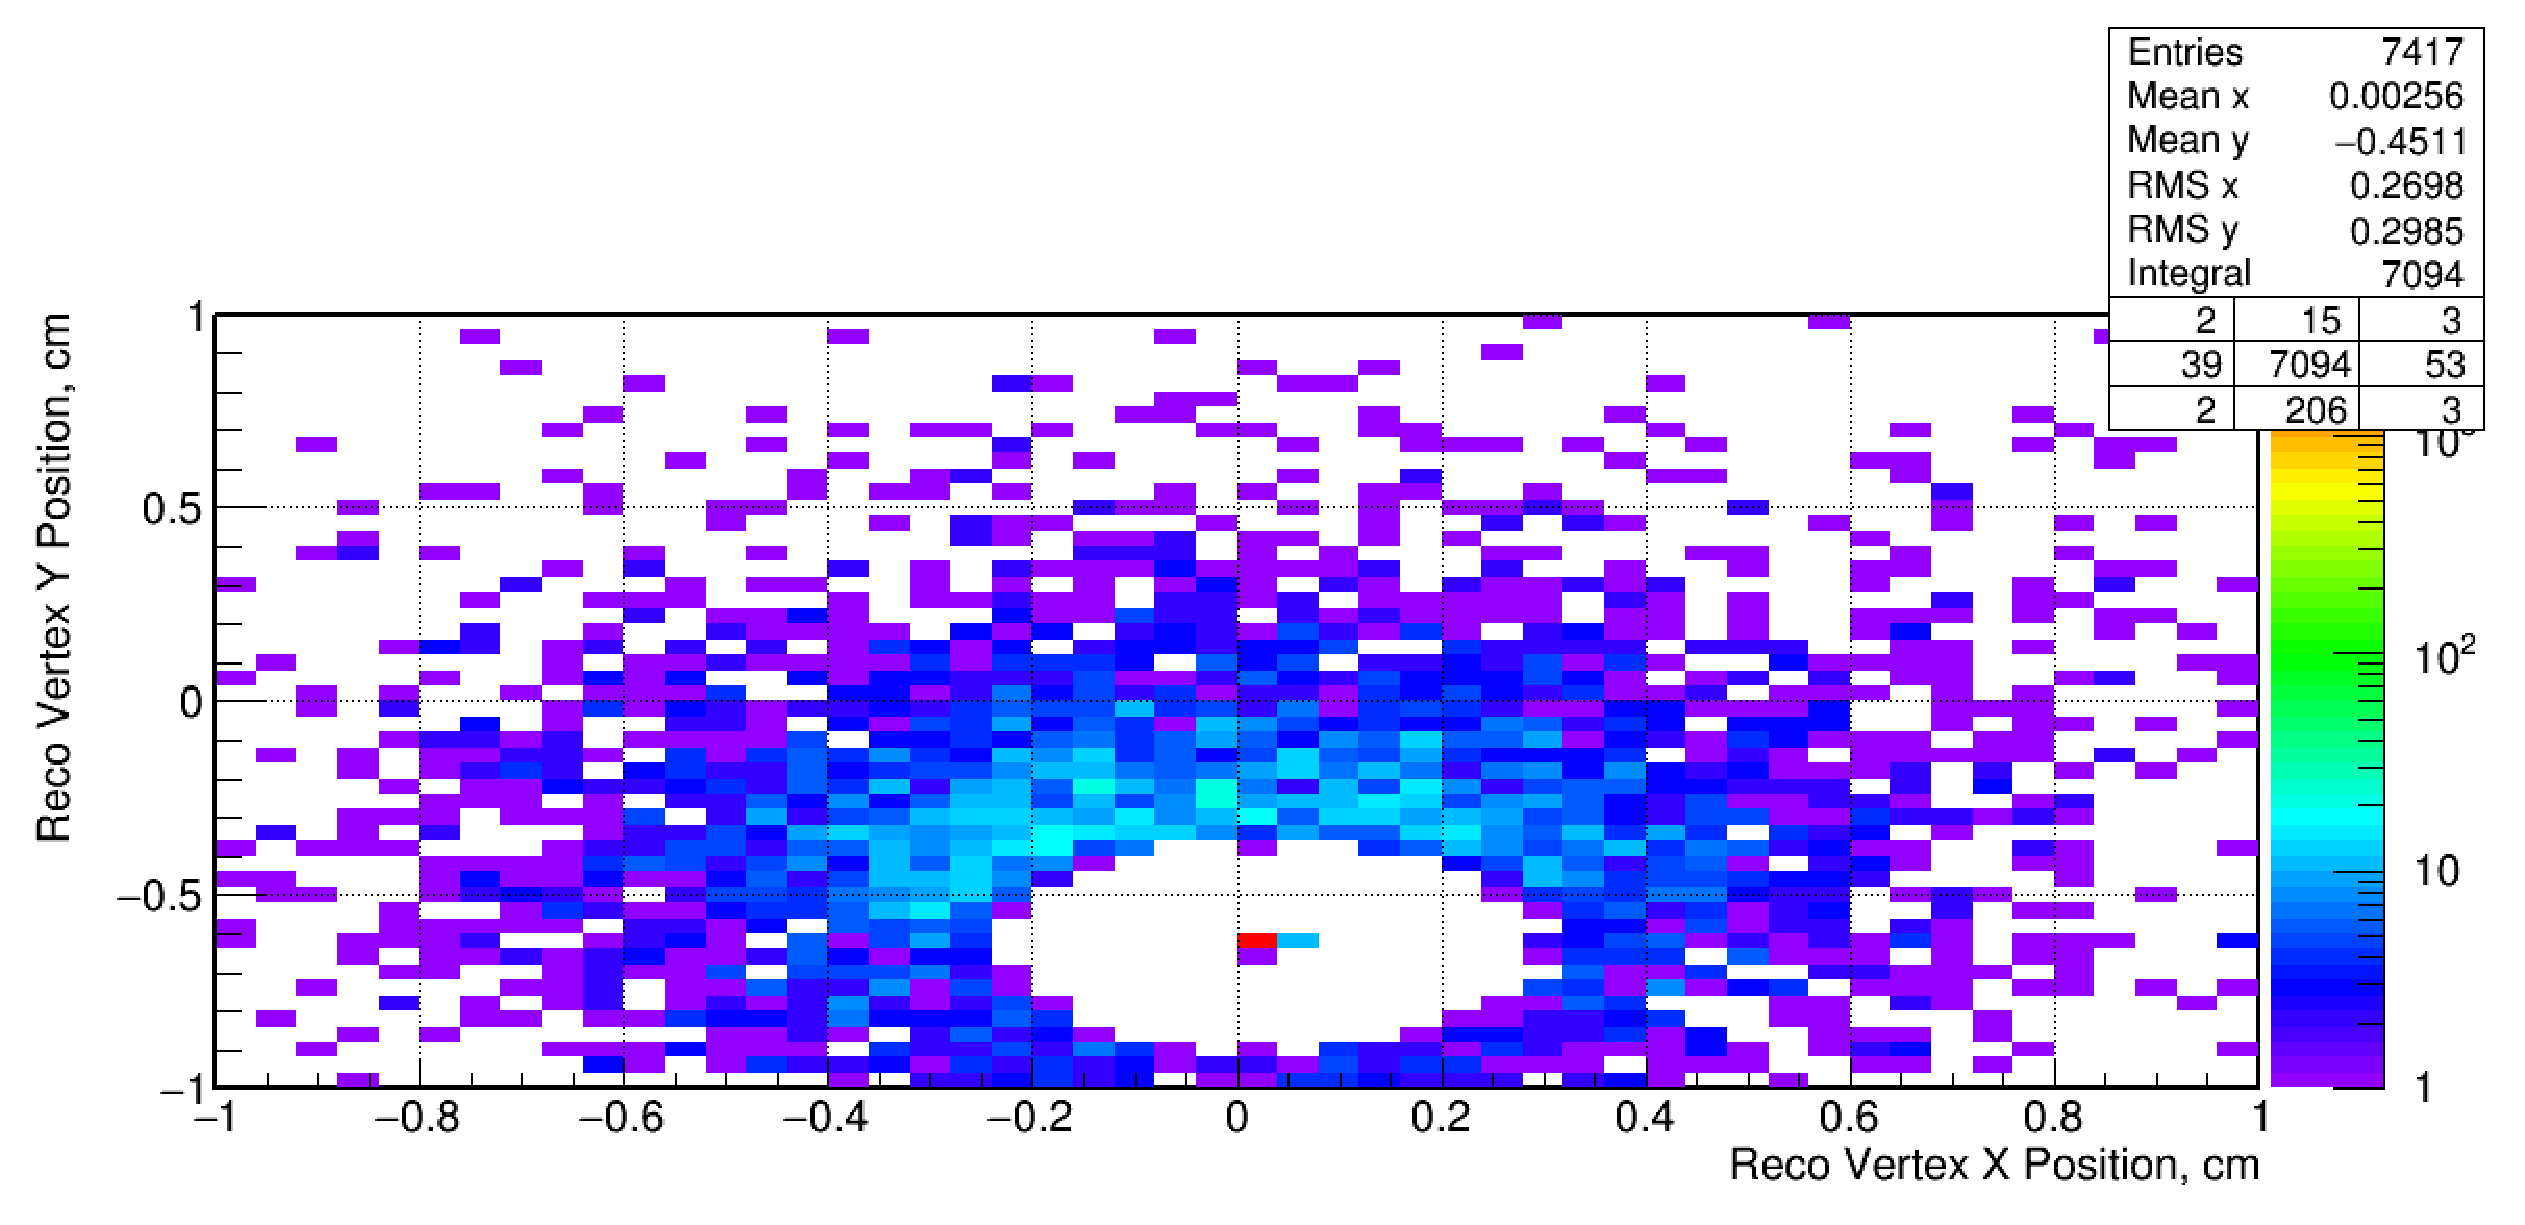
\includegraphics[height=0.25\textheight]{graphics/wemb_PPV_bl3D_s100_hVertexXvY} }
\rput[r](1\textwidth,0.10\textheight){ 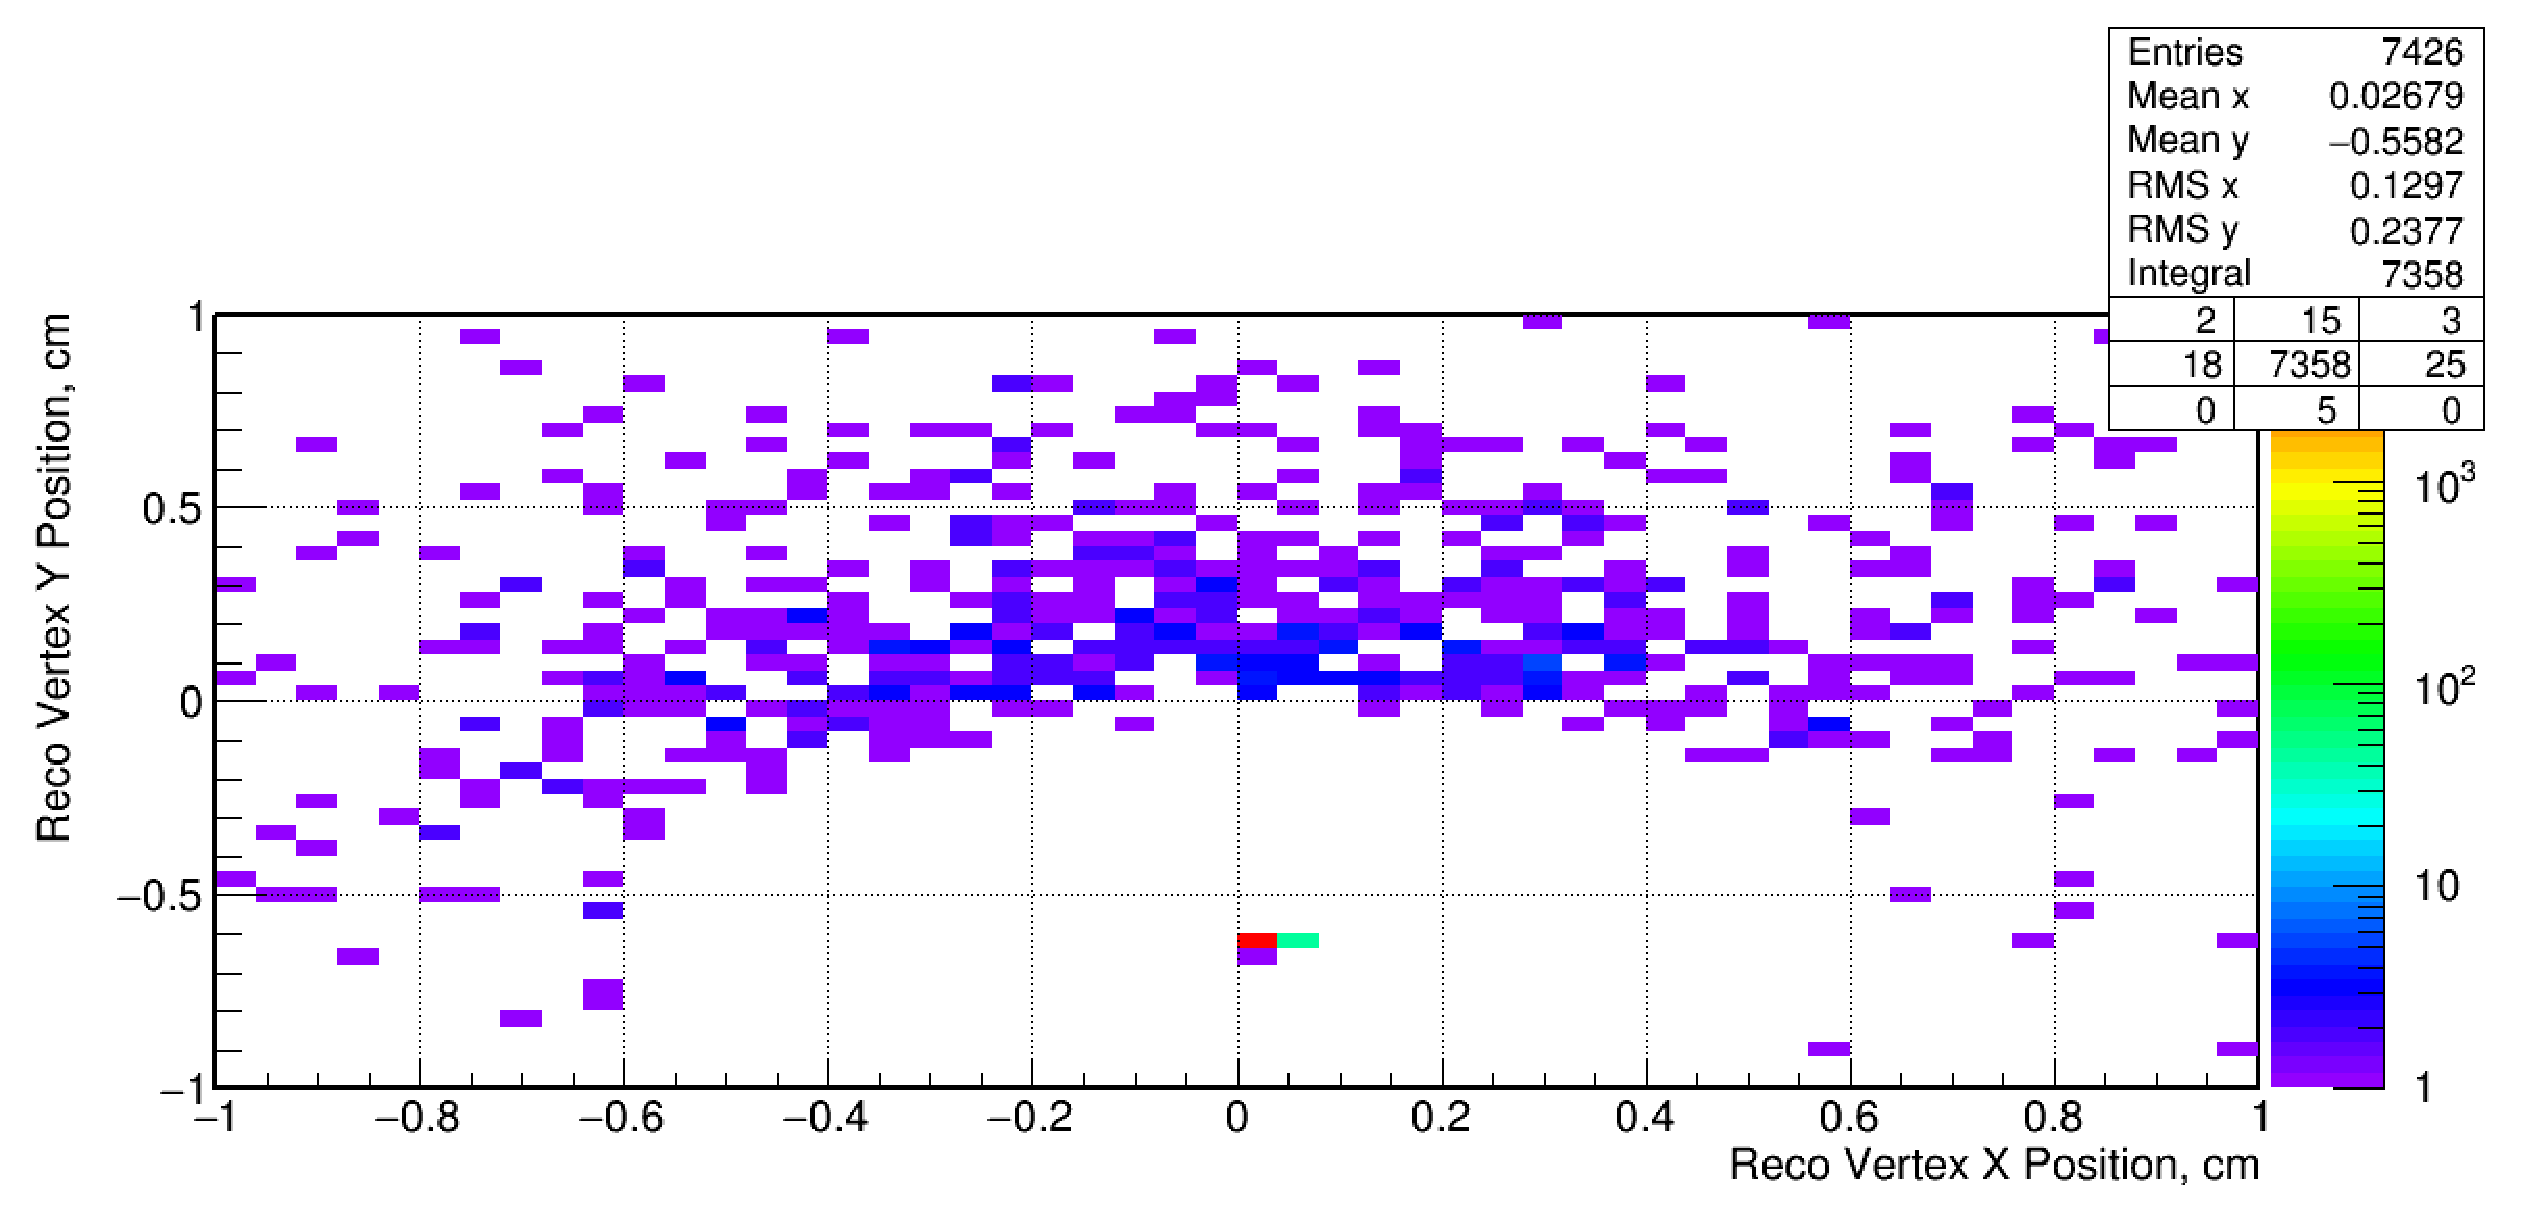
\includegraphics[height=0.25\textheight]{graphics/wemb_PPV_bl3D_s500_hVertexXvY} }


\rput[r](0.62\textwidth,0.45\textheight) {%
\begin{minipage}{0.60\textwidth}

\raggedright

\begin{list}{\labelitemi}{\setlength{\itemsep}{5mm}
                          \setlength{\topsep}{0mm}}

   \item In presence of HFT, high precision pile-up tracks can significantly
   bias primary vertex due to acceptance of such tracks at seeding phase

   \item This effect is alleviated by limiting contribution from measurements
   many sigmas away from the vertex candidate

   \item The usual $\chi^2$ function is modified as% defined as (``robust potential''):
   %
   \begin{equation*}
   f = \sum_{\text{tracks}} k_\text{seed} \left(1 - e^{ -\frac{\chi^2_\text{track}}{k_\text{seed}} } \right)
                          %+ k_\text{beam} \left(1 - e^{ -\frac{\chi^2_\text{beam} }{k_\text{beam}} } \right)
   \end{equation*}
   %
   where $k_\text{seed} > 0 $ is an adjustable scale factor% and $k_\text{beam} > 0 $ are adjustable scale factors


   \item \textbf{Similarly, vertex fits with high precision beamline contribution
   benefit from ``robust potential'' by avoiding track originated from
   secondarty vertices}

\end{list}

\end{minipage}
}


%\psgrid[gridlabels=0.7,subgriddiv=0, griddots=3](1,-1)(0,-3)(\textwidth,\textheight)

\end{pspicture}
%}}}



%===============================================================================
\myfoilhead{-30mm}{Using Beamline in Vertex Fit}
%{{{

\noindent
\begin{pspicture}(0,0)(\textwidth,\textheight)

\rput[lt](-2\unitlength,0.95\textheight){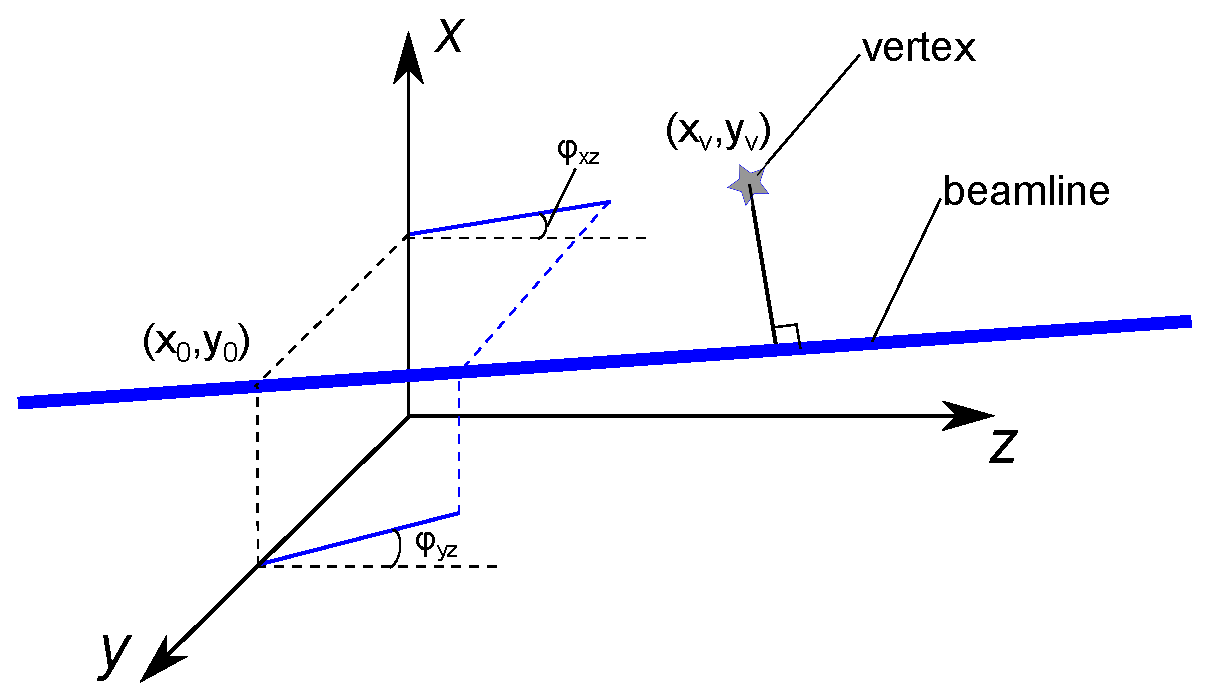
\includegraphics[width=0.6\textwidth]{graphics/beamline_3d}}


\rput[t](0.77\textwidth,0.93\textheight) {%
\begin{minipage}{0.45\textwidth}

\raggedright

\begin{list}{\labelitemi}{\setlength{\itemsep}{0mm}
                          \setlength{\topsep}{0mm}}

   \item Beamline parameters with uncertainties extracted from a global fit to tracks projected to $z$ axis

   \item Neglecting the correlation between the observables the beamline equation is trivial:
   %
   \begin{align*}
      x &= x_0 + k_{xz} z \quad &%
         \multirow{2}{0.5\linewidth}[2\unitlength]{%
            \raggedright with corresponding uncertainties for intercepts and slopes:\\ $\Delta{x_0}$, $\Delta{y_0}$,\\ $\Delta{k_{xz}}$, $\Delta{k_{yz}}$ } \\
      %
      y &= y_0 + k_{yz} z
   \end{align*}

\end{list}

\end{minipage}
}


\rput(0.5\textwidth,0.18\textheight) {%
\begin{minipage}{0.98\textwidth}

\raggedright

\begin{list}{\labelitemi}{\setlength{\itemsep}{0mm}
                          \setlength{\topsep}{0mm}}

   \item The full covariance matrix for DCA is also easily calculated:\\
   %
   \begin{equation*}
   \Sigma' = J \Sigma J^T\text{, with Jacobian for DCA w.r.t. the beamline parameters}
   \end{equation*}

   \item Beamline can be optionally applied to vertex fit as additional constraint
   %$f = \sum_{\text{tracks}} \chi^2_\text{track} + \chi^2_\text{beam}$

   \item The precision in transverse plane is only limited by intrinsic beam width and beam shape systematics ($\lesssim 100~\mu m$)

\end{list}

\end{minipage}
}


\rput[r](0.98\textwidth,-1\unitlength) {%
\footnotesize For implementation details see \url{https://github.com/star-bnl/star-vertex}
}


%\psgrid[gridlabels=0.7,subgriddiv=0, griddots=3](1,-1)(0,-3)(\textwidth,\textheight)

\end{pspicture}
%}}}



%===============================================================================
\myfoilhead{-30mm}{Secondary Decay Vertex}
%{{{

\noindent
\begin{pspicture}(0,0)(\textwidth,\textheight)

\rput[rb](0.48\textwidth,0.48\textheight){
\begin{pspicture}[showgrid=false](0.45\textwidth,0.45\textheight)%

\rput[lb](0,0){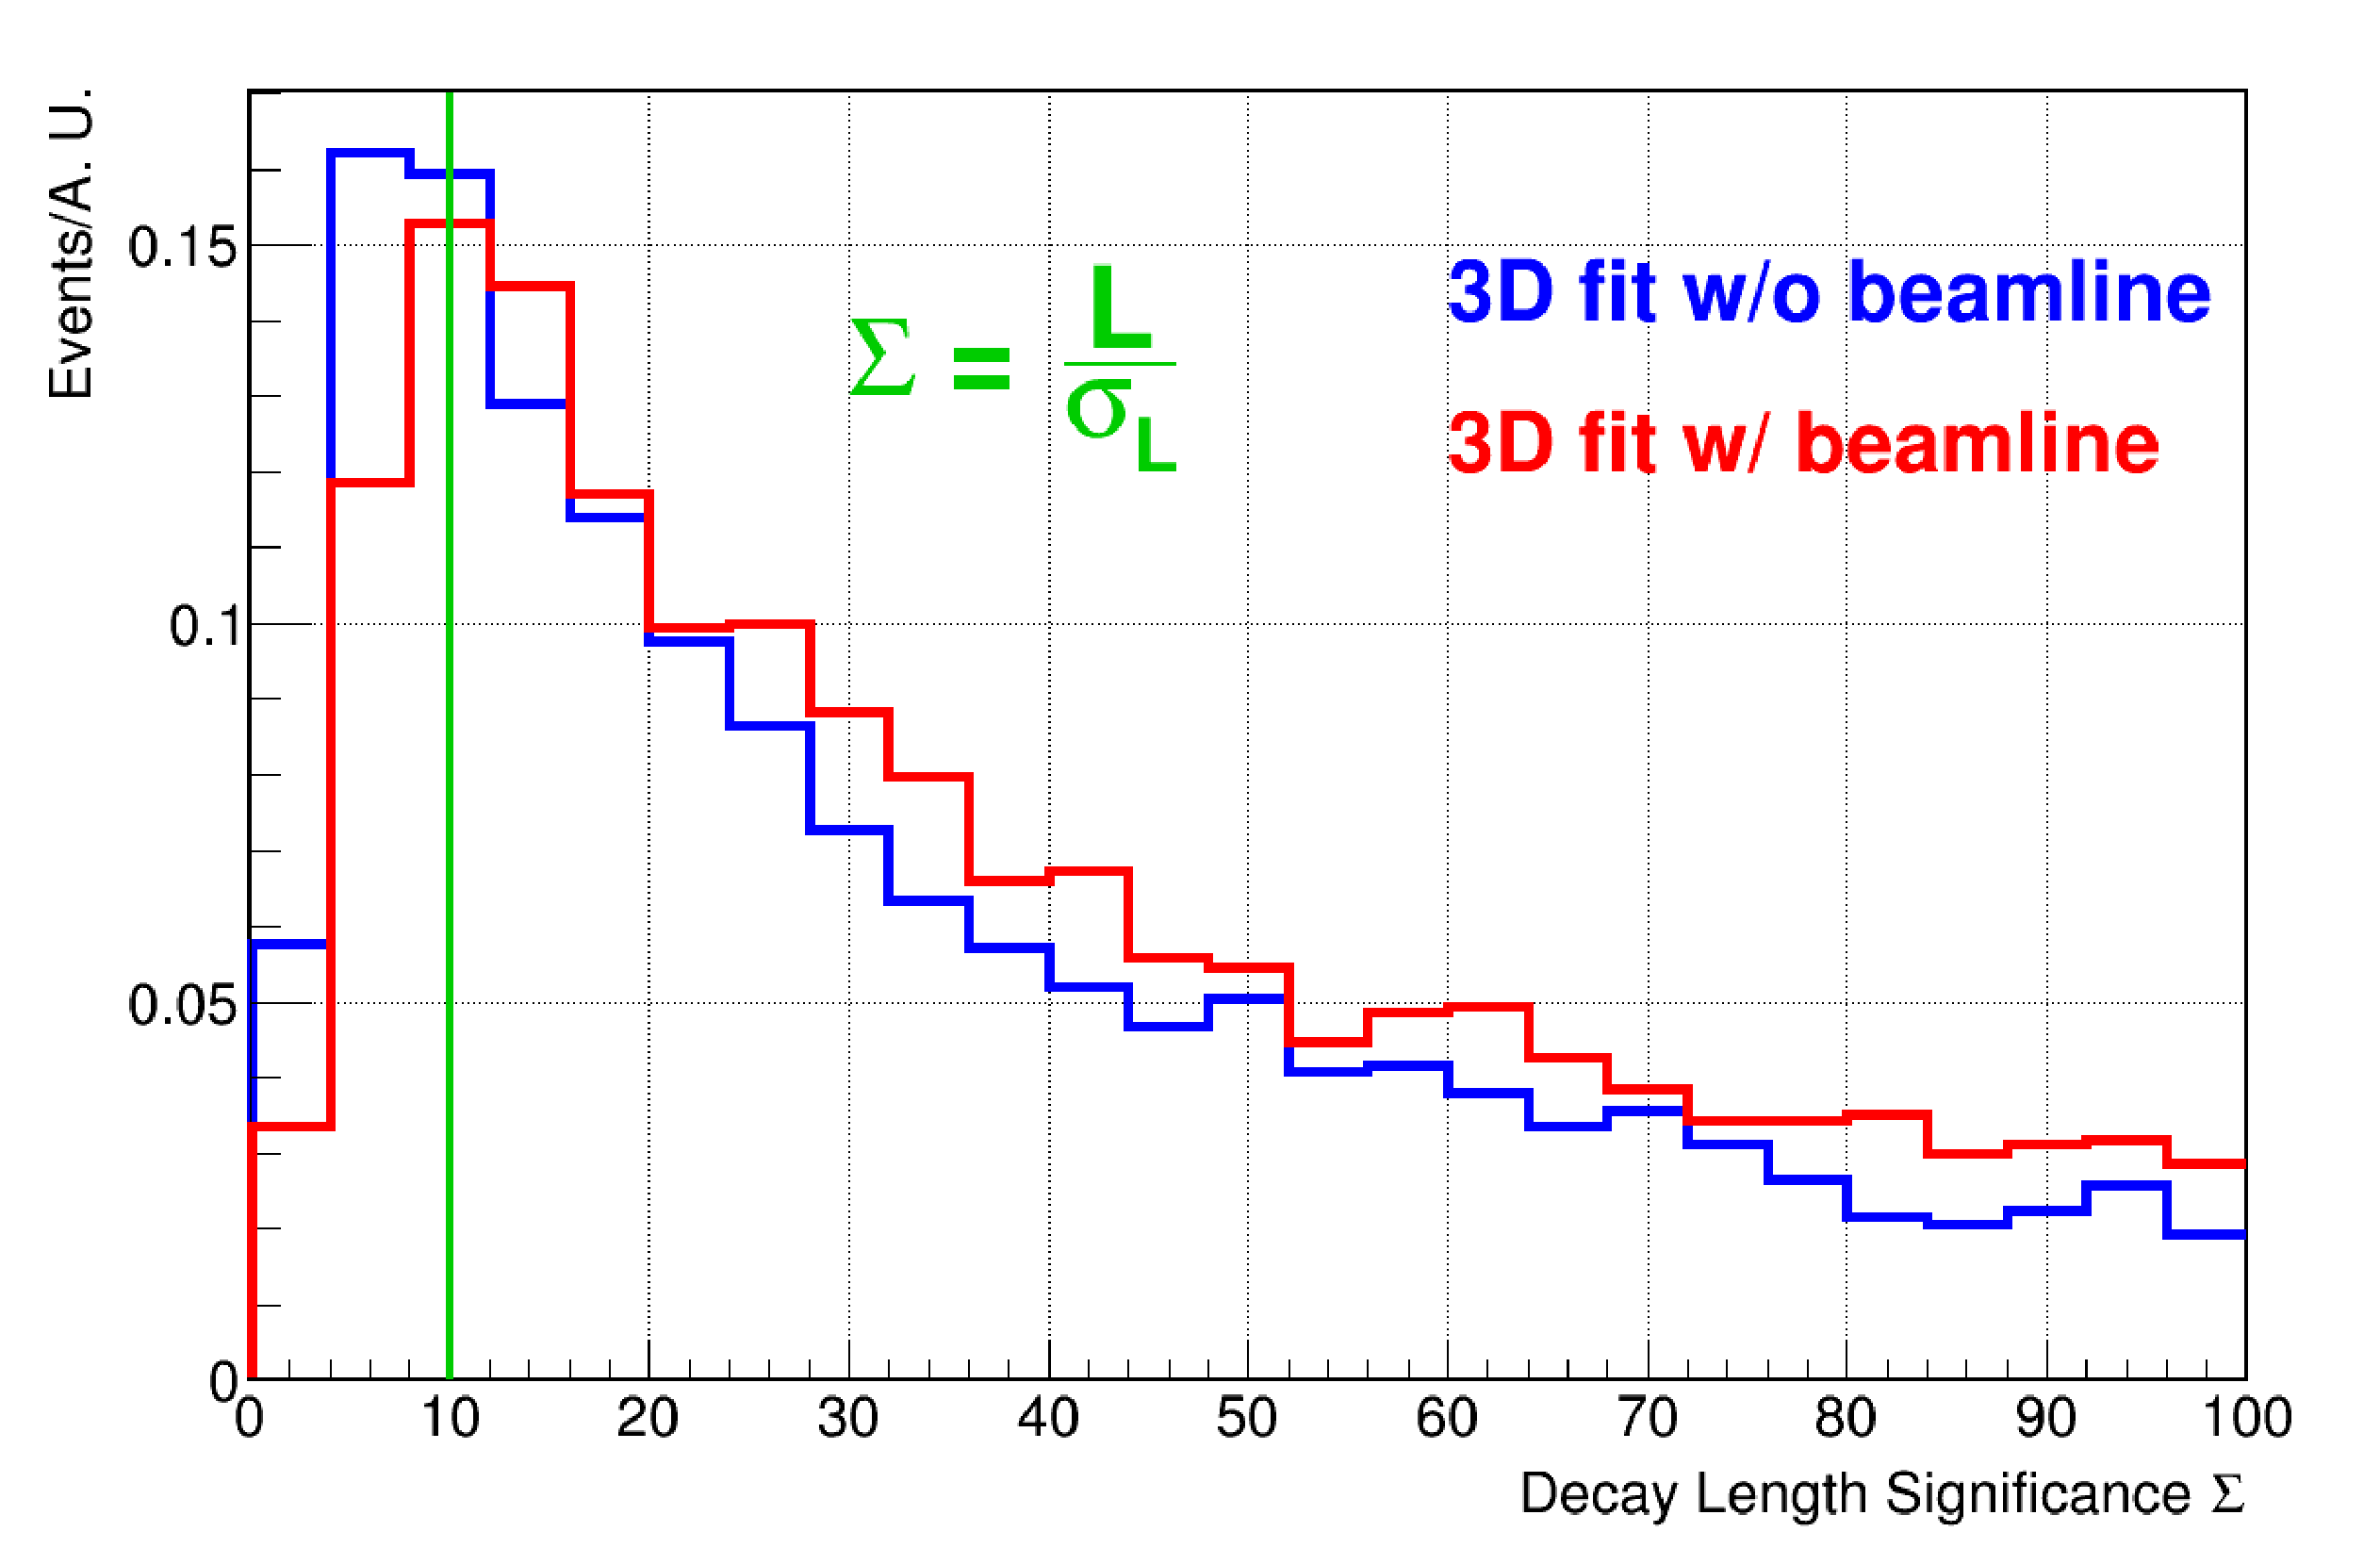
\includegraphics[width=0.45\textwidth]{graphics/lambda_decay_length_significance}}

% Labels
\rput[l](4.0, 3){ \footnotesize \textcolor{greenDark}{cut on secondaries} }
\rput(4.1, 3.7){ \pnode{from} }
\rput[l](9, 3.7){ \pnode{to} }
\ncline[linewidth=0.1, linecolor=greenDark, arrowscale=2]{->}{from}{to}

\end{pspicture} }

%\rput[rb](0.48\textwidth,0.48\textheight){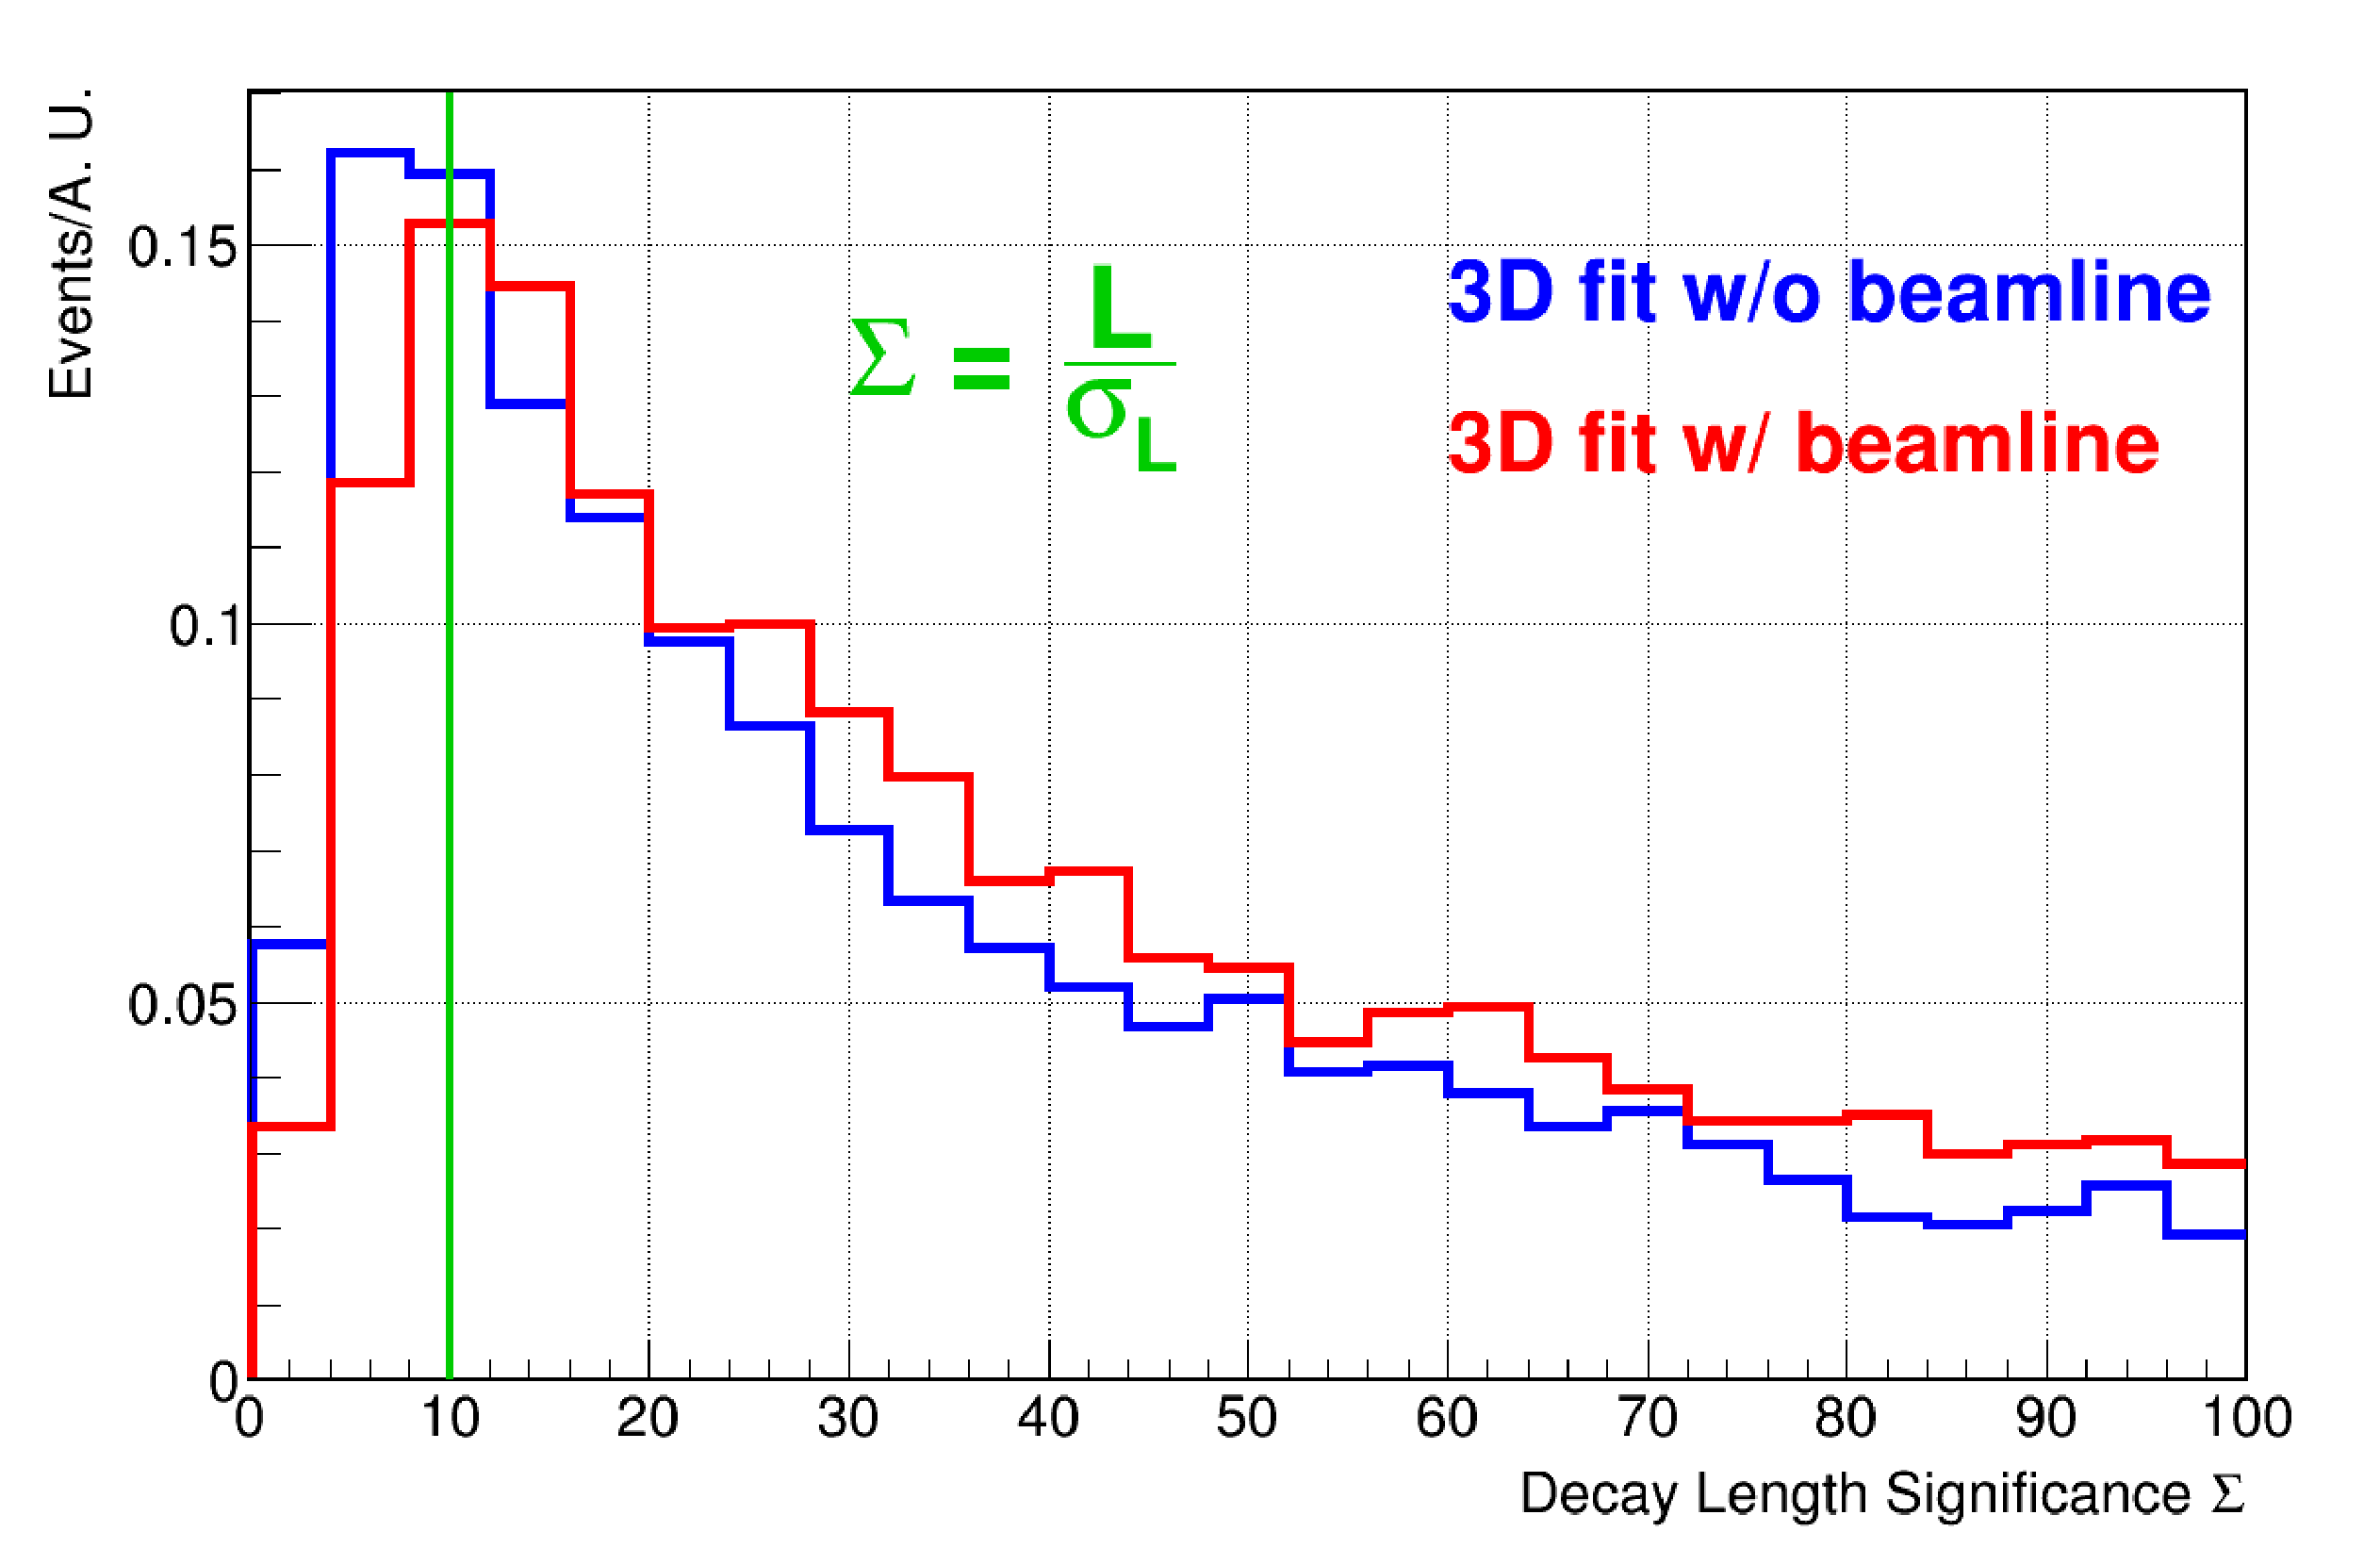
\includegraphics[width=0.45\textwidth]{graphics/lambda_decay_length_significance}}
\rput[lt](0.5\textwidth,0.45\textheight){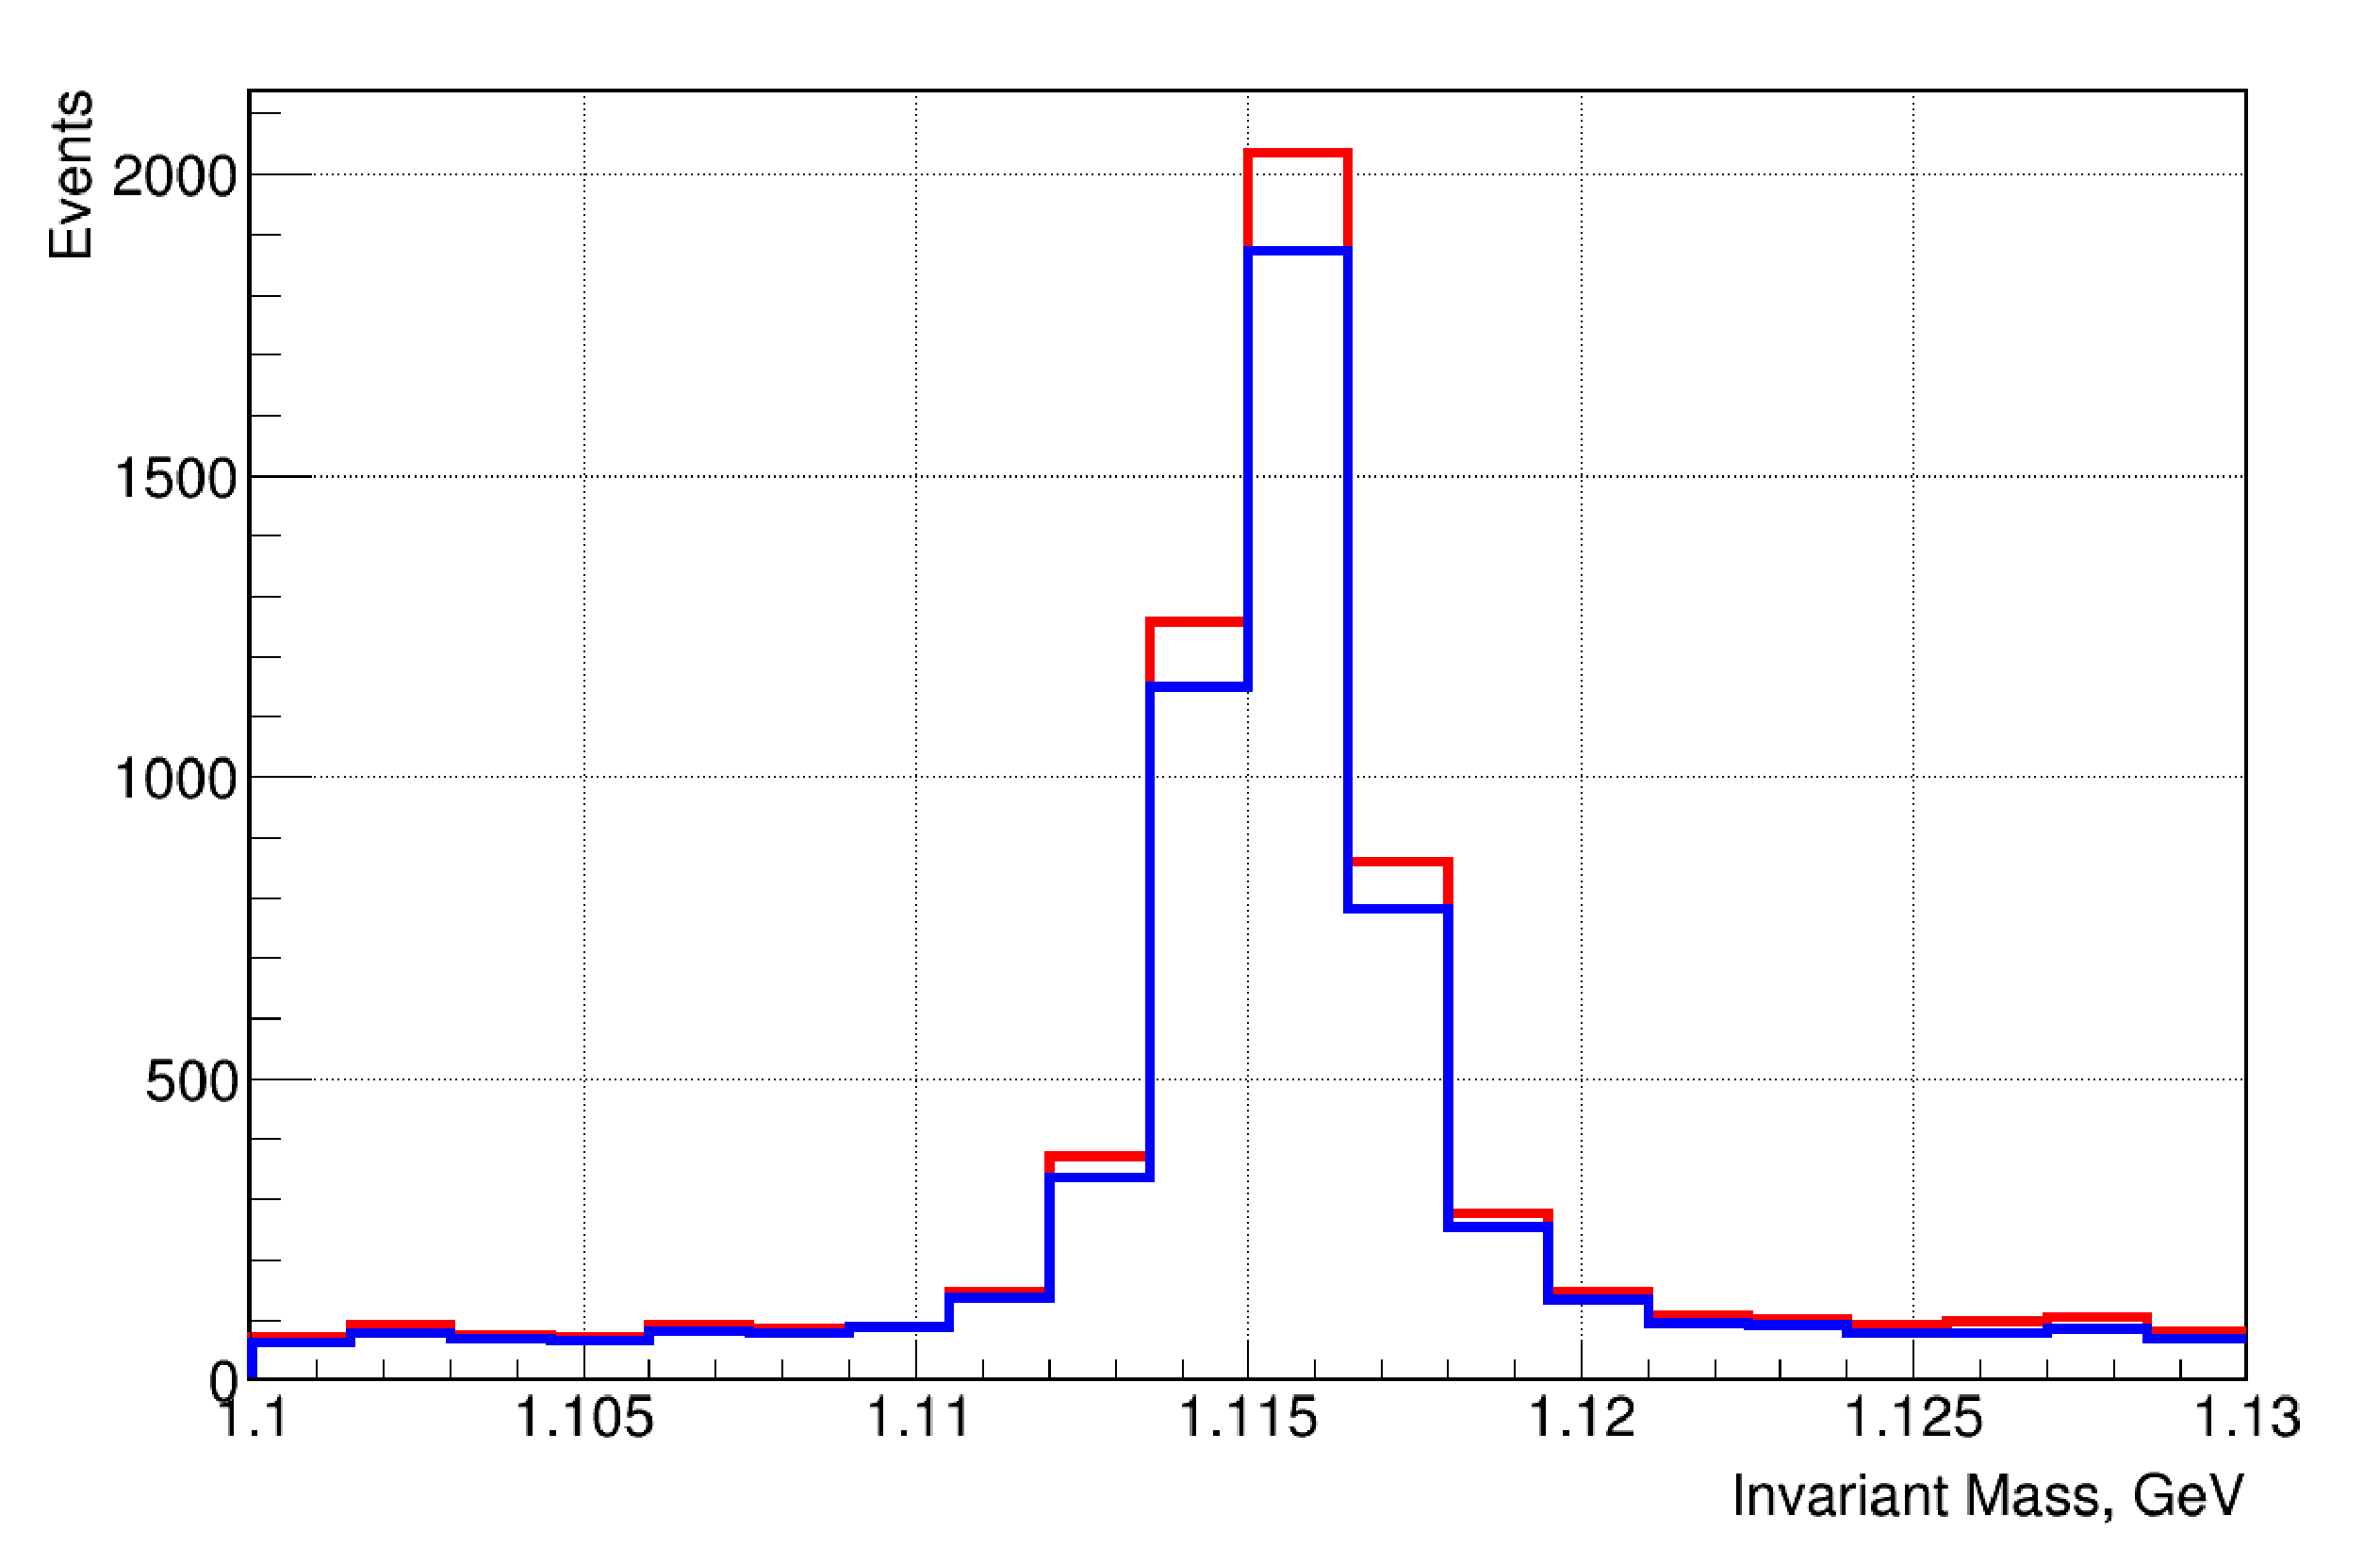
\includegraphics[width=0.45\textwidth]{graphics/lambda_inv_mass}}


\rput[l](29,11){ $\Lambda \to p \pi$ }


\rput[lb](0.48\textwidth,0.5\textheight) {%
\begin{minipage}{0.50\textwidth}

\raggedright

\begin{list}{\labelitemi}{\setlength{\itemsep}{0mm}
                          \setlength{\topsep}{0mm}}

   \item We test the effect of improved uncertainty on vertex position by
      reconstructing $\Lambda \to \pi p$ and $K^0 \to \pi p$ in simulated
      $pp$ collisions with pile-up

   \item We define decay length significance as $\Sigma = \frac{ \lvert \vec{v}_\text{prim} - \vec{v}_\text{decay} \rvert }{\sigma_v}$

   \item An indication of improvement in $S/B$ of $\approx 10\%$ is seen in reconstructed invariant mass of $\Lambda$ cadidates 

\end{list}

\end{minipage}
}


\rput[rt](0.5\textwidth,0.45\textheight) {%
\begin{minipage}{0.48\textwidth}

\raggedright

\begin{list}{\labelitemi}{\setlength{\itemsep}{0mm}
                          \setlength{\topsep}{0mm}}

   \item \textbf{New for STAR:} \\[2mm]

      \textcolor{blue}{\bf 3D fit w/o beamline}: Only tracks used in the 3D fit (both VFs) \\[2mm]
      \textcolor{red}{\bf 3D fit w/ beamline}: Beamline and tracks used in 3D fit

   \item \textbf{Previously:} \textcolor{black}{\bf 1D fit w/ beamline} \\[2mm]

      Primary vertex is forced to be on the beamline\\
      $\mathbf{\Rightarrow}$ no transverse uncertainties on primary vertex position

\end{list}

\end{minipage}
}


%\psgrid[gridlabels=0.7,subgriddiv=0, griddots=3](1,-1)(0,-3)(\textwidth,\textheight)

\end{pspicture}
%}}}



%===============================================================================
\myfoilhead{-30mm}{Common Tool for Performace Evaluation}
%{{{

\noindent
\begin{pspicture}(0,0)(\textwidth,\textheight)


\rput(0.50\textwidth,0.46\textheight) {%
\begin{minipage}{0.90\textwidth}

\raggedright

\textbf{\texttt{\large Travex:} \normalsize A toolkit for track and vertex reconstruction evaluation}\\[12mm]

\begin{list}{\labelitemi}{\setlength{\itemsep}{0mm}
                          \setlength{\topsep}{0mm}}

   \item \textbf{Standalone.} No dependencies on specific event data format

   \item \textbf{Experiment independent.} Focus on common physical observables

   \begin{list}{\labelitemii}{\setlength{\itemsep}{2mm}
                               \setlength{\topsep}{3mm}}
      
      \item Pull distributions, vertex position, resolution, etc.

      \item Vertex finding efficiency, (im)purity based on dominant contributor matches in simulation

   \end{list}

   %\item Designed with a typical workflow in mind:\\[2mm]
   %$\Rightarrow$ Interface user's event/track/vertex data structs with \texttt{Travex}\\[2mm]% to generic structures in \texttt{Travex}\\
   %$\Rightarrow$ Optionally create TTree\\[2mm]
   %$\Rightarrow$ Fill histograms and compare\\[12mm]

	\begin{center}
	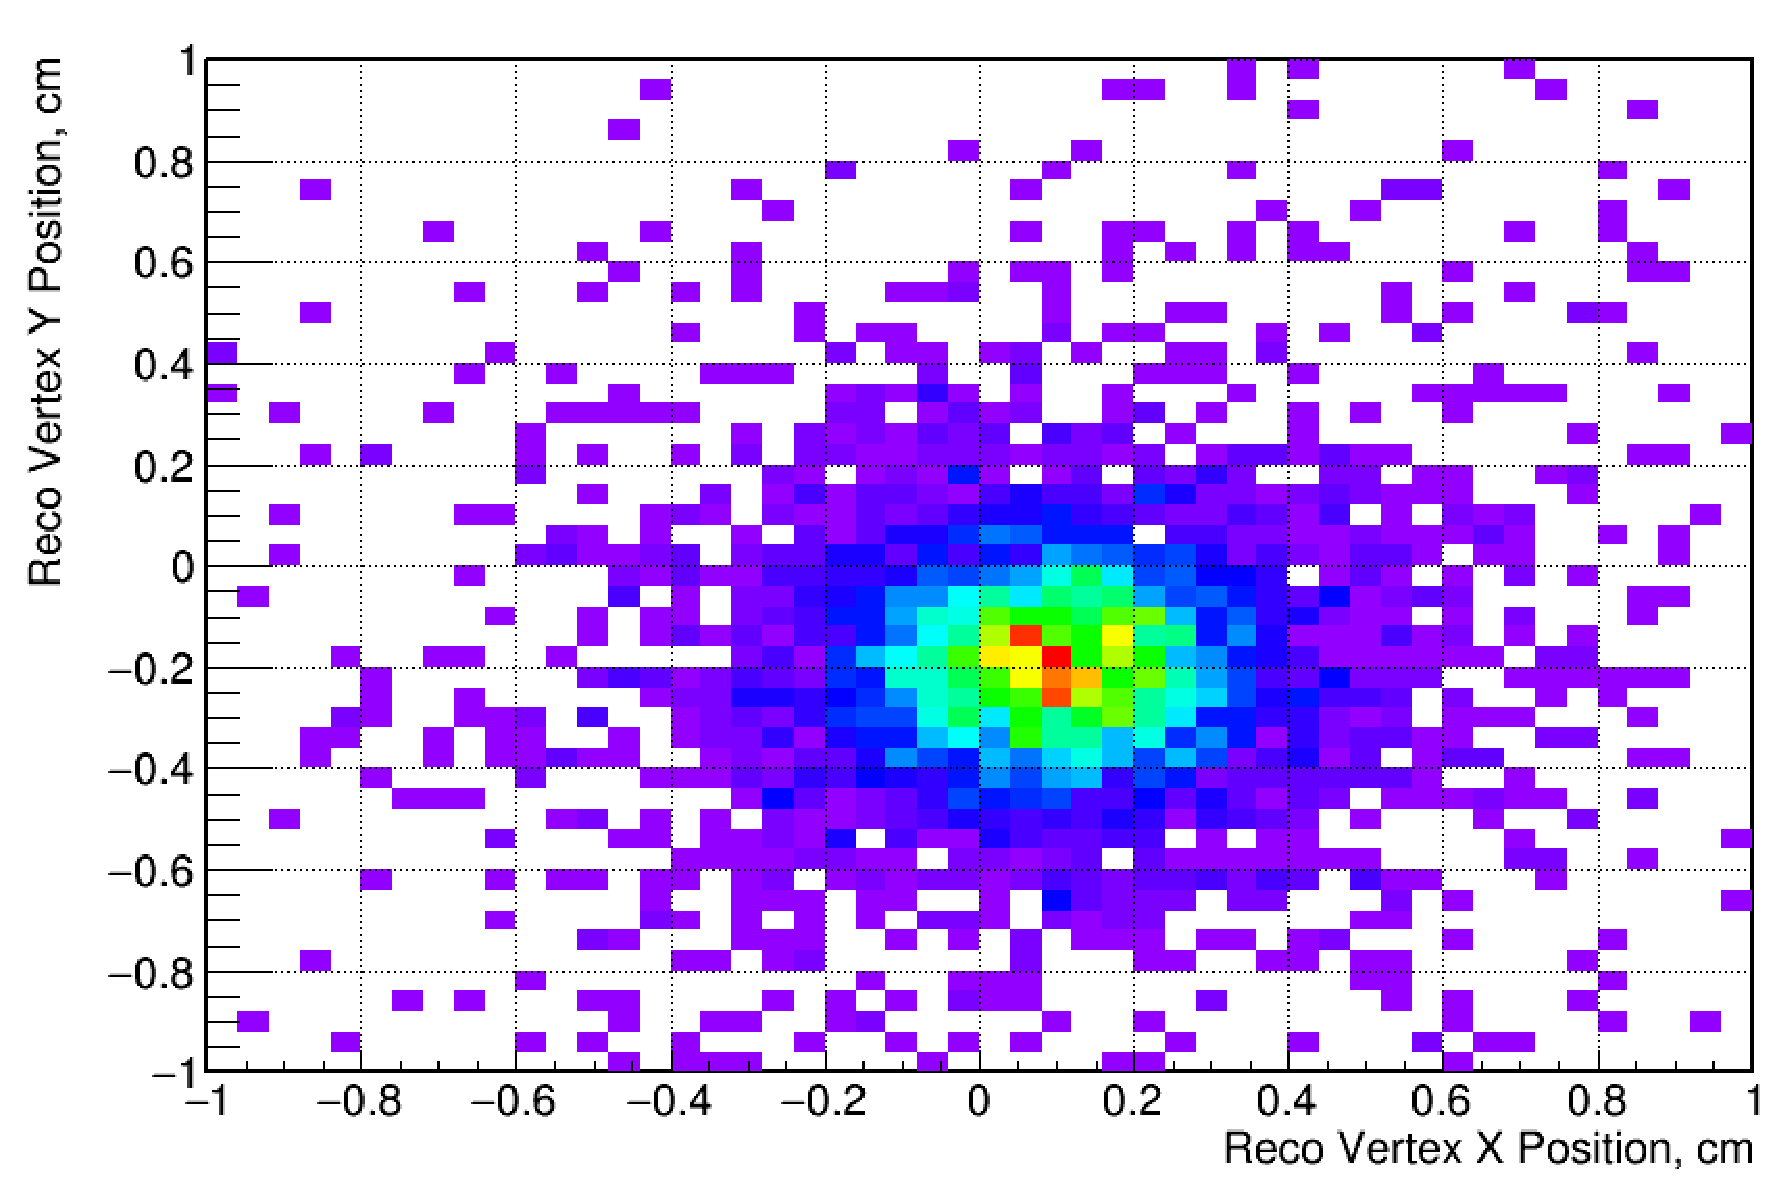
\includegraphics[height=0.25\textheight]{graphics/vtx_xy_minuitvf}
	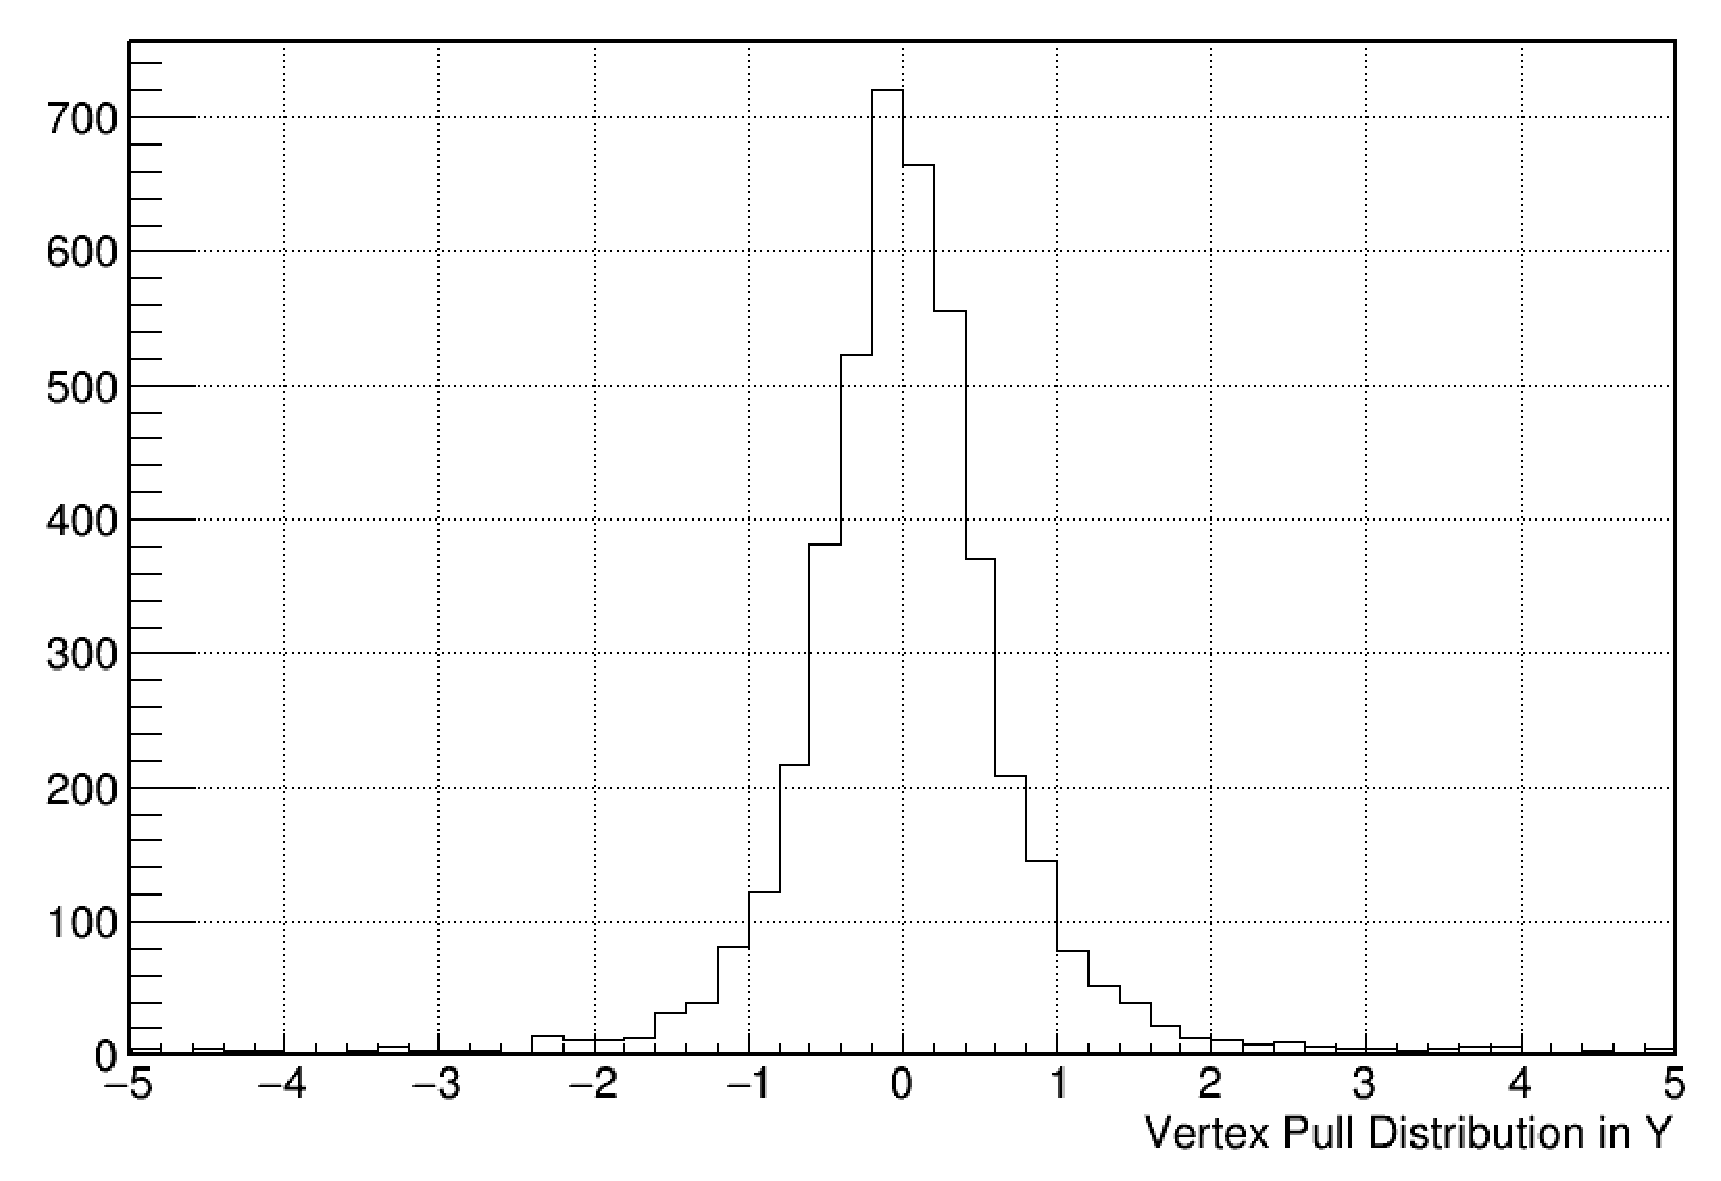
\includegraphics[height=0.25\textheight]{graphics/vtx_pull_y_minuitvf}
	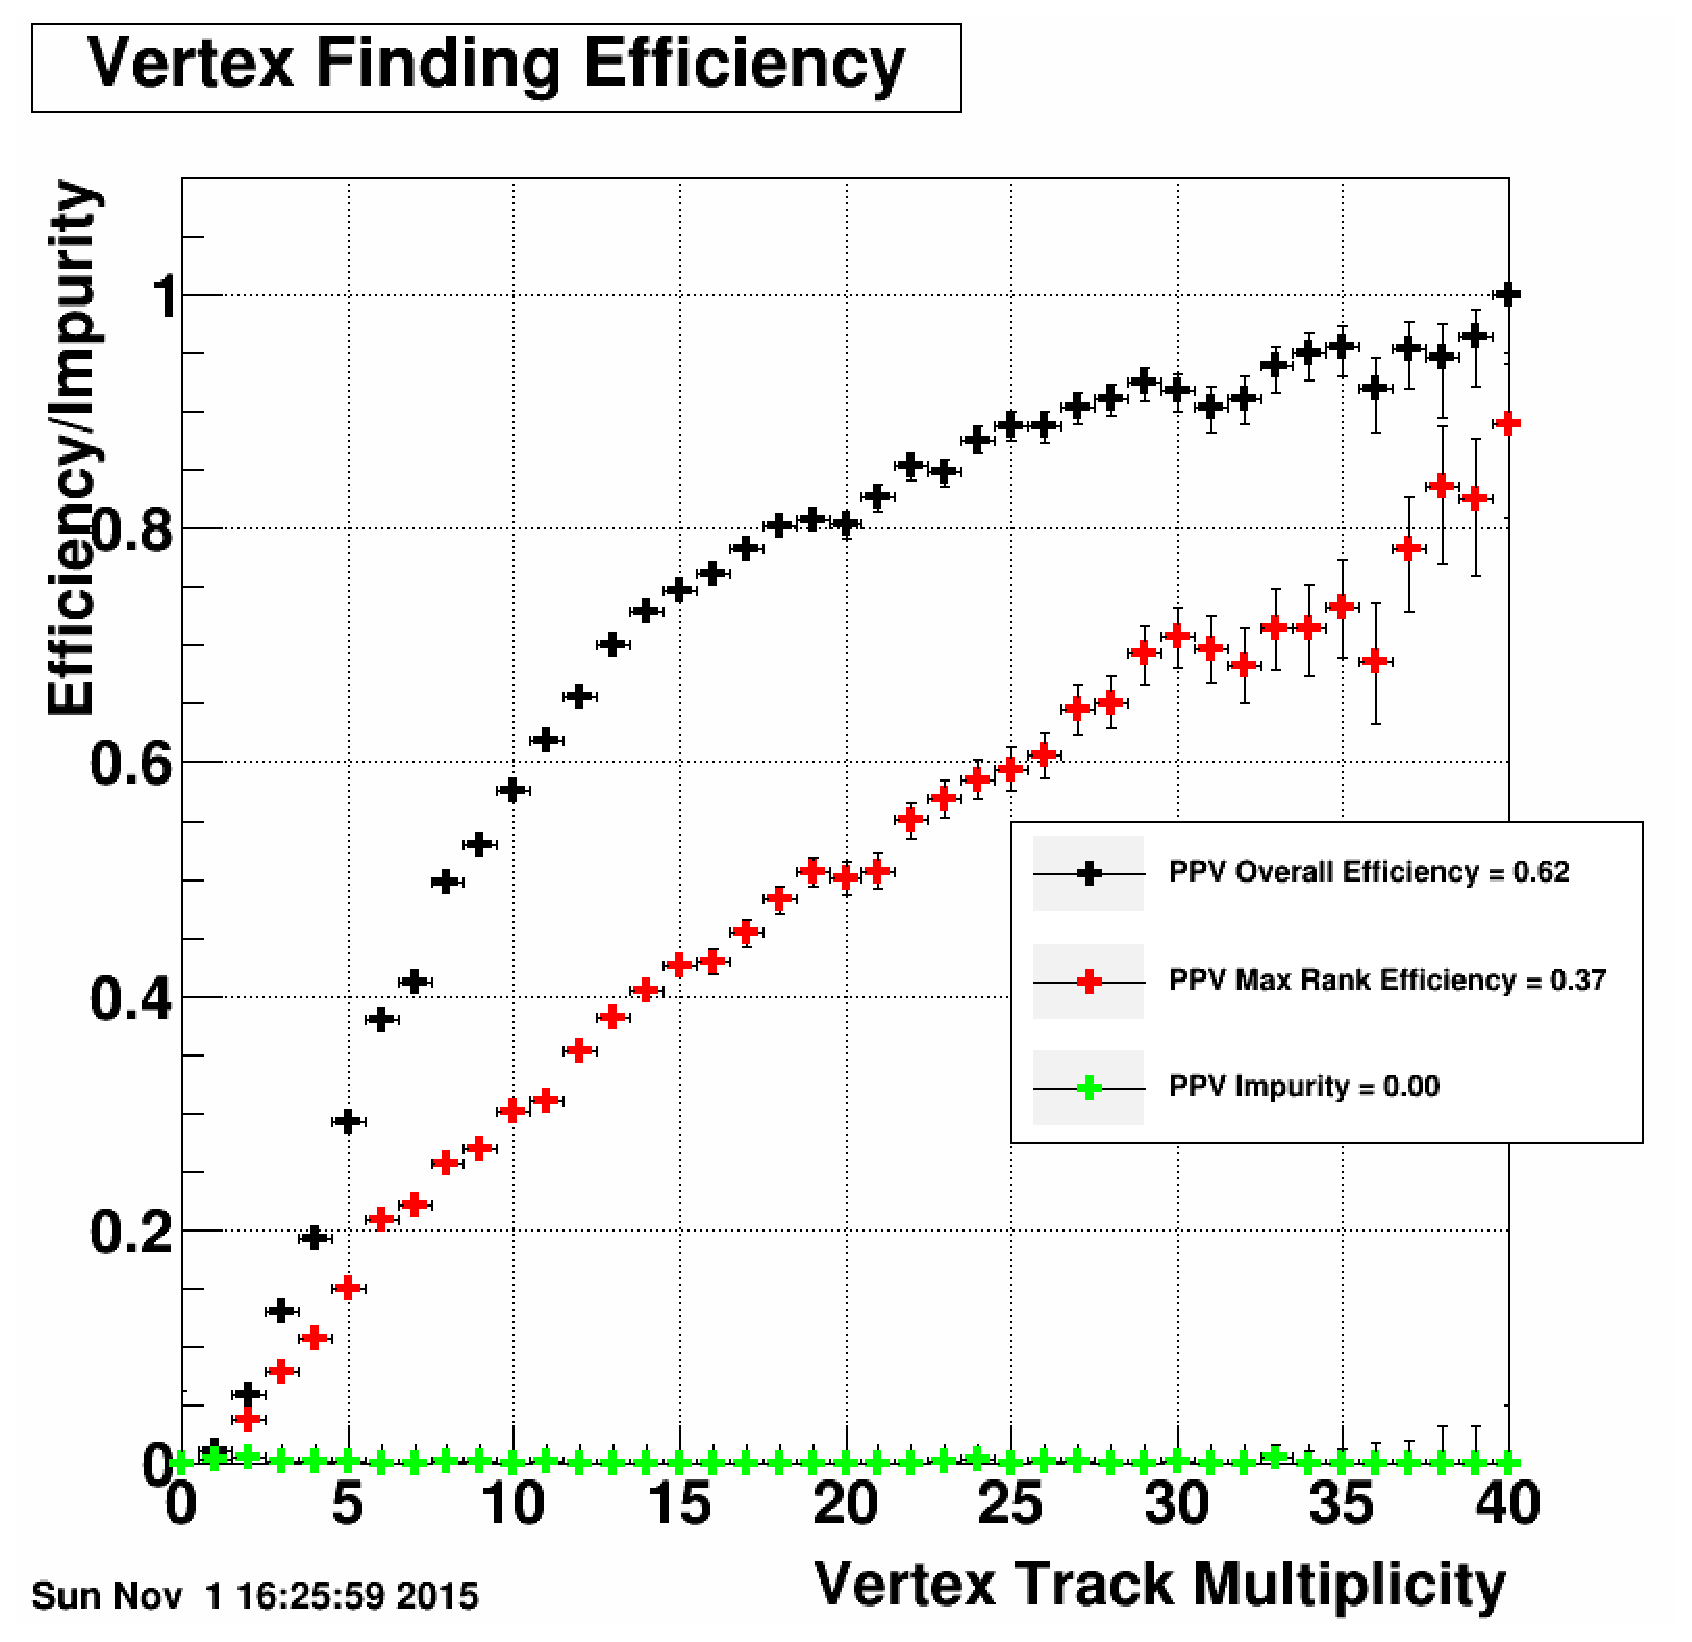
\includegraphics[height=0.25\textheight]{graphics/vtx_eff_ppv}
	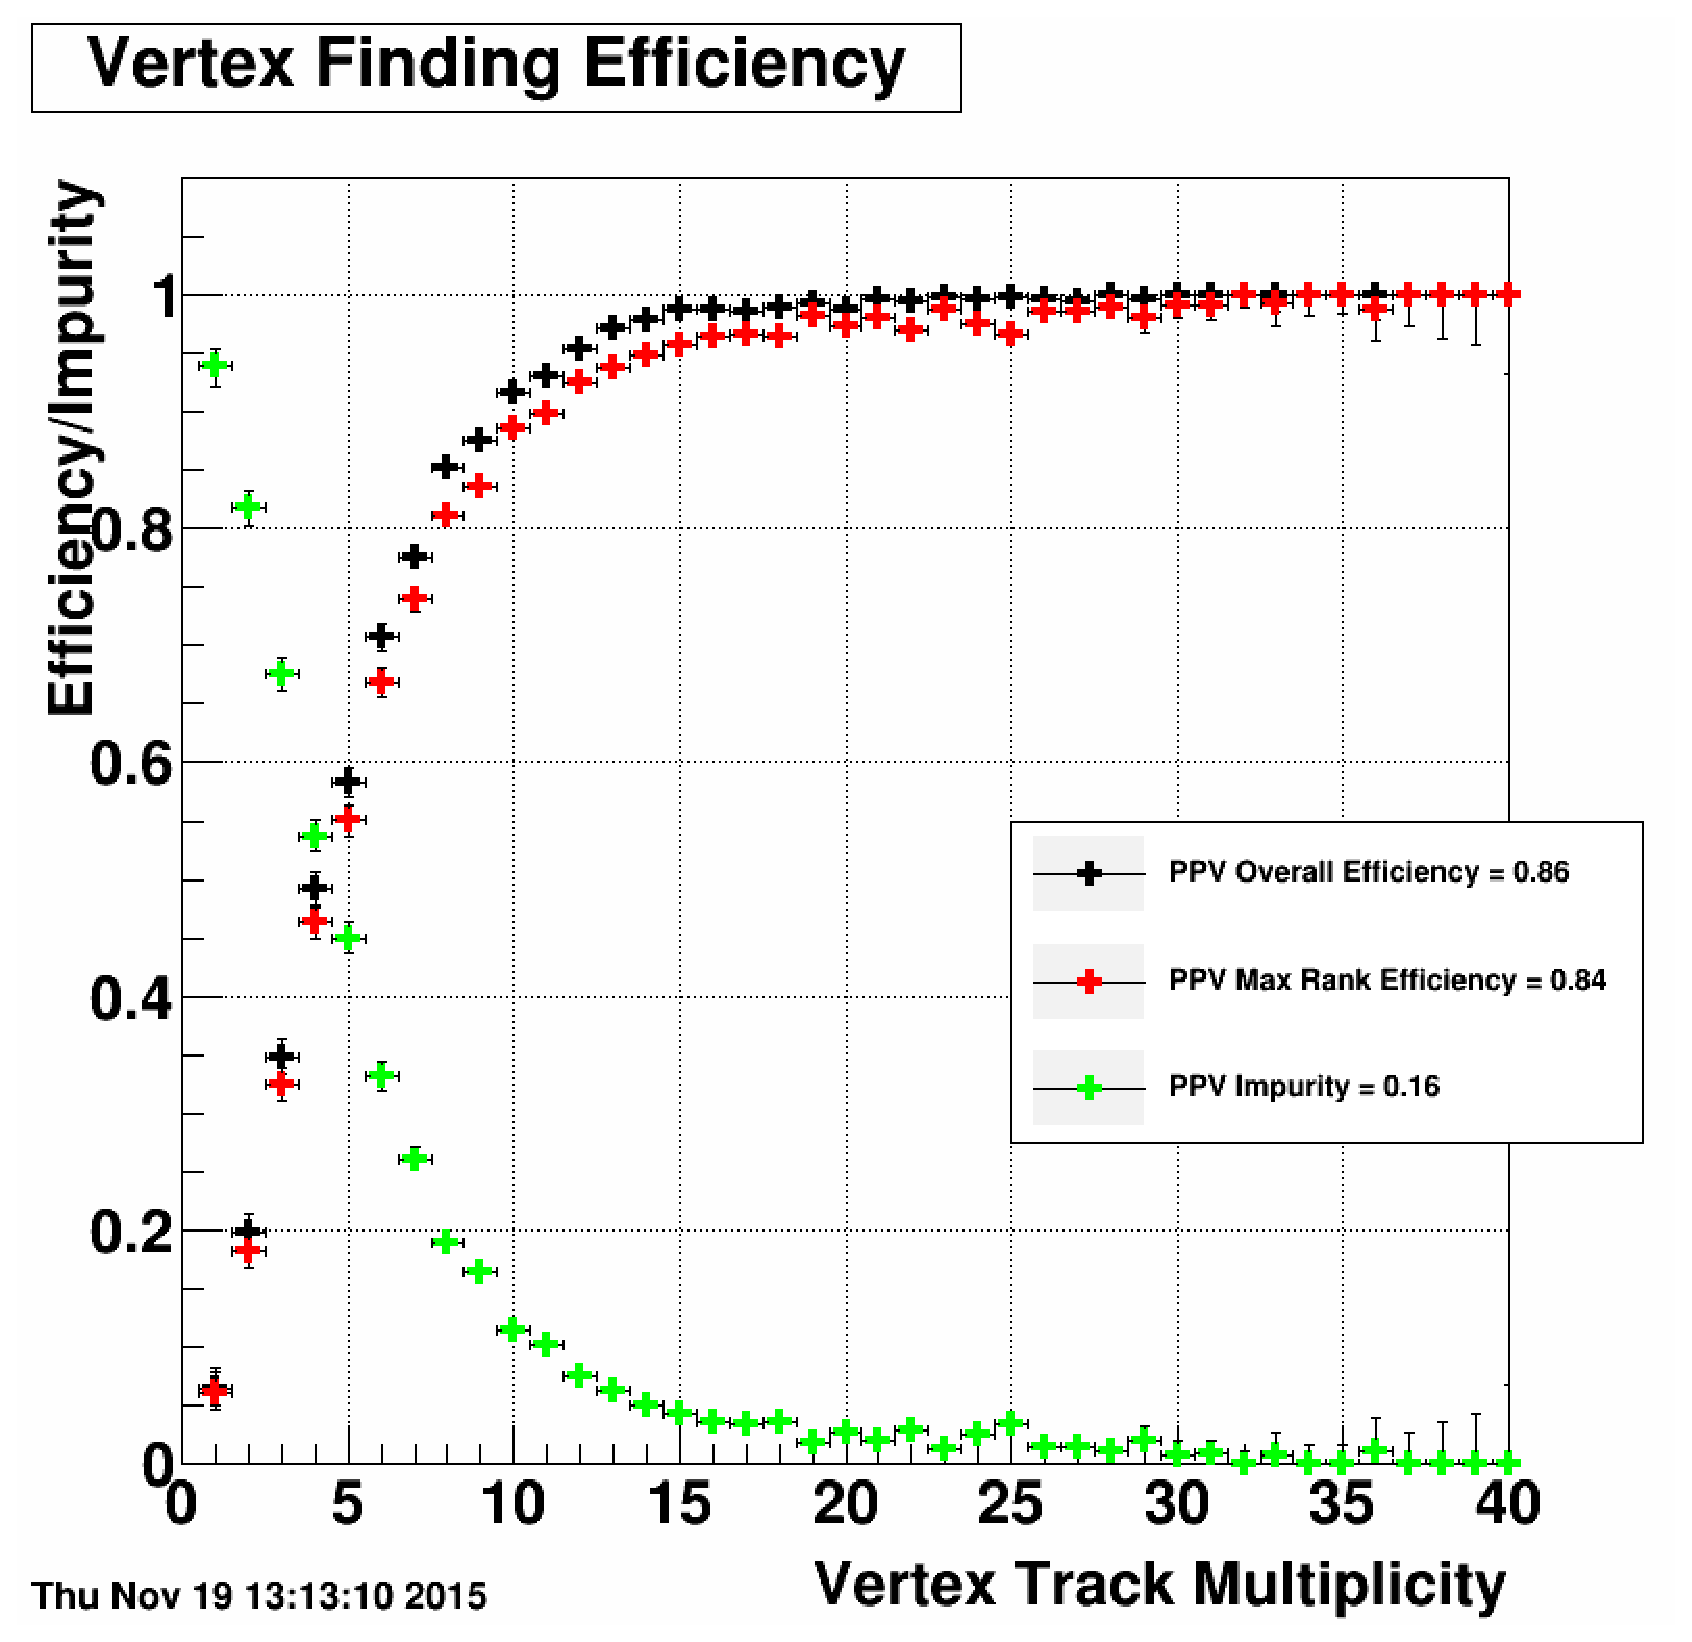
\includegraphics[height=0.25\textheight]{graphics/vtx_eff_ppv_extra_vtcs}
	\end{center}

	\hspace{10mm}

   \begin{center}
   \textbf{Source code openly available} \url{https://github.com/plexoos/travex}
   \end{center}

\end{list}

\end{minipage}
}


%\psgrid[gridlabels=0.7,subgriddiv=0, griddots=3](1,-1)(0,-3)(\textwidth,\textheight)

\end{pspicture}
%}}}



%===============================================================================
\myfoilhead{-30mm}{Summary}
%{{{

\noindent
\begin{pspicture}(0,0)(\textwidth,\textheight)


\rput[lt](0.06\textwidth,0.85\textheight) {%
\begin{minipage}{0.90\textwidth}

\raggedright

\begin{list}{\labelitemi}{\setlength{\itemsep}{0mm}
                          \setlength{\topsep}{0mm}}

   \item STAR employs several techniques to overcome pile-up contamination in vertex reconstruction in TPC
      
   \begin{list}{\labelitemii}{\setlength{\itemsep}{0mm}
                              \setlength{\topsep}{0mm}}

      \item Vertex ranking based on fast non-tracking detectors
      \item Rejection of split tracks

   \end{list}

   \item Developed tools and algorithms can be used by other experiments

   \begin{list}{\labelitemii}{\setlength{\itemsep}{0mm}
                              \setlength{\topsep}{0mm}}

      \item Laid the groundwork for seamless comparison of vertex finders $\Rightarrow$
		\href{https://github.com/plexoos/travex}{\texttt{code}}

   \end{list}

\end{list}

\end{minipage}
}


\rput[l](0.68\textwidth,0.22\textheight){ 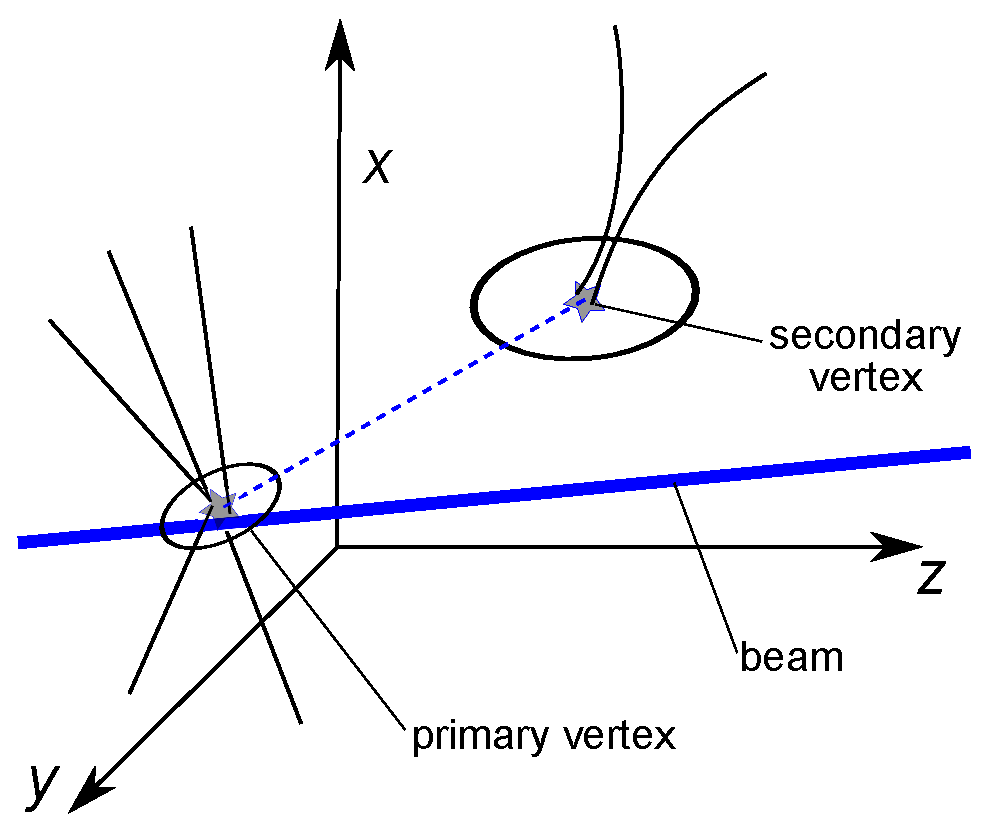
\includegraphics[width=0.28\textwidth]{graphics/beamline_primary_secondary_3d} }

\rput[l](0.06\textwidth,0.22\textheight) {%
\begin{minipage}{0.62\textwidth}

\raggedright

\begin{list}{\labelitemi}{\setlength{\itemsep}{0mm}
                          \setlength{\topsep}{0mm}}

	\item \textbf{STAR vertex finders have been enhancement by implementing 3D
	fits to primary vertices with proper beamline constraint and reporting of
	real uncertainties}

   \begin{list}{\labelitemii}{\setlength{\itemsep}{3mm}
                              \setlength{\topsep}{0mm}}

      \item Certain analyses relying on topology cuts may benefit from using the new vertex uncertainties
			%our initial study has indicate potential improvement 

	   \item In $\Lambda$-enriched sample with realistic pile-up we observed an improvement in $S/B$ of $\sim 10\%$

   \end{list}

\end{list}

\end{minipage}
}


%\psgrid[gridlabels=0.7,subgriddiv=0, griddots=3](1,-1)(0,-3)(\textwidth,\textheight)

\end{pspicture}
%}}}



%===============================================================================
\label{slide:last}

\end{document}
